
The results present two predictors, ExoType and ExoTarget, that can differentiate between bacterial exotoxin types and targets based different inputs such as protein sequences and protein folds.
This section introduces the data processing, steps of machine learning pipeline and model evaluation based on metrics.

\subsection{Data Exploration and Preprocessing}
In this section, the data distribution among types and targets is explained. Then, it discusses how the raw data is preprocessed through redundancy reduction techniques.

\subsubsection{Dataset Overview}
\begin{figure}[H]
	\centering
	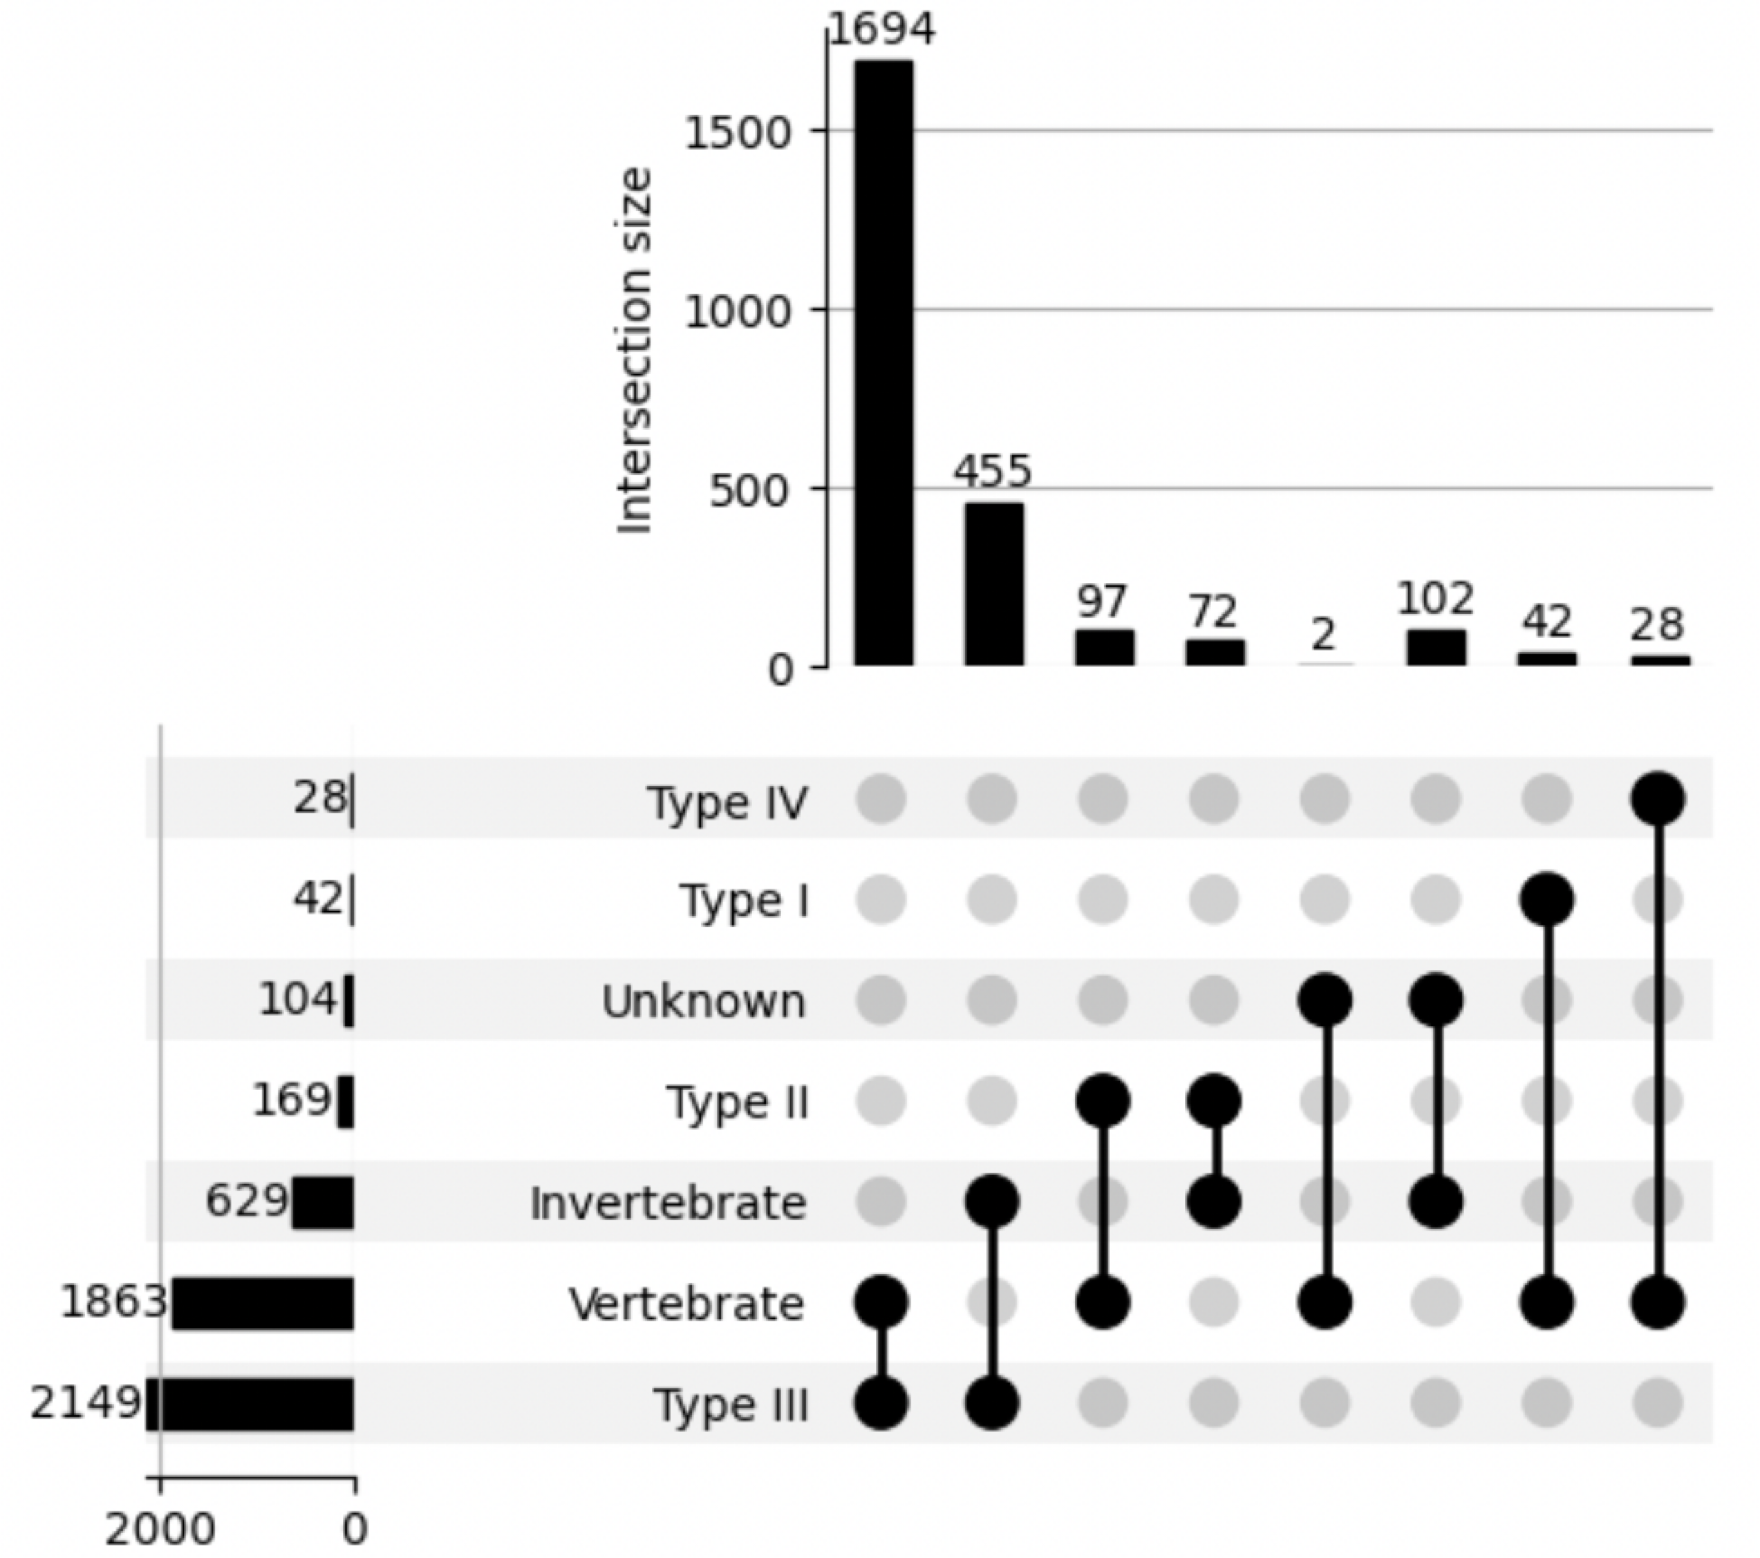
\includegraphics[width=0.8\textwidth]{images/upset_plot_of_raw_data.png}
	\caption{Upset plot illustrating the distribution of exotoxin types and their host targets. 
		The plot consists of two main sections: a bar chart at the top and a matrix plot below. 
		The bar chart, located in the upper part of the figure, represents the intersection size of different categories in black bars. The tallest bar, reaching approximately 1,694, corresponds to the most frequent category intersection. The lower part of the figure presents a matrix of black-filled circles and gray background dots. Each row corresponds to a bacterial exotoxin type or host target category, including Type I, Type II, Type III, Type IV, Unknown, Vertebrate, and Invertebrate. The horizontal black bars on the left indicate the total number of sequences in each category, with Type III exotoxins being the most prevalent (2,149 sequences), followed by Vertebrate-targeting exotoxins (1,863 sequences), and Invertebrate-targeting exotoxins (629 sequences). The black-filled circles within the matrix indicate which categories are included in a particular intersection. For example, a row with black-filled circles in both the Type III and Vertebrate rows means that this subset includes exotoxins belonging to both Type III and Vertebrate-targeting categories.}
	\label{fig:dataset_distribution}
\end{figure}

Figure \ref{fig:dataset_distribution} summarizes the distribution of exotoxin types within the dataset used for the machine learning classification task. 

The dataset is heavily skewed towards Type III exotoxins that includes 2149 data points, highlighting over-representation among dataset. 
This class imbalance may affect the performance of machine learning models, might require methods like oversampling or class weighting to minimize or prevent bias.
On the other hand, other types, which has patterns that have not been identified by a recognized group, consist of 104 samples. 

On the other hand, Figure~\ref{fig:dataset_distribution} introduces the distribution of exotoxin types within the dataset used for predictive modeling.
During target classification, it is visible that bacterial exotoxins in the dataset are three times more abundant in terms of targeting vertebrates rather than invertebrates. The sample size of vertebrates is 1863 whereas non-vertebrate class has 629 samples.

\subsection{Redundancy Reduction}

To ensure the robustness and generalizability of the machine learning models, redundancy reduction was performed on the exotoxin dataset.
Firstly, using MMseqs2 with a 100\% similarity threshold, the number of sequences was reduced from, 2497 to 2492 to eliminate duplicates among the dataset.
Secondly, using MMseqs2 with a 30\% similarity threshold, the number of sequences was reduced from, 2492 to 1068.
This process minimizes similarity among sequences, allowing the study to focus on the unique characteristics and functional diversity of bacterial exotoxin types.
As it is visible, Table~\ref{tab:merged_dataset_distribution}, after eliminating the similar sequences, the over-representation of Type III is maintained even more which lowers bias among prediction.
Therefore, generation of these non-redundant data allows further analysis of exotoxin properties such as sequence length and hydrophobicity.

This figure highlights a significant class imbalance, particularly the over-representation of Type III exotoxins, which makes up more than 80\% of the dataset before redundancy reduction and remains the dominant class afterward. The large proportion of vertebrate-targeting exotoxins suggests that the model may inherently learn to favor vertebrate-related patterns. These imbalances can lead to bias in machine learning models, particularly affecting classification performance for underrepresented classes (Type I, IV, and invertebrates). To address this, techniques like oversampling, weighted loss functions, or different evaluation metrics (like MCC) should be considered to prevent skewed performance.


\begin{table}[H]
	\centering
	\caption{Summary of the dataset distribution based on exotoxin types and their biological targets before and after redundancy reduction.}
	\label{tab:merged_dataset_distribution}
	
	\begin{subtable}[t]{0.45\textwidth}
		\centering
		\caption{}
		\label{tab:exotoxin_types_merged}
		\begin{tabular}{@{}lll@{}}
			\toprule
			\textbf{Exotoxin Type} & \textbf{Original} & \textbf{Reduced} \\ \midrule
			Type I & 42 & 29 \\
			Type II & 169 & 145 \\
			Type III & 2149 & 852 \\
			Type IV & 28 & 25 \\
			Other Types & 104 & 93 \\
			\bottomrule
		\end{tabular}
	\end{subtable}
	\hfill
	\begin{subtable}[t]{0.45\textwidth}
		\centering
		\caption{}
		\label{tab:exotoxin_targets_merged}
		\begin{tabular}{@{}lll@{}}
			\toprule
			\textbf{Exotoxin Target} & \textbf{Original} & \textbf{Reduced} \\ \midrule
			Vertebrates & 1863 & 614 \\
			Invertebrates & 629 & 234 \\
			\bottomrule
		\end{tabular}
	\end{subtable}
\end{table}

\subsection{Feature Analysis of Exotoxins}
\subsubsection{Sequence Length Analysis}

Following redundancy reduction, a descriptive analysis was conducted to examine key features of exotoxin sequences. 
The distribution of sequence lengths and hydrophobicity across toxin types were plotted in a boxplot. 
When the p-value was calculated through generalized linear models, it revealed that Type III, Type IV, and Unknown toxins have significantly longer sequences, with coefficients of 209.93 (p = 0.016), 466.13 (p = 0.000), and 374.21 (p = 0.000), respectively. These coefficients indicate the  increase in sequence length for each toxin type compared to the reference category. 
In contrast, Type II toxins and vertebrate-targeting toxins showed no significant effect (p > 0.05), suggesting their sequence lengths remain relatively stable. 
As a result, it could be said that there is a variation in sequence length that introduces a bias that may affect predictive models, particularly if sequence length influences classification performance.

\begin{figure}[H]
	\centering
	\begin{subfigure}{\textwidth}
		\centering
		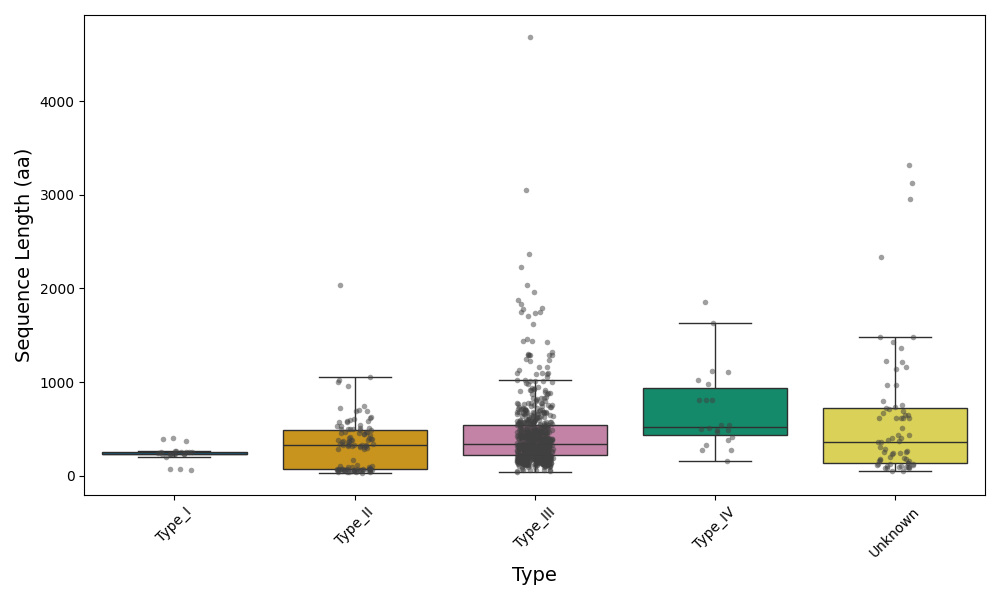
\includegraphics[width=0.9\textwidth]{images/sequence_length_by_type.png} 
		\caption{\textbf{Sequence length distribution for different bacterial exotoxin types.}(measured in amino acids).
			The x-axis represents the exotoxin types and each toxin type is represented by a distinct colors: Type I (yellow), Type II (orange), Type III (pink), Type IV (green), and Unknown (yellow). 
			The y-axis shows sequence length in amino acids, ranging from 0 to approximately 3000 except three outliers.}
		\label{fig:sequence_length_by_type}
	\end{subfigure}
	\vspace{1em}
	\begin{subfigure}{\textwidth}
		\centering
		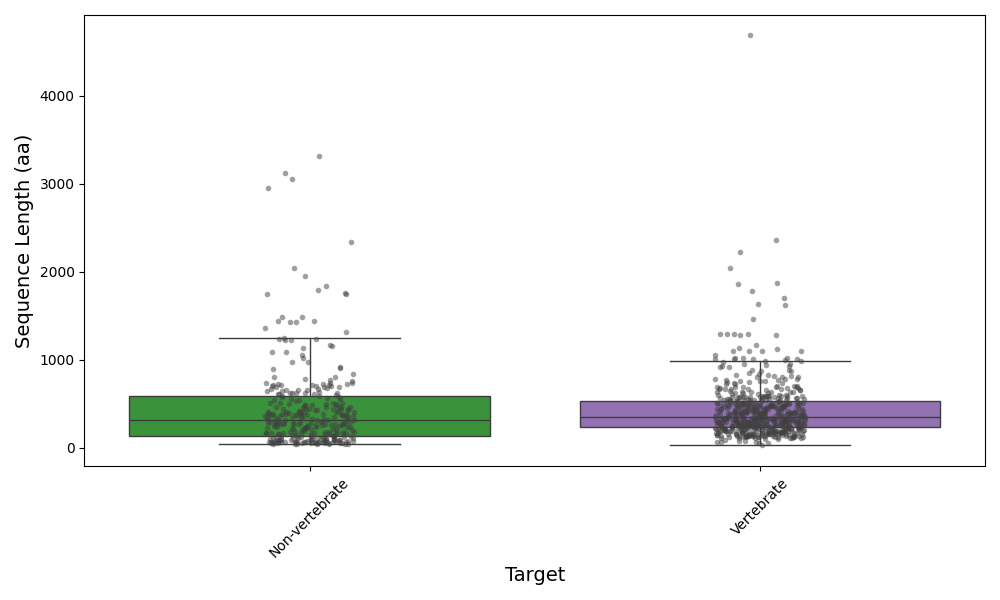
\includegraphics[width=0.9\textwidth]{images/sequence_length_by_target.png}
		\caption{\textbf{Sequence length distribution for different bacterial exotoxin targets.}(measured in amino acids).
			The x-axis represents the exotoxin targets, and each toxin type is represented by a distinct color: Vertebrates (dark green) and Non-vertebrates (purple).
			The y-axis shows sequence length in amino acids, ranging from 0 to approximately 2500 except five outliers.}
		\label{fig:sequence_length_by_target}
	\end{subfigure}
	\caption{Descriptive Analysis of Bacterial Exotoxin Feature: Sequence Length}
\end{figure}

\begin{figure}[h]
	\centering
	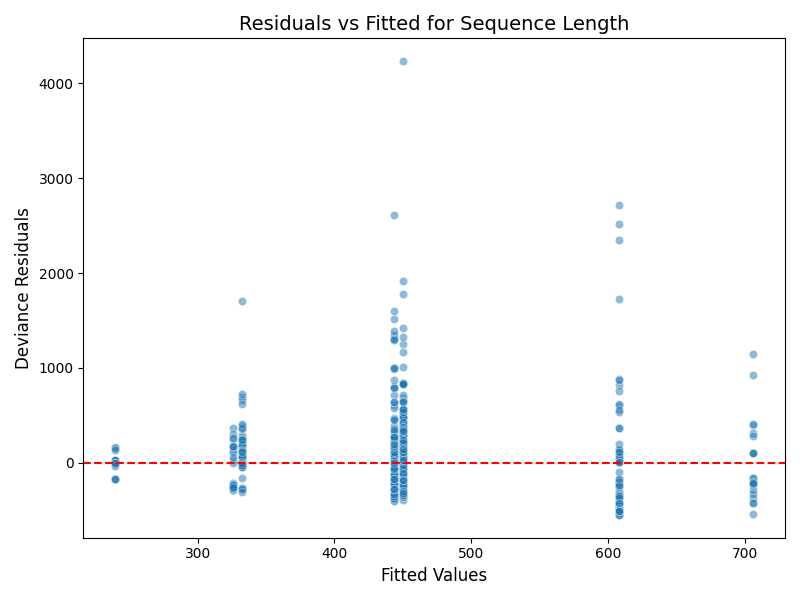
\includegraphics[width=0.7\textwidth]{images/residuals_sequence_length_deviance.png}
	\caption{Deviance residuals vs. fitted values for the GLM on sequence length. Large residuals indicate that the model does not fully capture the variance in sequence length, suggesting that additional factors influence sequence length beyond toxin type.}
	\label{fig:res_seq_length}
\end{figure}

The residuals plot shows large deviations, meaning that the model struggles to explain the variance in sequence length. This suggests that sequence length alone does not fully account for the differentiating between toxin types.

\subsubsection{Hydrophobicity Feature Analysis}
\begin{figure}[H]
	\centering
	\begin{subfigure}[b]{\textwidth}
		\centering
		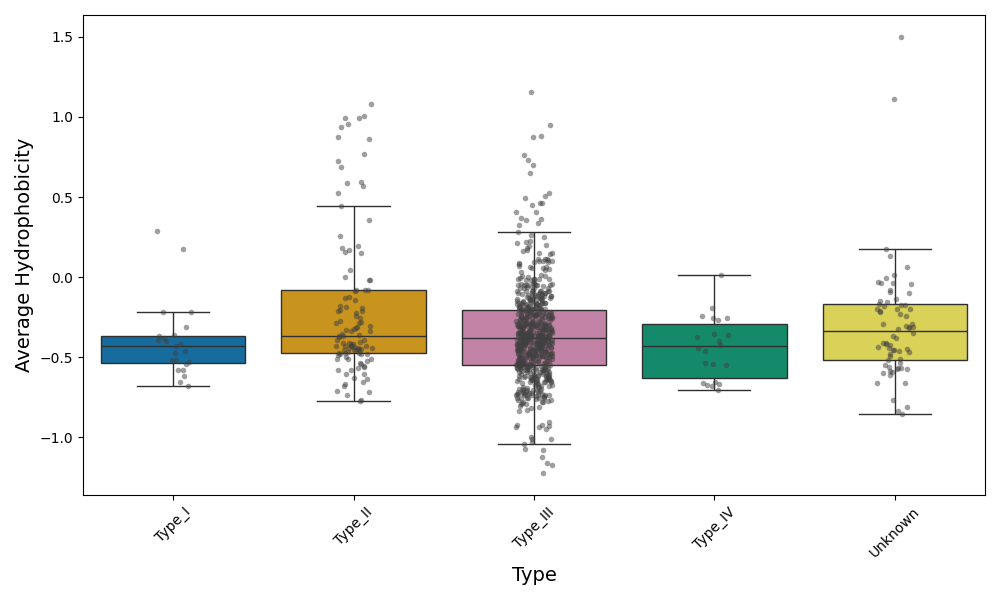
\includegraphics[width=0.9\textwidth]{images/hydrophobicity_by_type.png} % Replace with your figure file
		\caption{\textbf{Hydrophobicity distribution for different bacterial exotoxin types.}(measured in amino acids).
			The x-axis represents the exotoxin types and each toxin type is represented by a distinct color: Type I (blue), Type II (orange), Type III (pink), Type IV (green), and Unknown (yellow). The y-axis shows the average hydrophobicity values, ranging from approximately -1.5 to 1.0. Each box plot displays the median hydrophobicity, interquartile range (IQR), and whiskers extending up to 1.5 times the IQR. Individual outliers are marked as points outside the whiskers. The hydrophobicity values vary slightly across toxin types, with Type II showing a wider spread compared to others, while Type I and Type IV are more compact.}
		\label{fig:hydrophobicity_toxin_type}
	\end{subfigure}
	\vspace{1em}
	\begin{subfigure}{\textwidth}
		\centering
		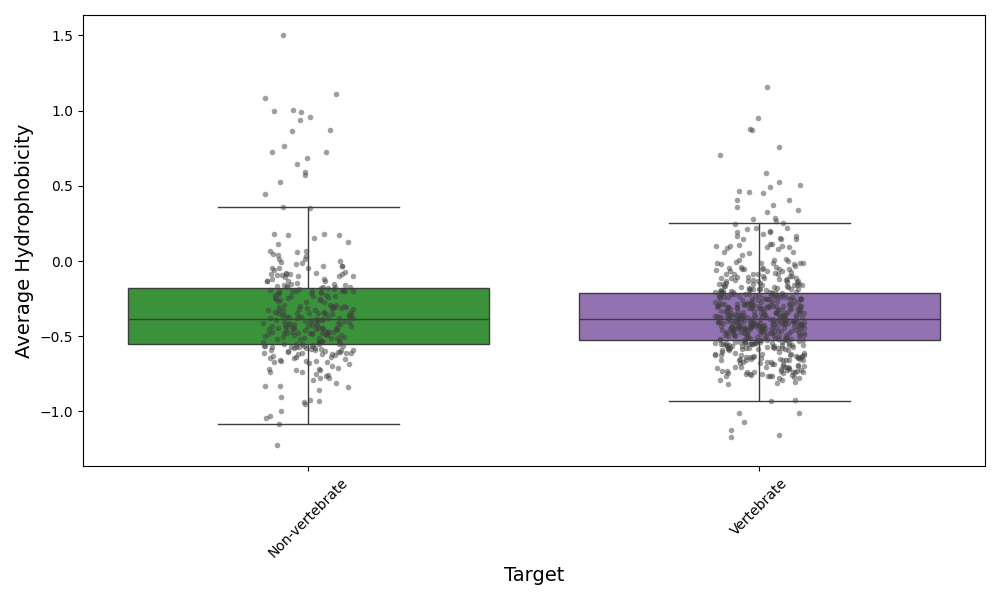
\includegraphics[width=0.9\textwidth]{images/hydrophobicity_by_target.png} 
		\caption{\textbf{Hydrophobicity distribution for different bacterial exotoxin targets.}(measured in amino acids).
			The x-axis represents the exotoxin targets, and each toxin target is represented by a distinct color: Vertebrates (dark green) and Non-vertebrates (purple).
			The y-axis shows the average hydrophobicity values, ranging from approximately -1.5 to 1.0. Each box plot summarizes the data, showing the median hydrophobicity, interquartile range (IQR), and whiskers extending up to 1.5 times the IQR, with outliers plotted as individual points. Both vertebrate and non-vertebrate targets have similar distributions, but vertebrate targets exhibit a slightly wider variation in hydrophobicity compared to non-vertebrate targets.}
		\label{fig:hydrophobicity_by_target}
	\end{subfigure}
	\caption{Descriptive Analysis of Bacterial Exotoxin Feature: Hydrophobicity}
\end{figure}

The boxplot analysis investigated whether hydrophobicity introduce biases. Using Generalized Linear Models (GLMs), we found that Type II toxins have significantly higher hydrophobicity, with a coefficient of 0.2075 (p = 0.007), meaning their hydrophobicity is 0.2075 units higher on average compared to the reference category. In contrast, Type III, Type IV, Unknown toxins, and vertebrate-targeting toxins showed no significant effect on hydrophobicity (p > 0.05), suggesting similar hydrophobicity levels across these groups. Since only Type II toxins exhibit a significant increase, this could introduce a bias in predictive models that use hydrophobicity as a feature.

\begin{figure}[h]
	\centering
	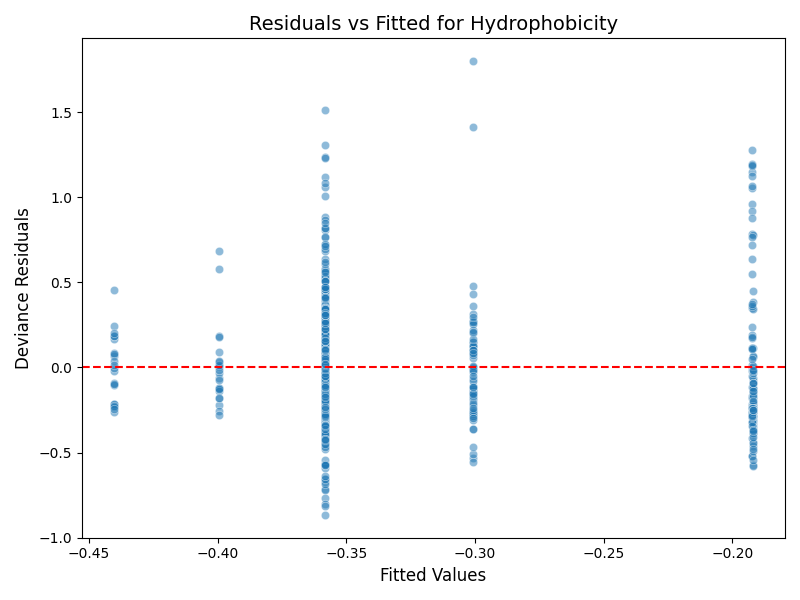
\includegraphics[width=0.7\textwidth]{images/residuals_hydrophobicity_deviance.png}
	\caption{Deviance residuals vs. fitted values for the GLM on hydrophobicity. The scattered residuals suggest that toxin type alone does not strongly predict hydrophobicity, indicating the need for additional explanatory variables.}
	\label{fig:res_seq_hydro}
\end{figure}

As shown in Figure~\ref{fig:res_seq_hydro}, the residuals plot demonstrates that hydrophobicity does not show a strong pattern across toxin types. The scattered points and presence of high residuals indicate unexplained variance, meaning that additional biochemical properties may be influencing hydrophobicity.

\subsection{Quality of Protein Folds Based On pLDDT Scores}

In Figure~\ref{fig:lddt_scores}, the predicted Local Distance Difference Test values that were gathered from the scores from the B-factor column of each residue were plotted in a distribution plot.

The increasing LDDT scores across targets indicate higher confidence in the targets with higher numbers, while greater variability in lower scores could indicate further analysis in terms of prediction accuracy. 

\begin{figure}[H]
	\centering
	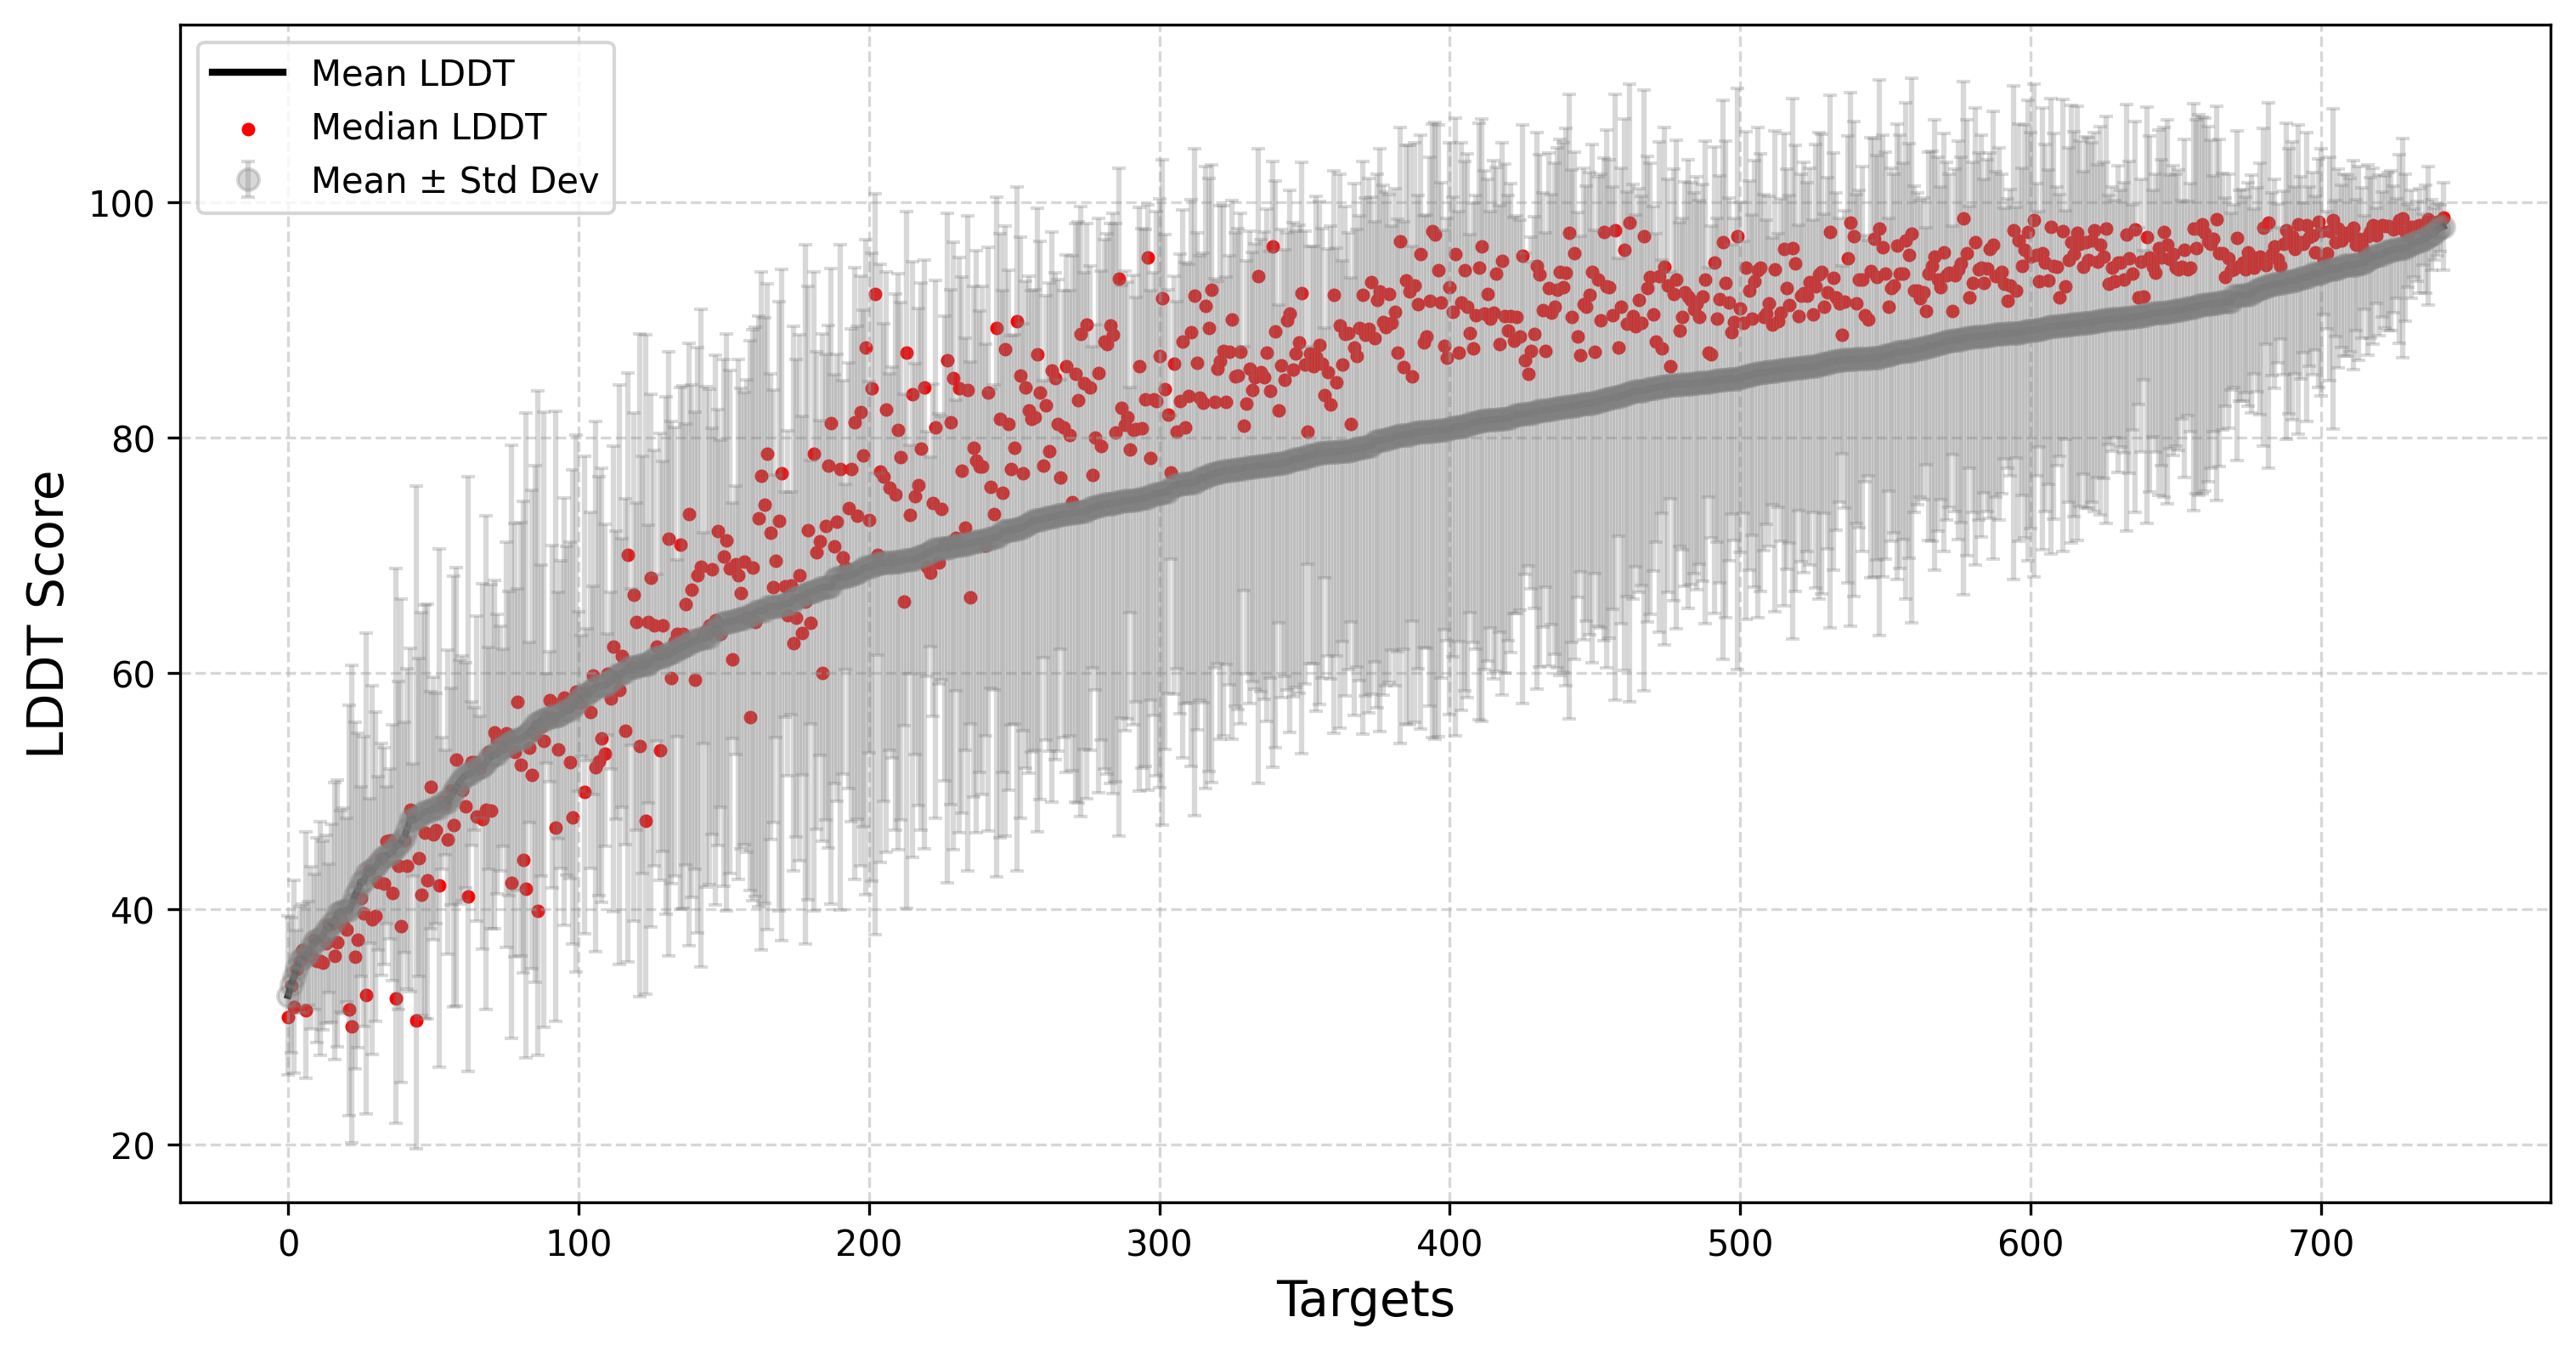
\includegraphics[width=0.9\textwidth]{images/LDDT.png}
	\caption{LDDT Score Distribution Across Targets. The black line represents the mean LDDT score for each target, while the gray error bars indicate the standard deviation. Red points denote the median LDDT score for each target. This visualization highlights the distribution of model confidence across different protein structures. Low-confidence predictions correspond to LDDT< 50, high confidence regions correspond to LDDT > 70.}
	\label{fig:lddt_scores}
\end{figure}

\pagebreak

\subsection{Dimensionality Reduction Techniques}

Principal Component Analysis (PCA) was applied to both the standard and scrambled datasets to assess the separation of vertebrate and non-vertebrate sequences. In the target PCA, vertebrates colored in purple and non-vertebrates colored in dark green show some clustering, suggesting biologically meaningful features, though with overlap. 

In Figure~\ref{fig:pca_toxin_type}, PCA plot for exotoxin types, Type II and Type IV showed distinct clustering, whereas Type III is scattered randomly with small clustering among its groups, often between 0 and 0.75 on the Principal Component 1 axis. However, there is clear overlapping among data points of different types between -0.75 and 0 on the Principal Component 1 axis which indicates there might be difficulties in classifying them accurately.

In contrast, in Figure~\ref{fig:scrambled_pca_toxin_type}, the scrambled PCA lacks any visible structure, confirming that the patterns in the target PCA are in fact meaningful. This validates that the learned features effectively capture relevant biological information.

\begin{figure}[H]
	\centering
	\begin{subfigure}{\textwidth}

		\centering
		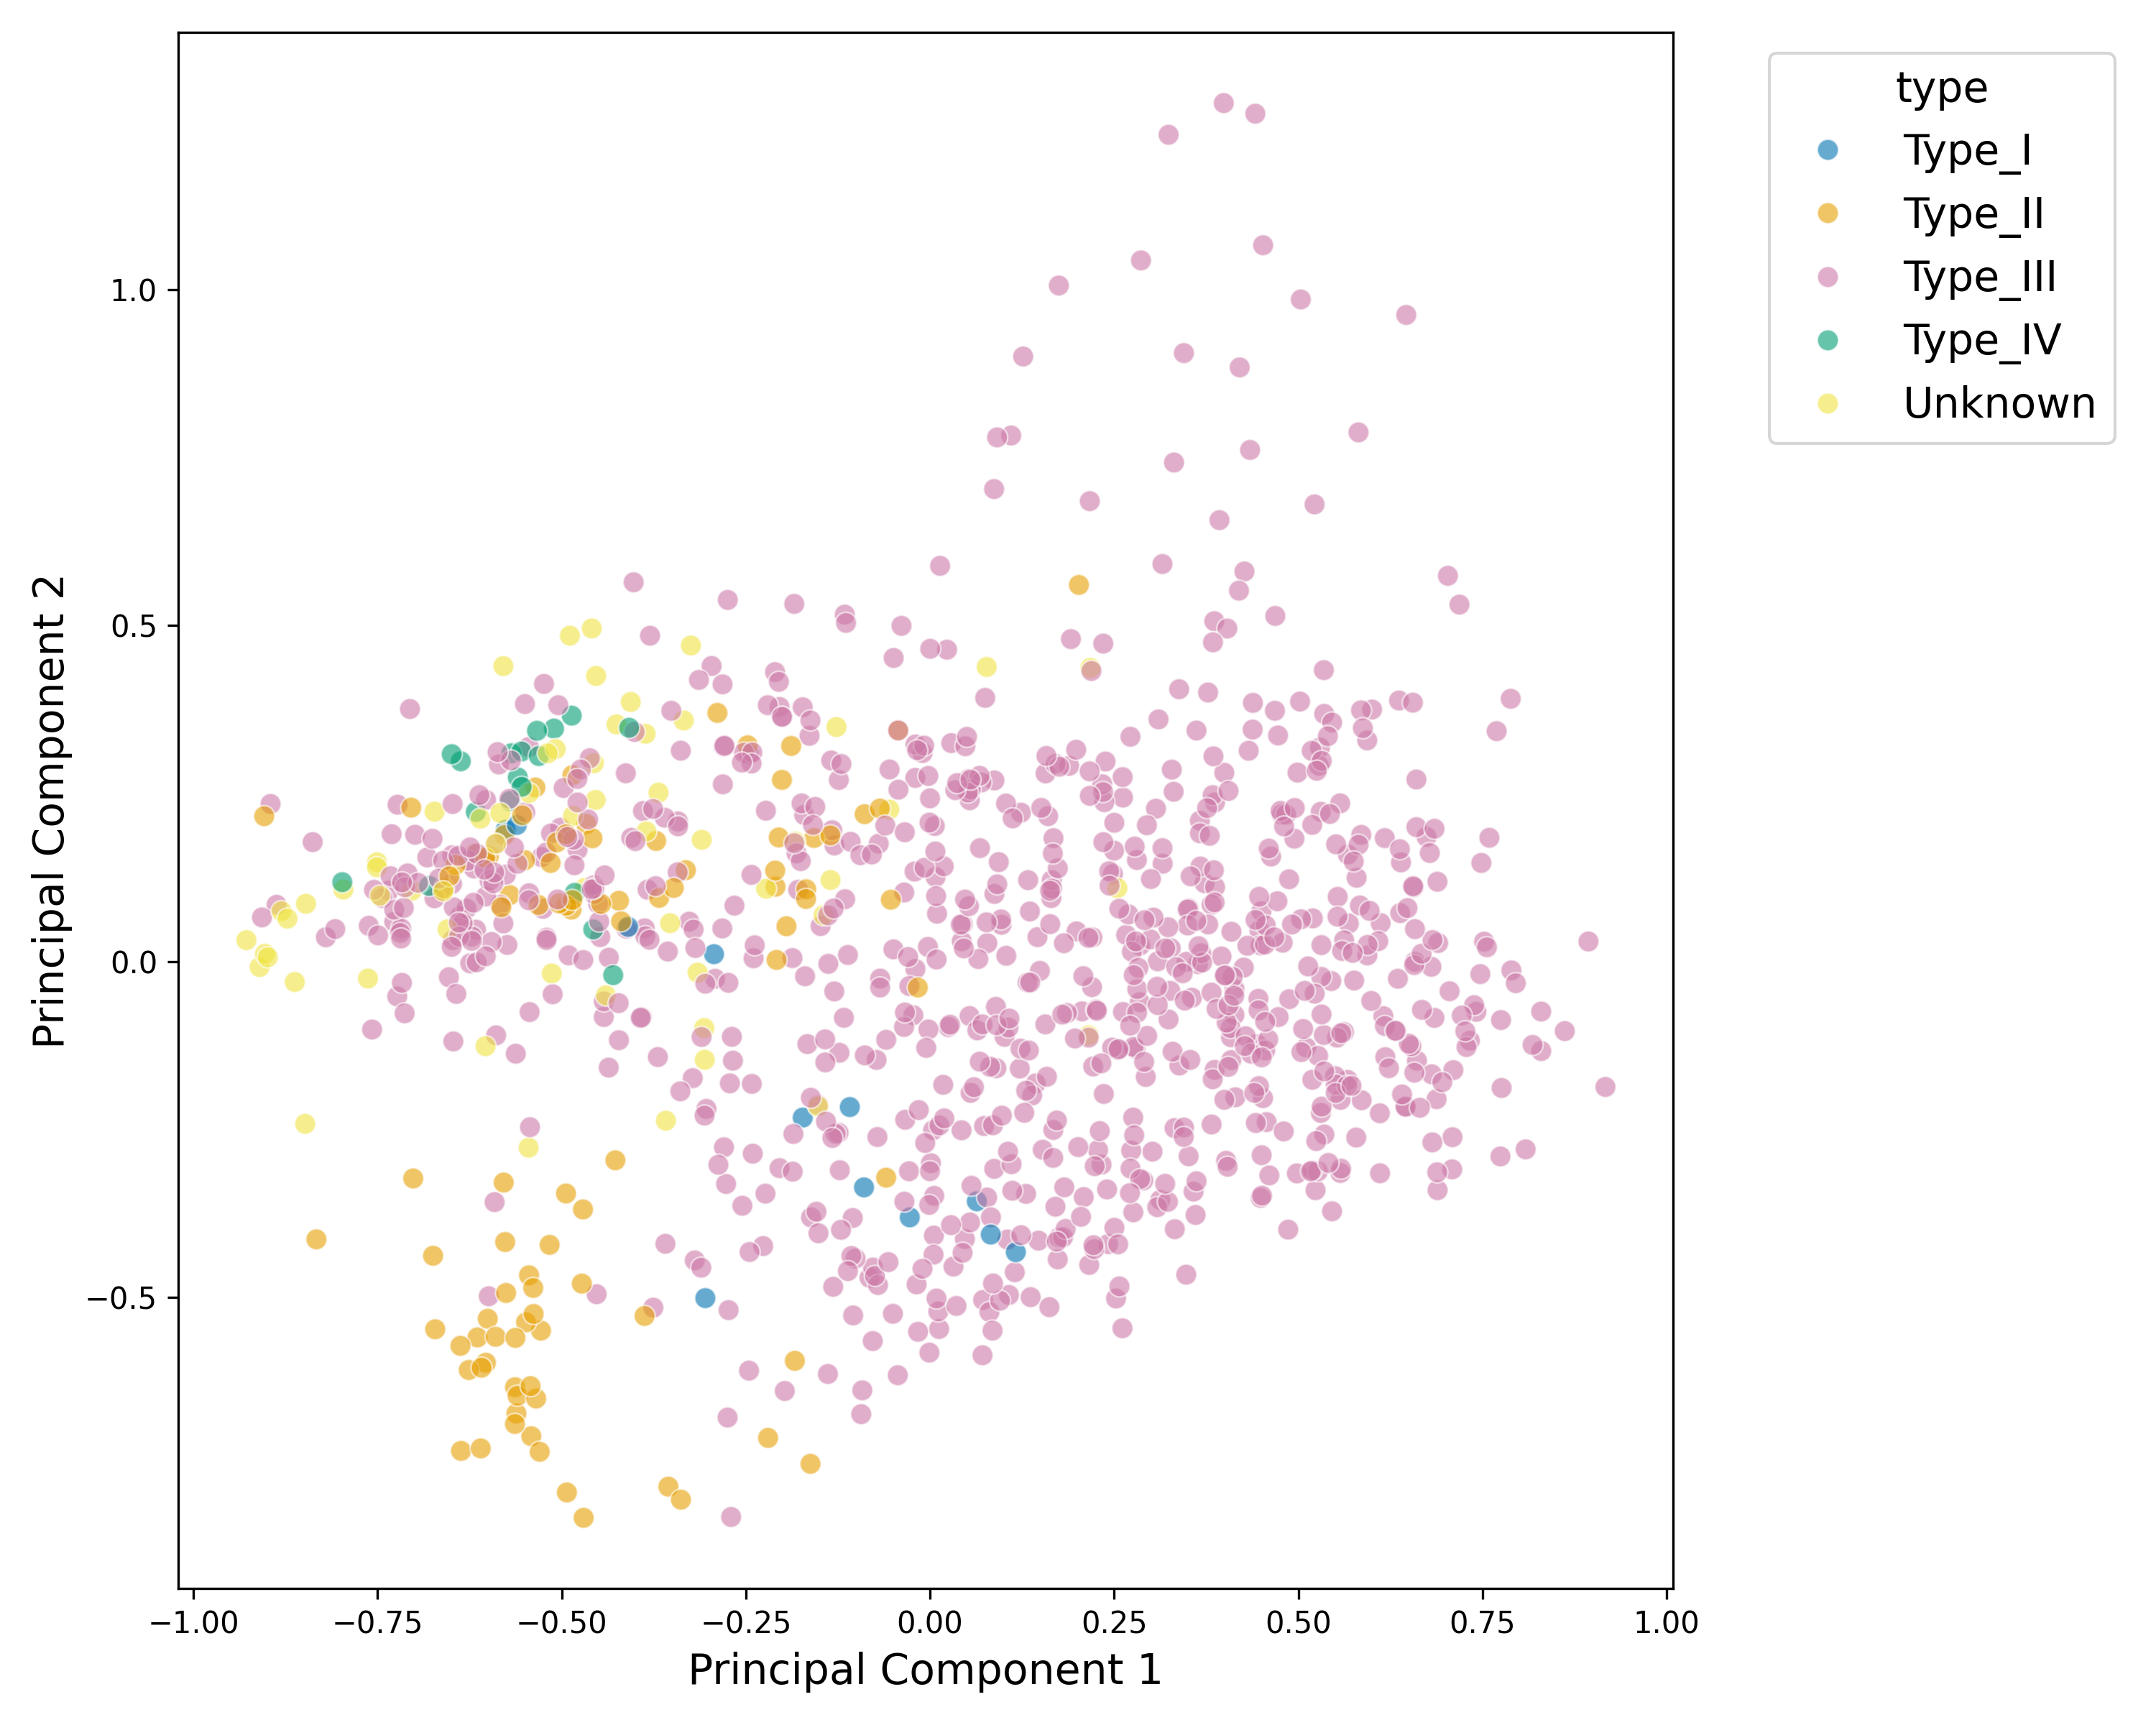
\includegraphics[width=0.7\textwidth]{images/pca_projection_type.png} 
		\caption{\textbf{Principal Component Analysis (PCA) projection of bacterial exotoxin types}
			The x-axis represents Principal Component 1, and the y-axis represents Principal Component 2, both ranging from approximately -1.0 to 1.0. Each exotoxin type is color-coded: Type I (blue), Type II (purple), Type III (pink), Type IV (green), and Unknown (yellow). Clusters suggest some overlap but distinct separations for specific types.}
		\label{fig:pca_toxin_type}
	\end{subfigure}
	\vspace{1em}
	\begin{subfigure}{\textwidth}
		\centering
		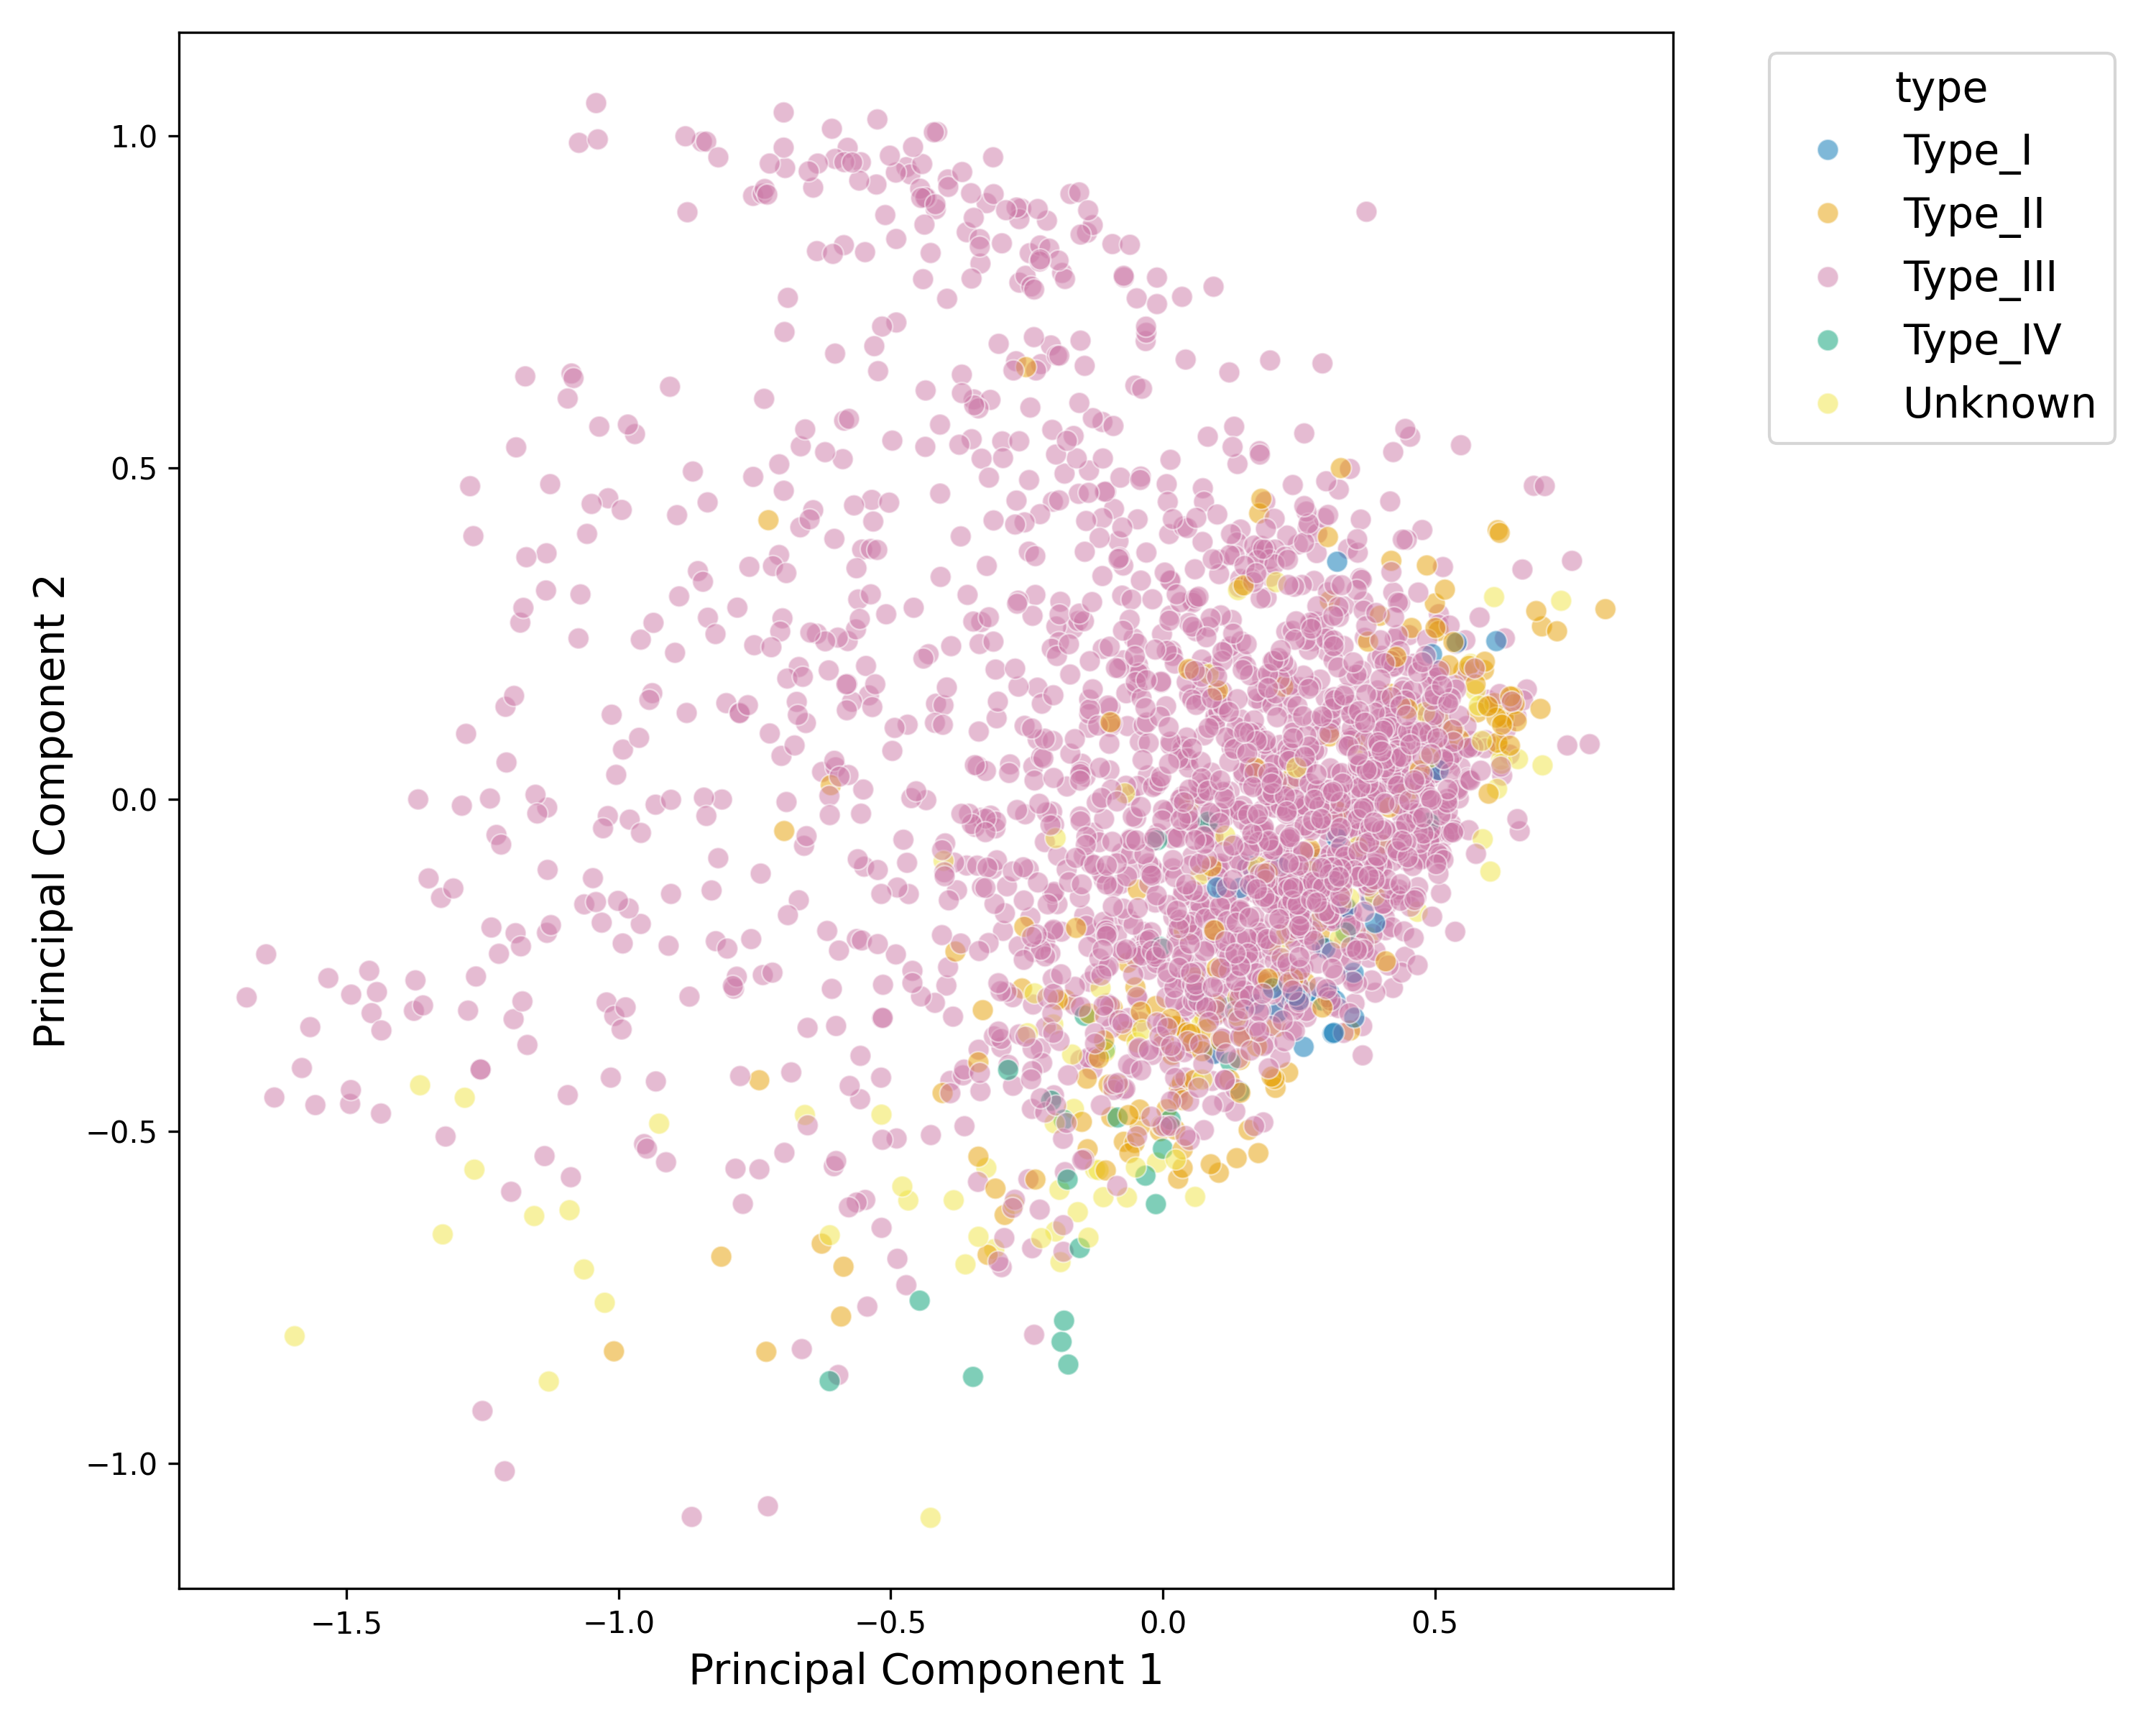
\includegraphics[width=0.7\textwidth]{images/pca_projection_type_scrambled.png} 
		\caption{Scrambled PCA projection of bacterial exotoxin types.The x-axis represents Principal Component 1, and the y-axis represents Principal Component 2, with a wider range of values between -1.5 and 1.0. The same color coding applies:Type I (blue), Type II (purple), Type III (pink), Type IV (green), and Unknown (yellow). The scrambling reduces separation among the clusters, validating the effect of shuffling of protein sequences.}
		\label{fig:scrambled_pca_toxin_type}
	\end{subfigure}
	\caption{Principal Component Analysis Based On Exotoxin Types For Dimensionality Reduction}
	\label{fig:dimensionality_reduction_toxin_type}
\end{figure}

\begin{figure}[H]
	\centering
	\begin{subfigure}[b]{\textwidth}
		\centering
		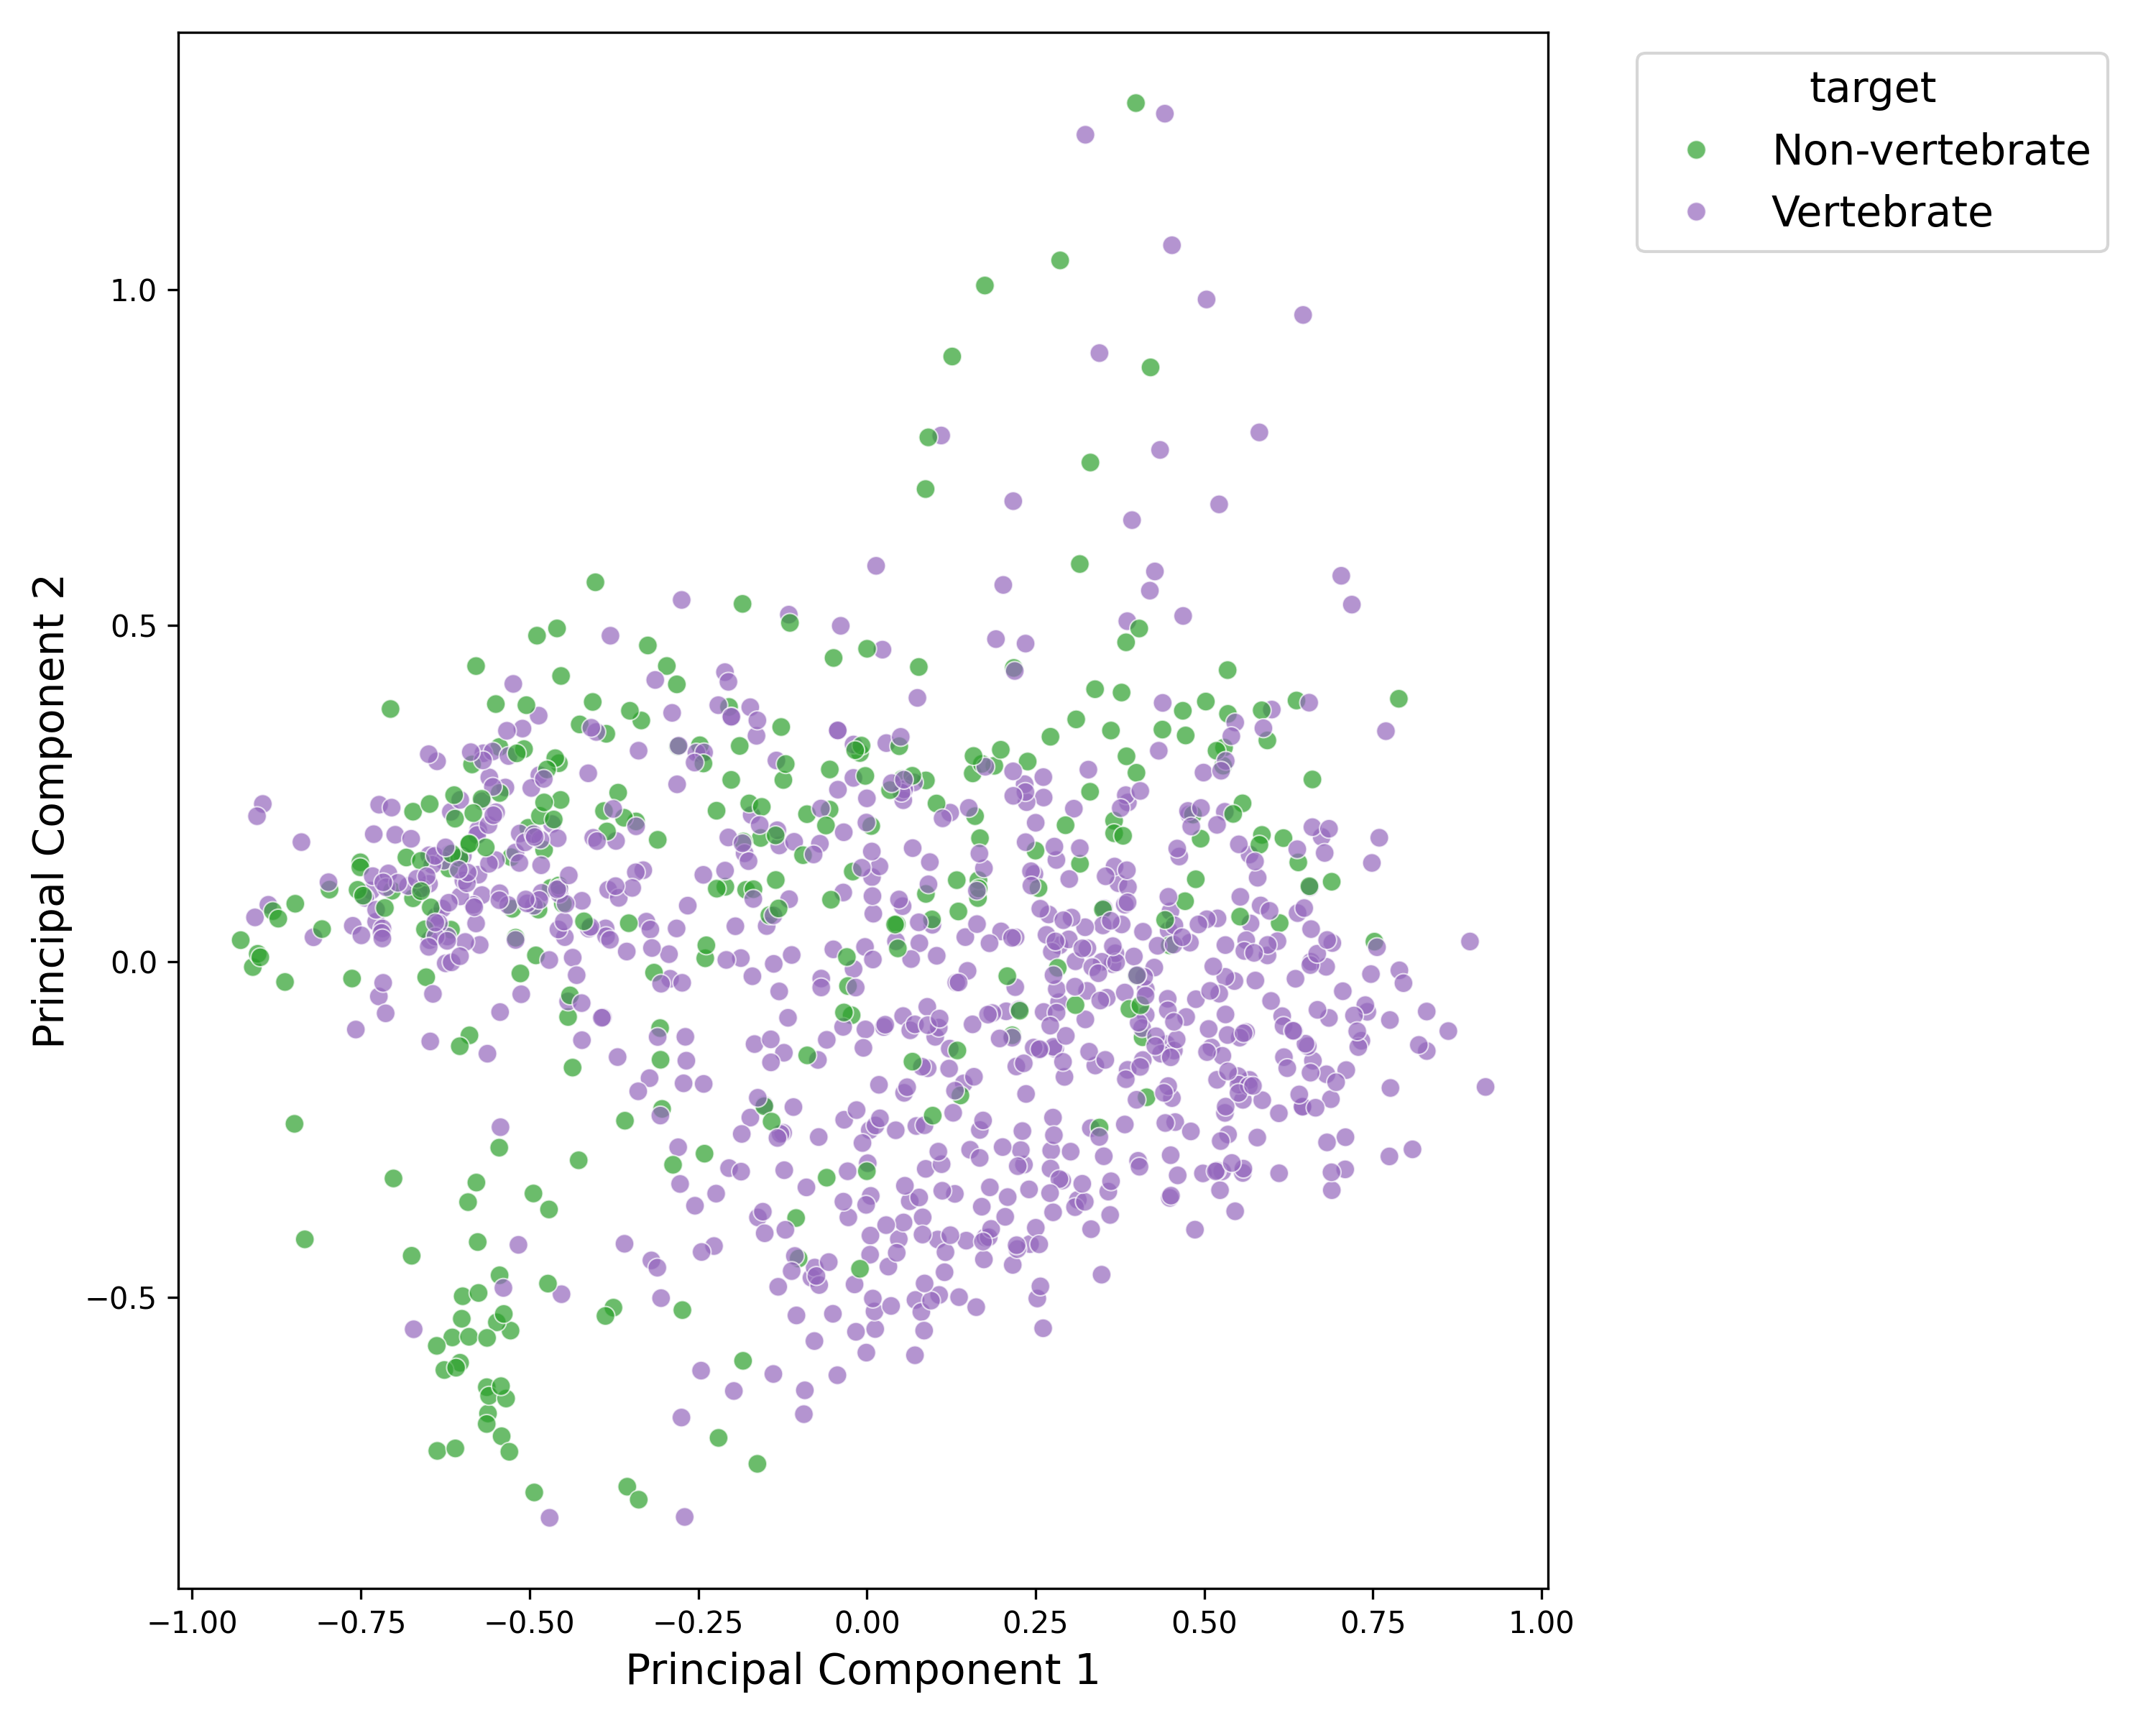
\includegraphics[width=0.7\textwidth]{images/pca_projection_target.png} 
		\caption{Principal Component Analysis (PCA) projection of bacterial exotoxin targets.The x-axis represents Principal Component 1, and the y-axis represents Principal Component 2, both ranging from approximately -1.0 to 1.0. Targets are color-coded: Vertebrates (purple) and Non-vertebrates (dark green). Vertebrate clusters are more compact, while non-vertebrate clusters show broader variability.}
		\label{fig:pca_projection_non_scrambled_target}
	\end{subfigure}
	\vspace{1em}
	\begin{subfigure}[b]{\textwidth}
		\centering
		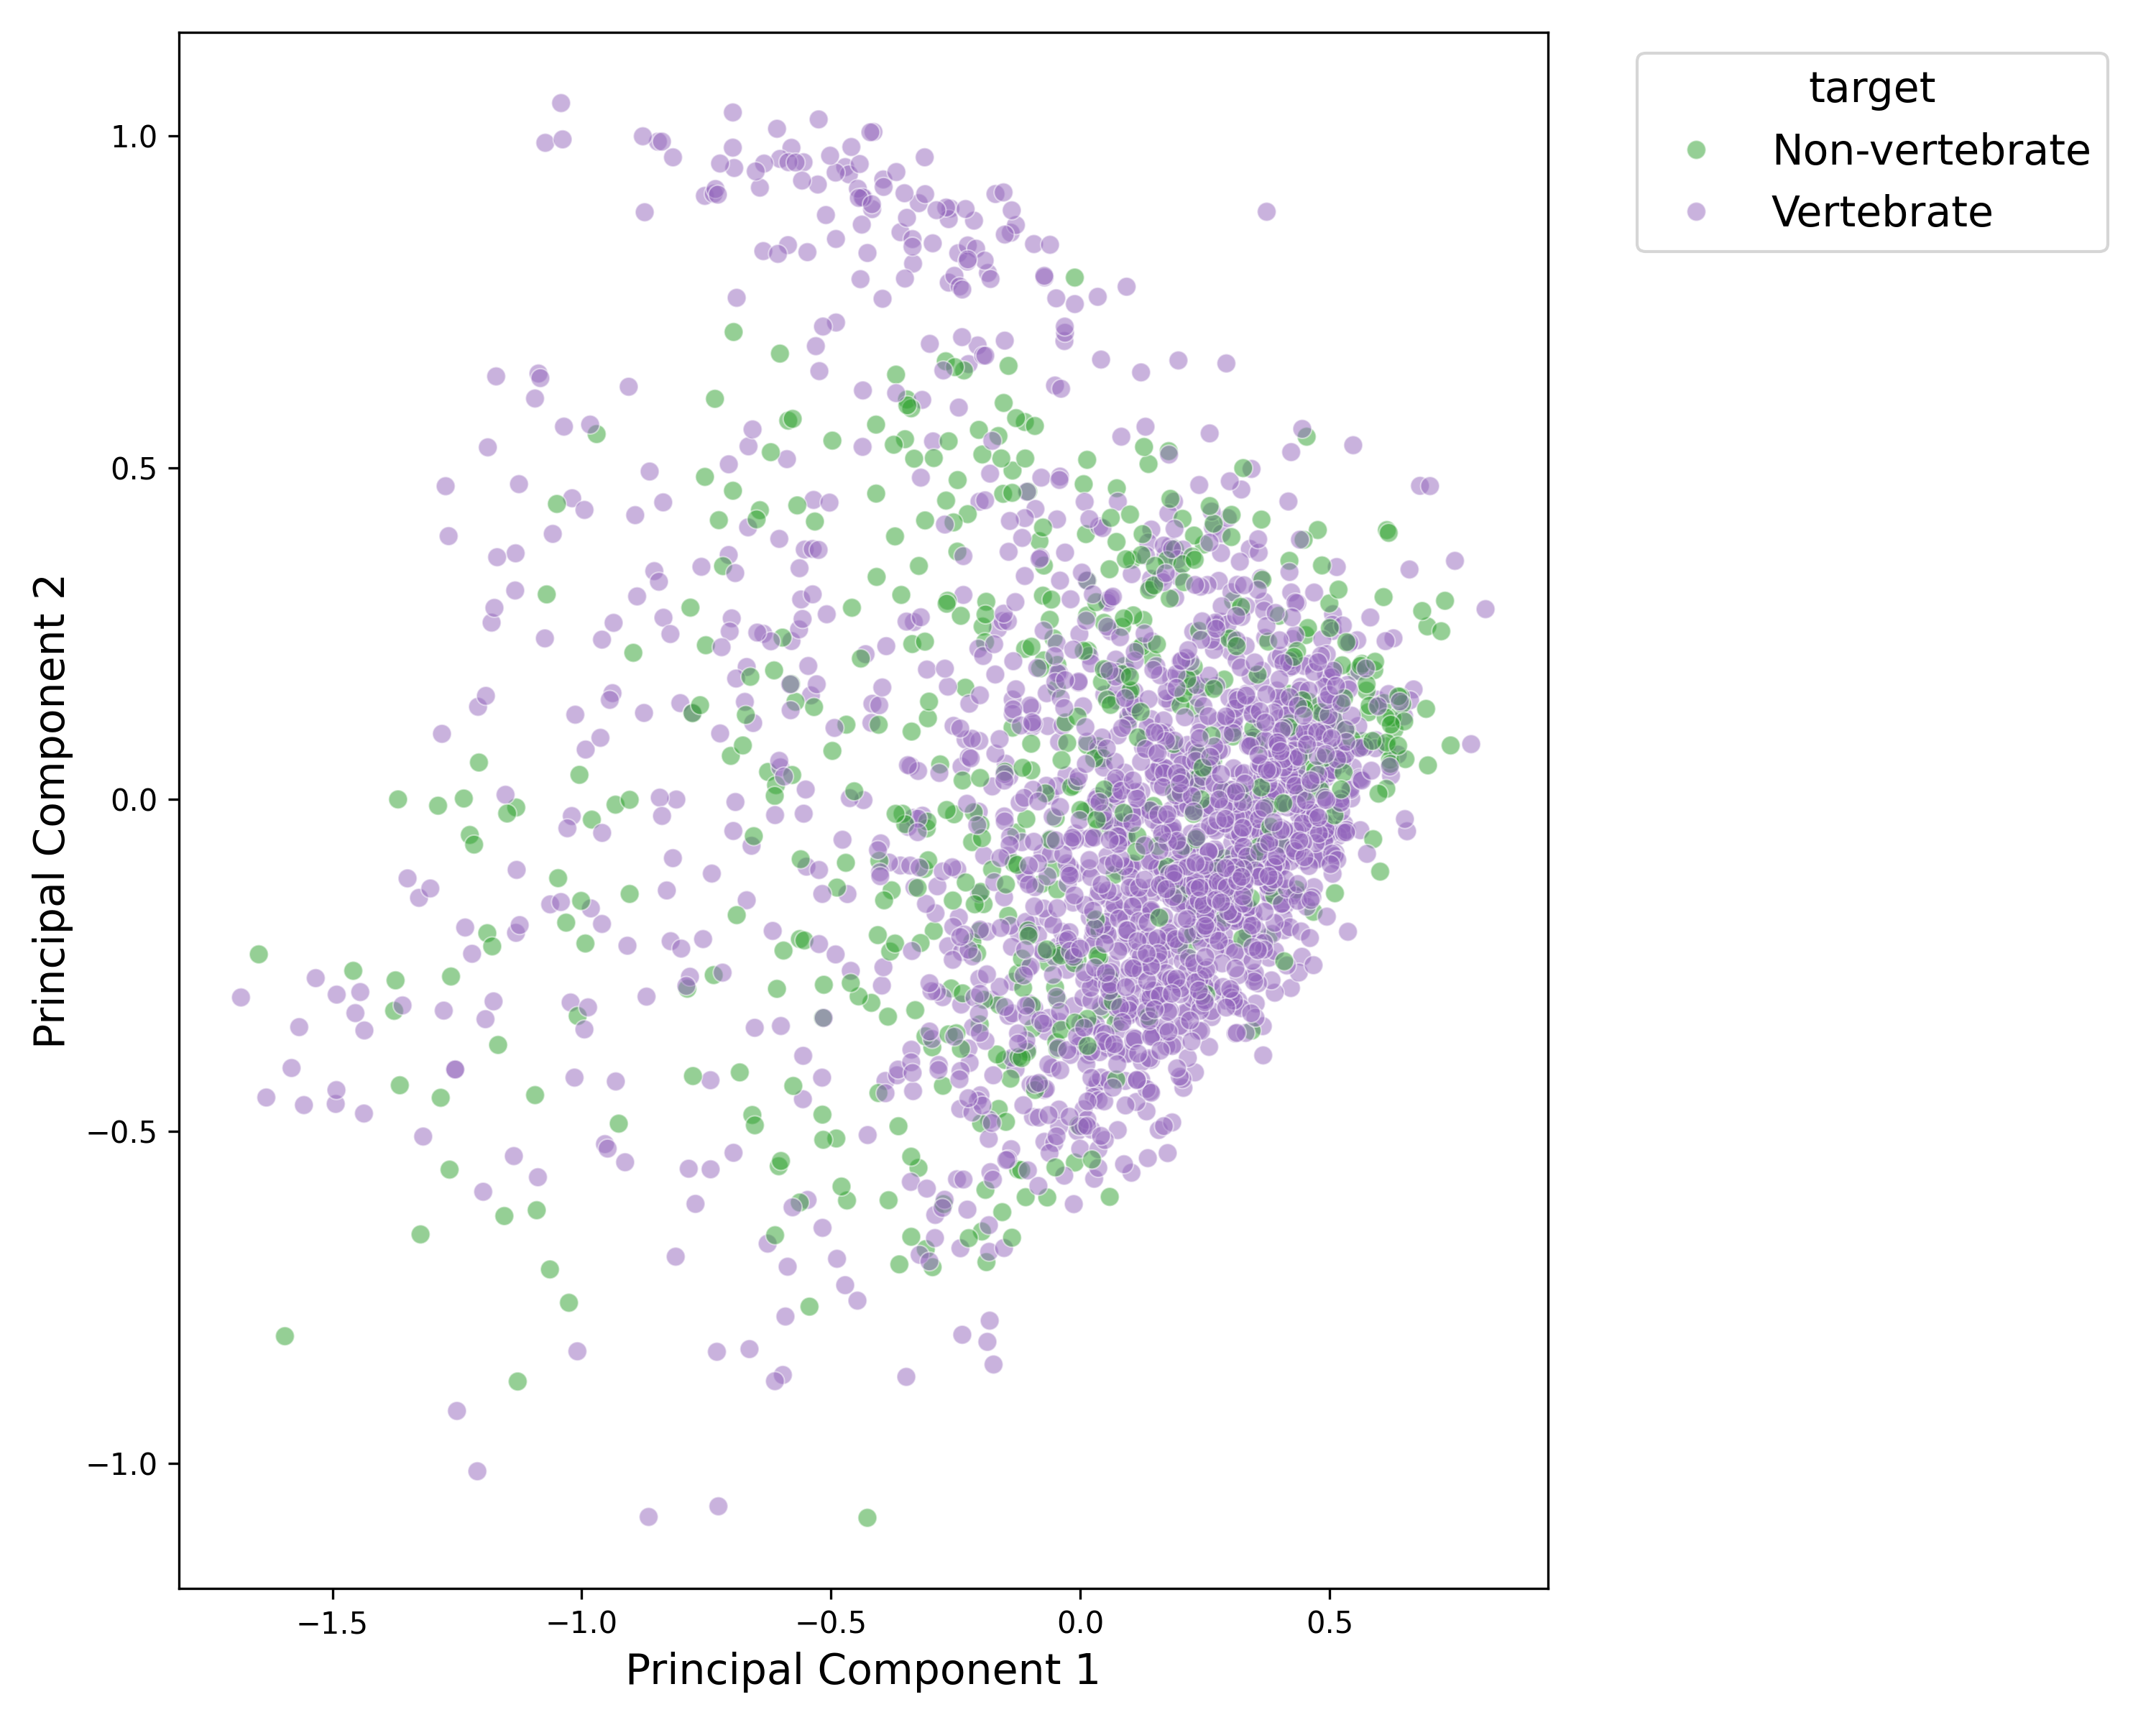
\includegraphics[width=0.7\textwidth]{images/pca_projection_target_scrambled.png}
		\caption{Scrambled PCA projection of bacterial exotoxin targets.The x-axis represents Principal Component 1, and the y-axis represents Principal Component 2, with a wider range of values (-1.5 to 1.0). Targets are color-coded as Vertebrates (orange) and Non-vertebrates (blue). The scrambling reduces cluster compactness, demonstrating the loss of structure in the data.}
		\label{fig:pca_projection_scrambled_target}
	\end{subfigure}
	\caption{Principal Component Analysis Based On Exotoxin Targets For Dimensionality Reduction}
	\label{fig:dimensionality_reduction_toxin_target}
\end{figure} 

\subsection{ExoType Predictor}

This section explains the steps taken to build the best-performing machine learning classification model. The predictor, called ExoType, differentiates bacterial exotoxins into five categories: Type I, Type II, Type III, Type IV, and Unknown (representing other exotoxin types that have not been classified yet). This part describes the training and validation process, along with the evaluation of model performance, leading to the final model selection.

\subsection{Model Training}

To ensure robust model evaluation and mitigate class imbalance,  5-fold cross-validation was employed with class\_weight=balanced and GridSearchCV for hyperparameter tuning. 

In the beginning of the training process, the preprocessed dataset was splitted into a 80\%-20\% training-test split, ensuring that the overall dataset contained only non-redundant data. This approach aimed to evaluate the models’ ability to generalize to truly novel sequences. However, due to the naturally uneven distribution of exotoxin classes, the limited sample size in certain exotoxin classes resulted in higher variance. For example,  KNN and Logistic Regression models indicated overfitting in Figure~\ref{fig:split_test_learning_curves} with the training curve being a straight line.

In the second approach, the entire non-redundant dataset was used for training, while the previously eliminated redundant sequences formed the test set. In this Figure~\ref{fig:import_test_learning_curves}, KNN and Logistic Regression performed better than in the first approach, likely due to the increased training data, while Random Forest and SVM still maintained strong performance with smooth and well-aligned learning curves with a reduction in overfitting and more alignment of training/validation curves during training.

\subsubsection{Learning Curves for Protein Sequence-Based Embeddings}

While the first approach displays a more traditional generalization test, the second approach benefits from a richer training set at the cost of testing on potentially redundant data. Random Forest and SVM performed well in both cases, but the first approach led to greater variability in KNN and Logistic Regression, making them less reliable for handling unseen data. 

\begin{figure}[H]
	\centering
	\begin{subfigure}[b]{0.9\textwidth}
		\centering
		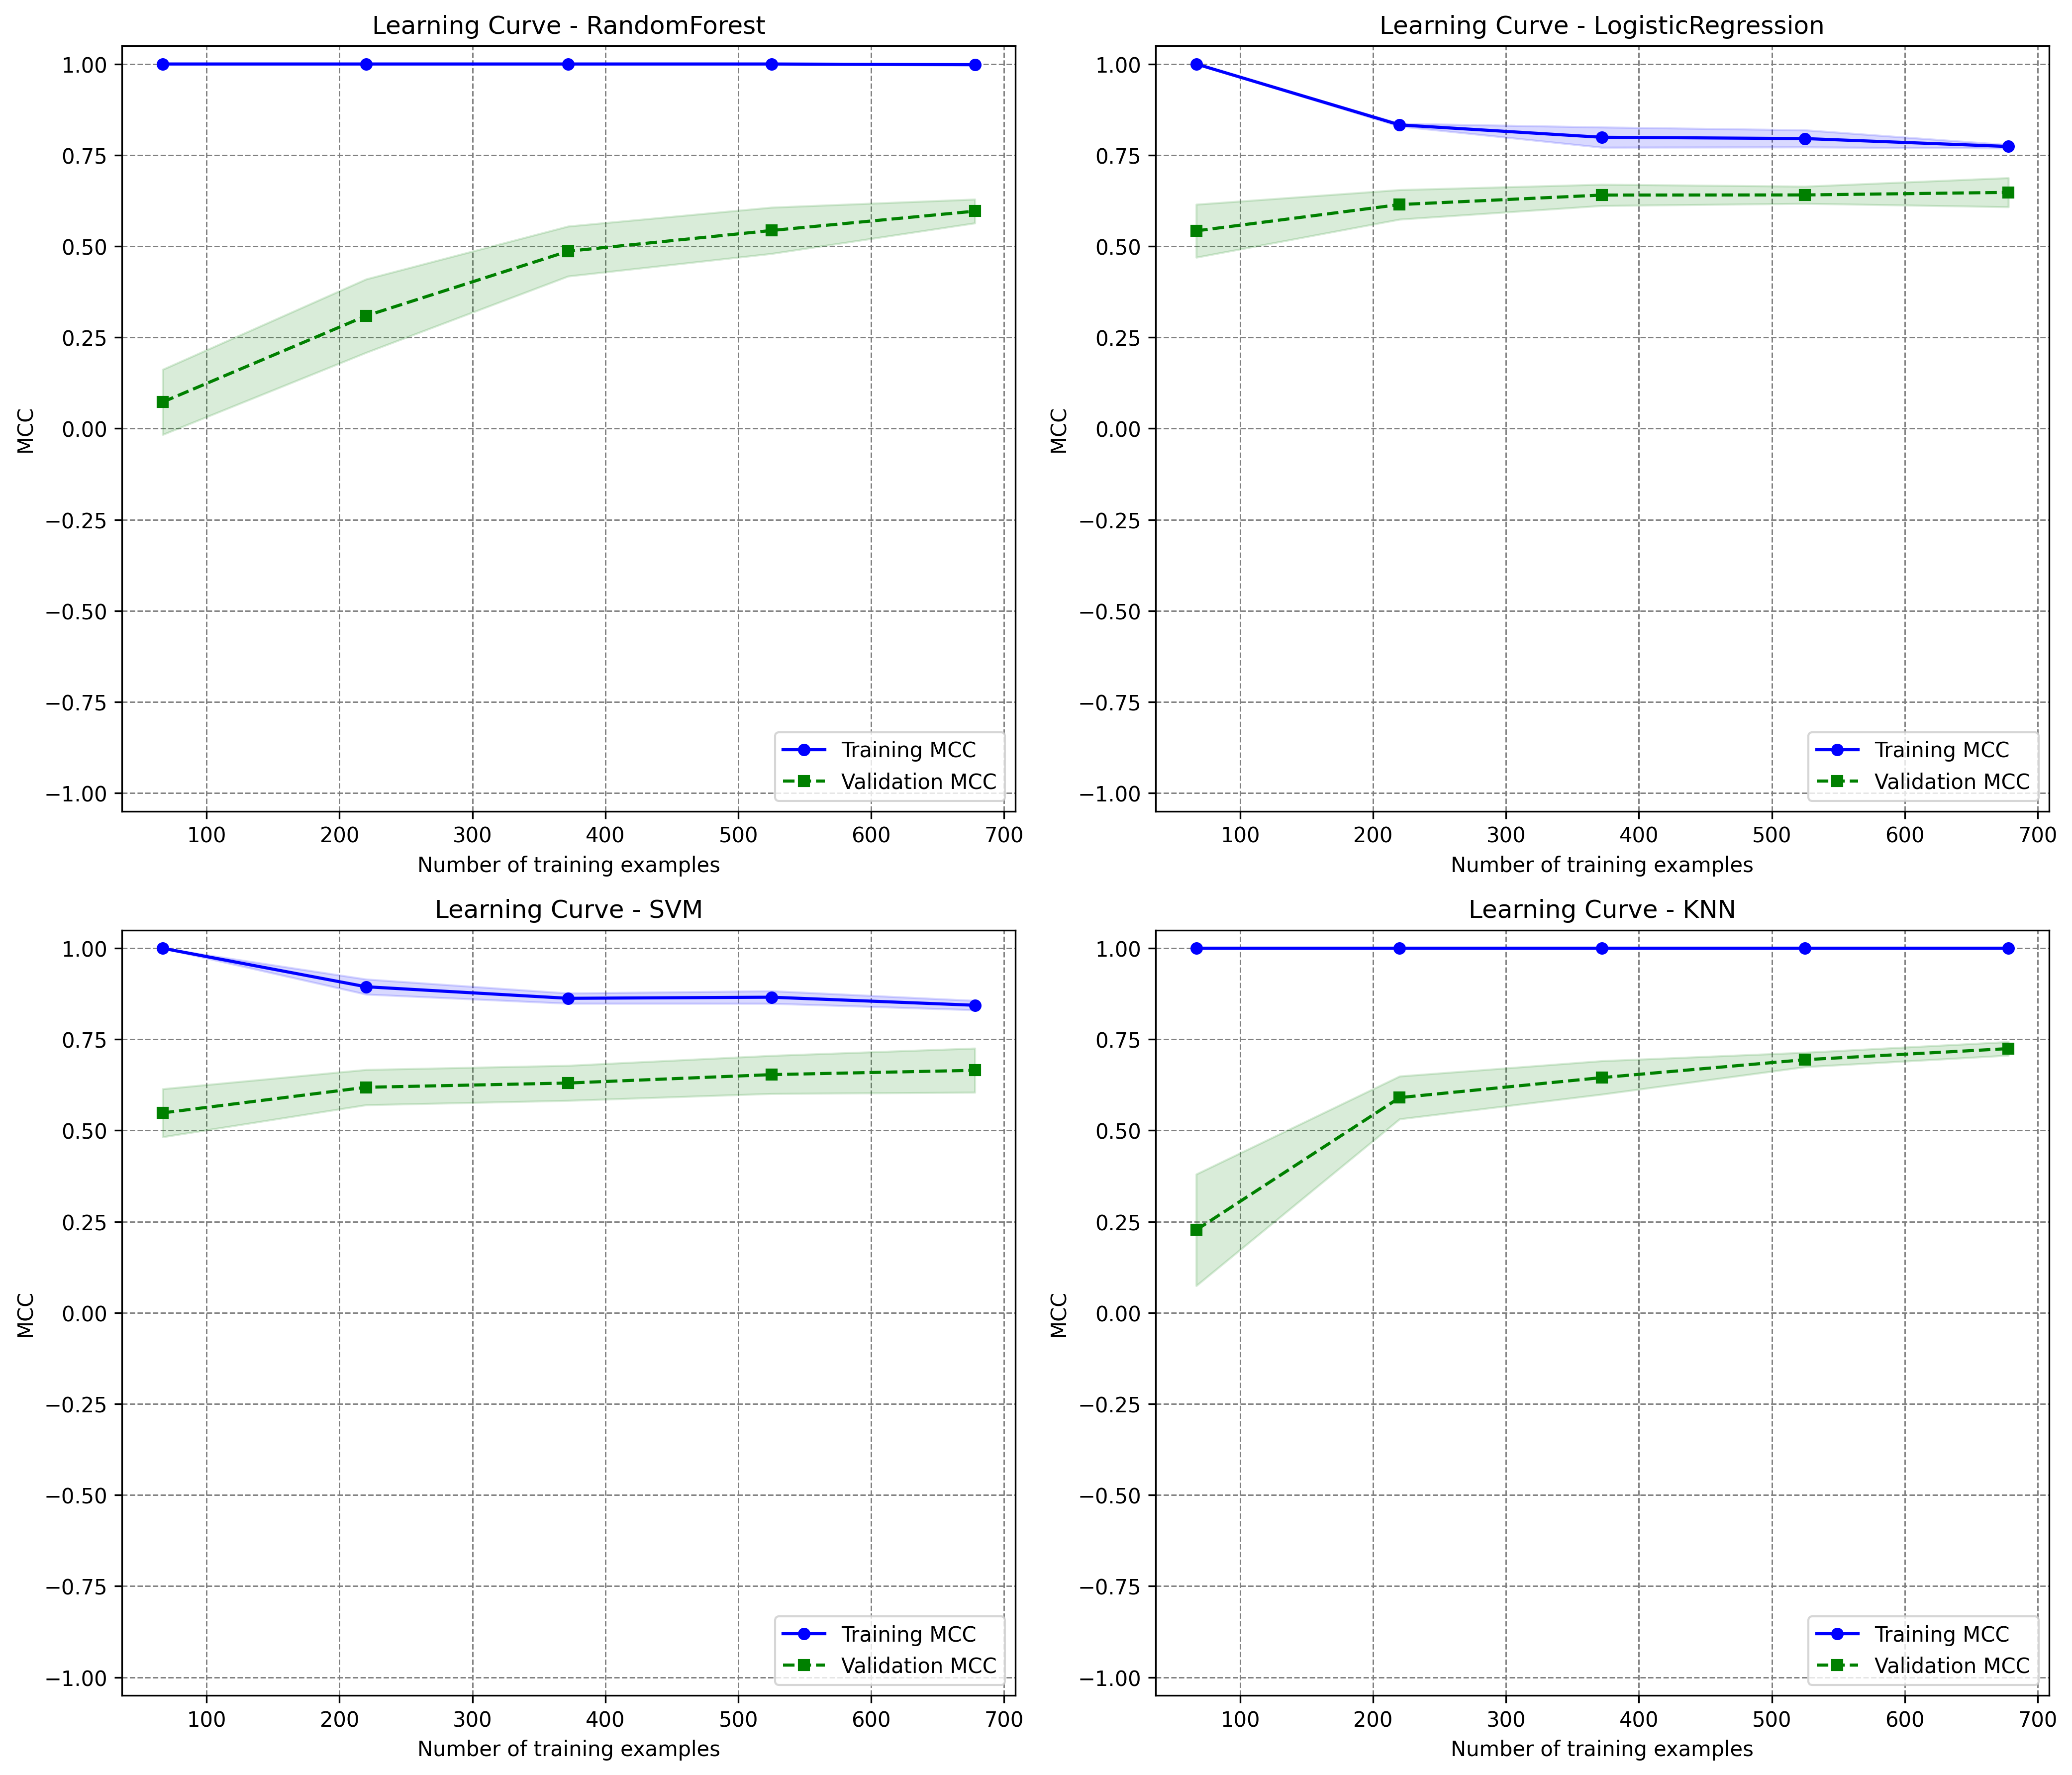
\includegraphics[width=\textwidth]{images/2x2_learning_curves_split_test_type.png}
		\caption{Learning Curves - Split Test Type}
		\label{fig:split_test_learning_curves}
	\end{subfigure}
	
	\begin{subfigure}[b]{0.9\textwidth}
		\centering
		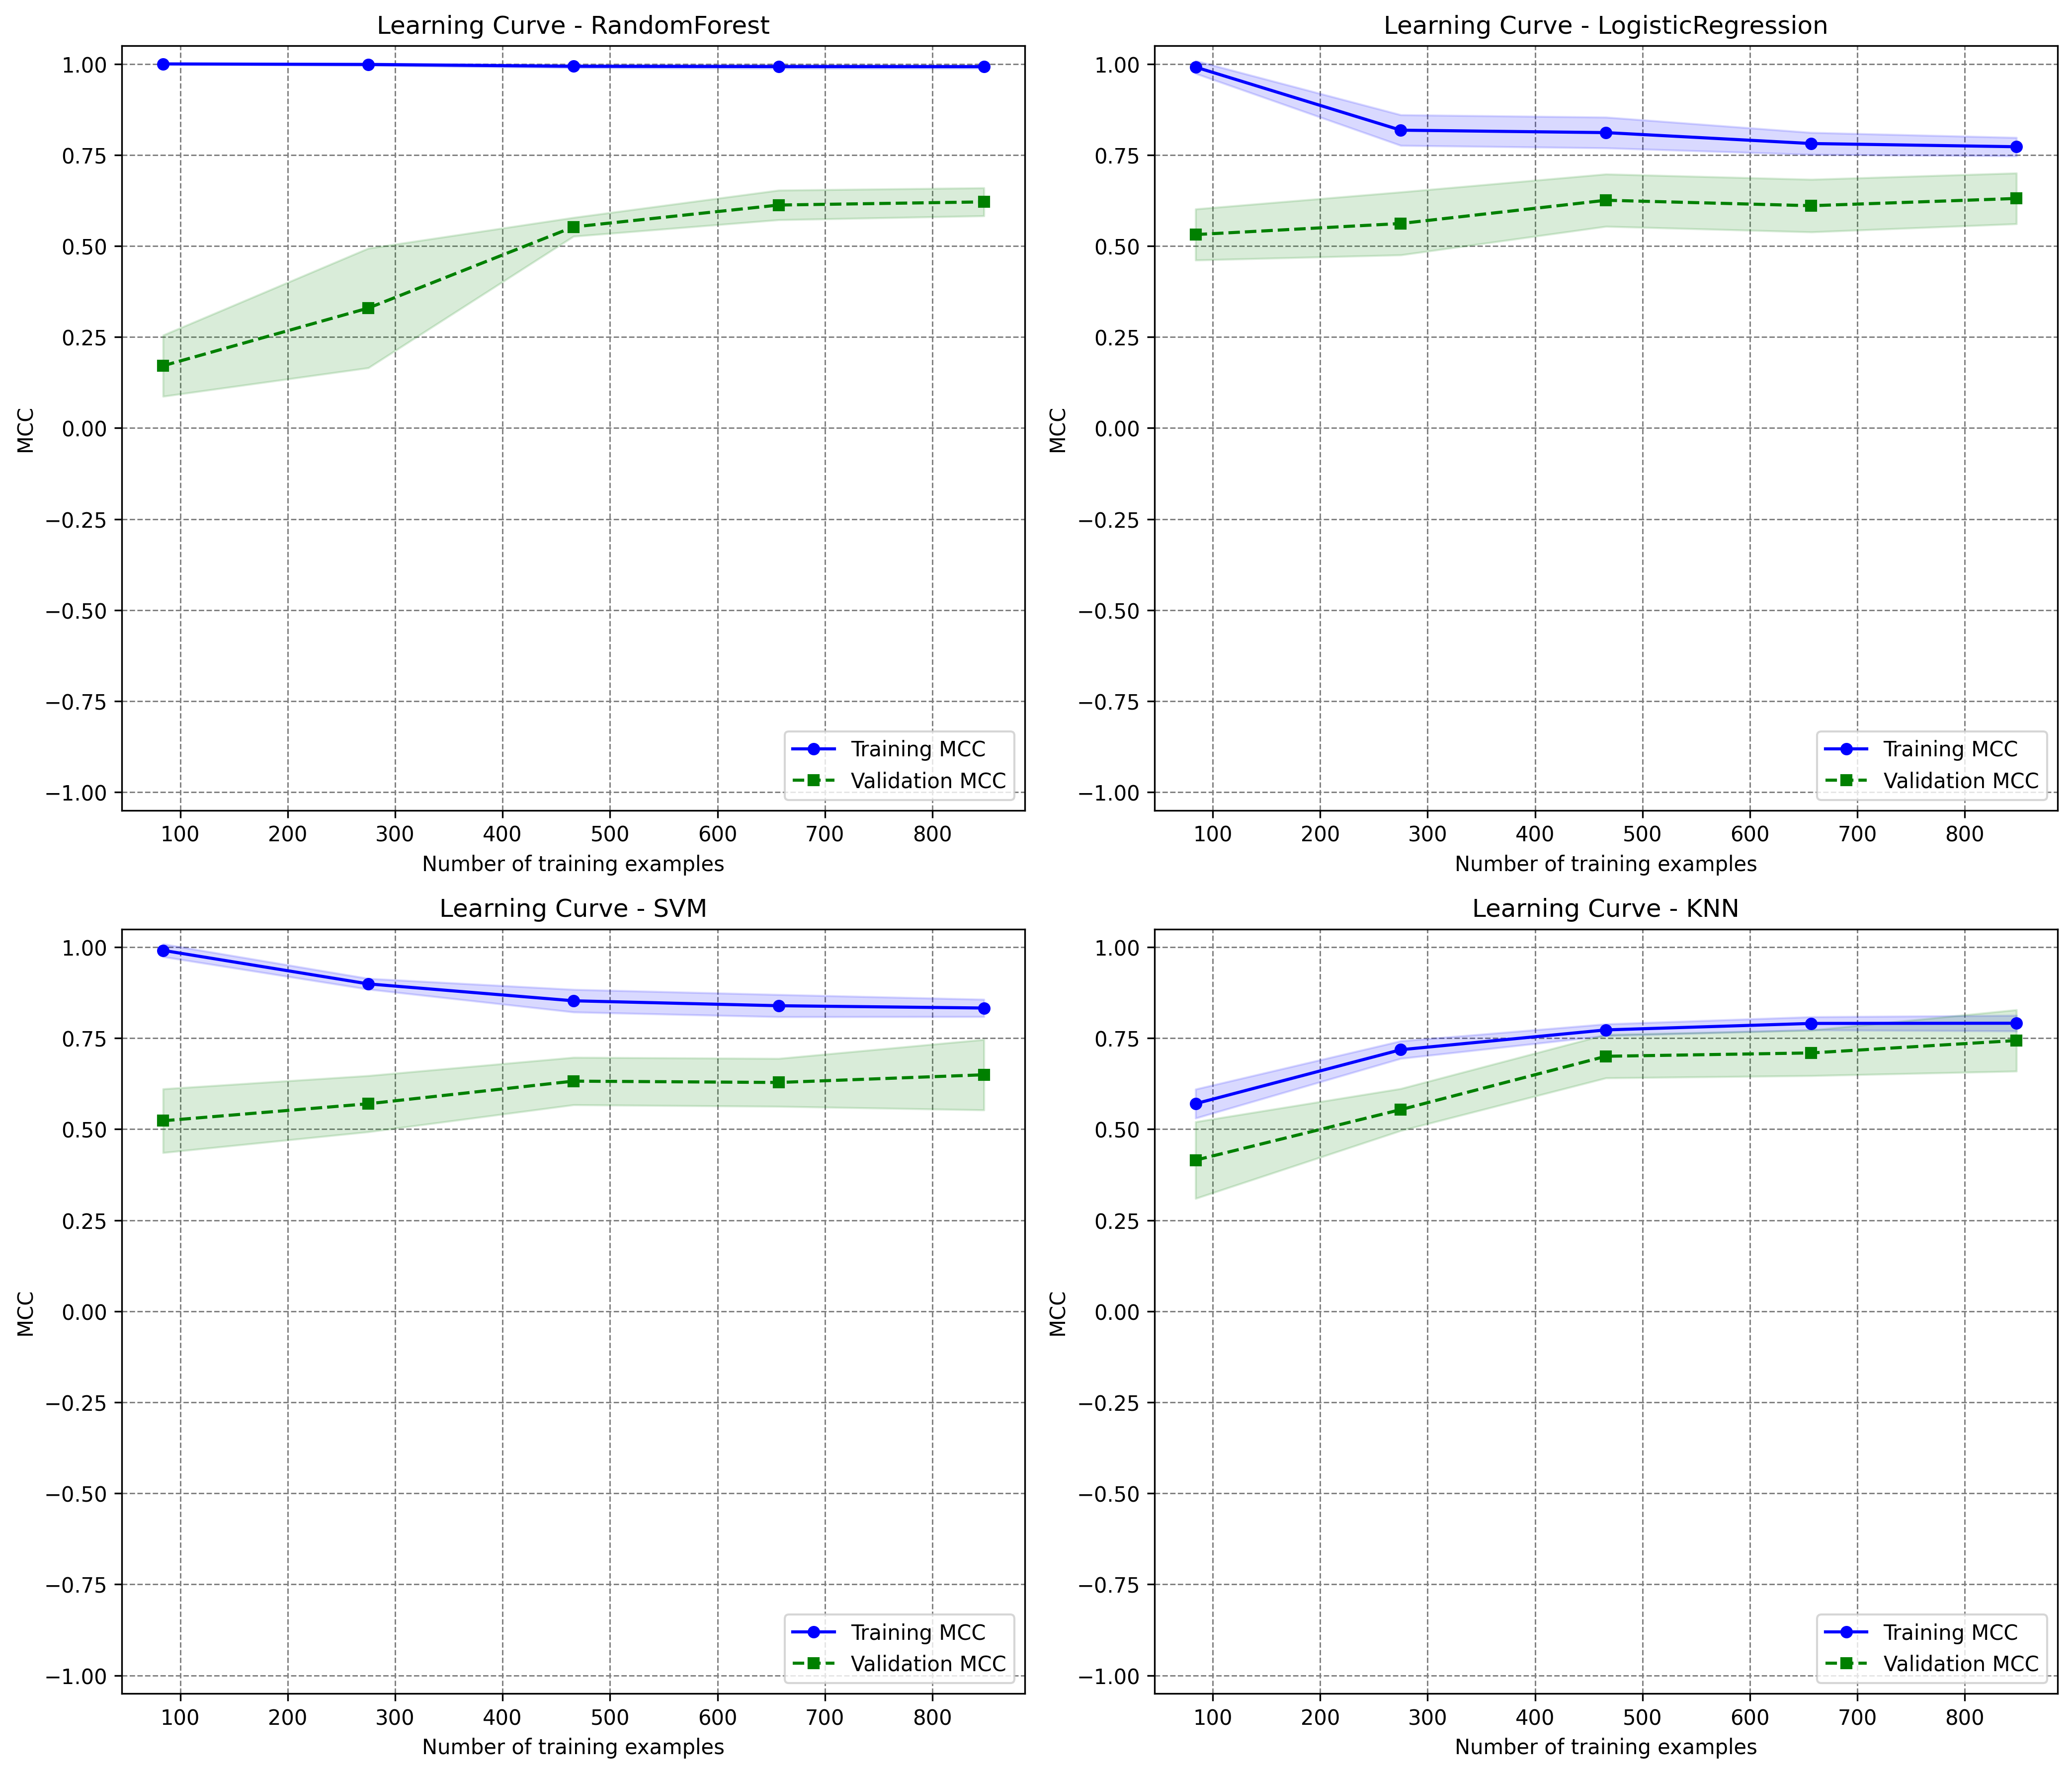
\includegraphics[width=\textwidth]{images/2x2_learning_curves_import_test_type.png}
		\caption{Learning Curves - Import Test Type}
		\label{fig:import_test_learning_curves}
	\end{subfigure}
	
	\caption{Learning Curves for Protein Sequence-Based Embeddings}
	\label{fig:sequence_learning_curves_type}
\end{figure}

\subsubsection{Learning Curves for Protein Fold-Based Embeddings}
FOLD
\begin{figure}[H]
	\centering
	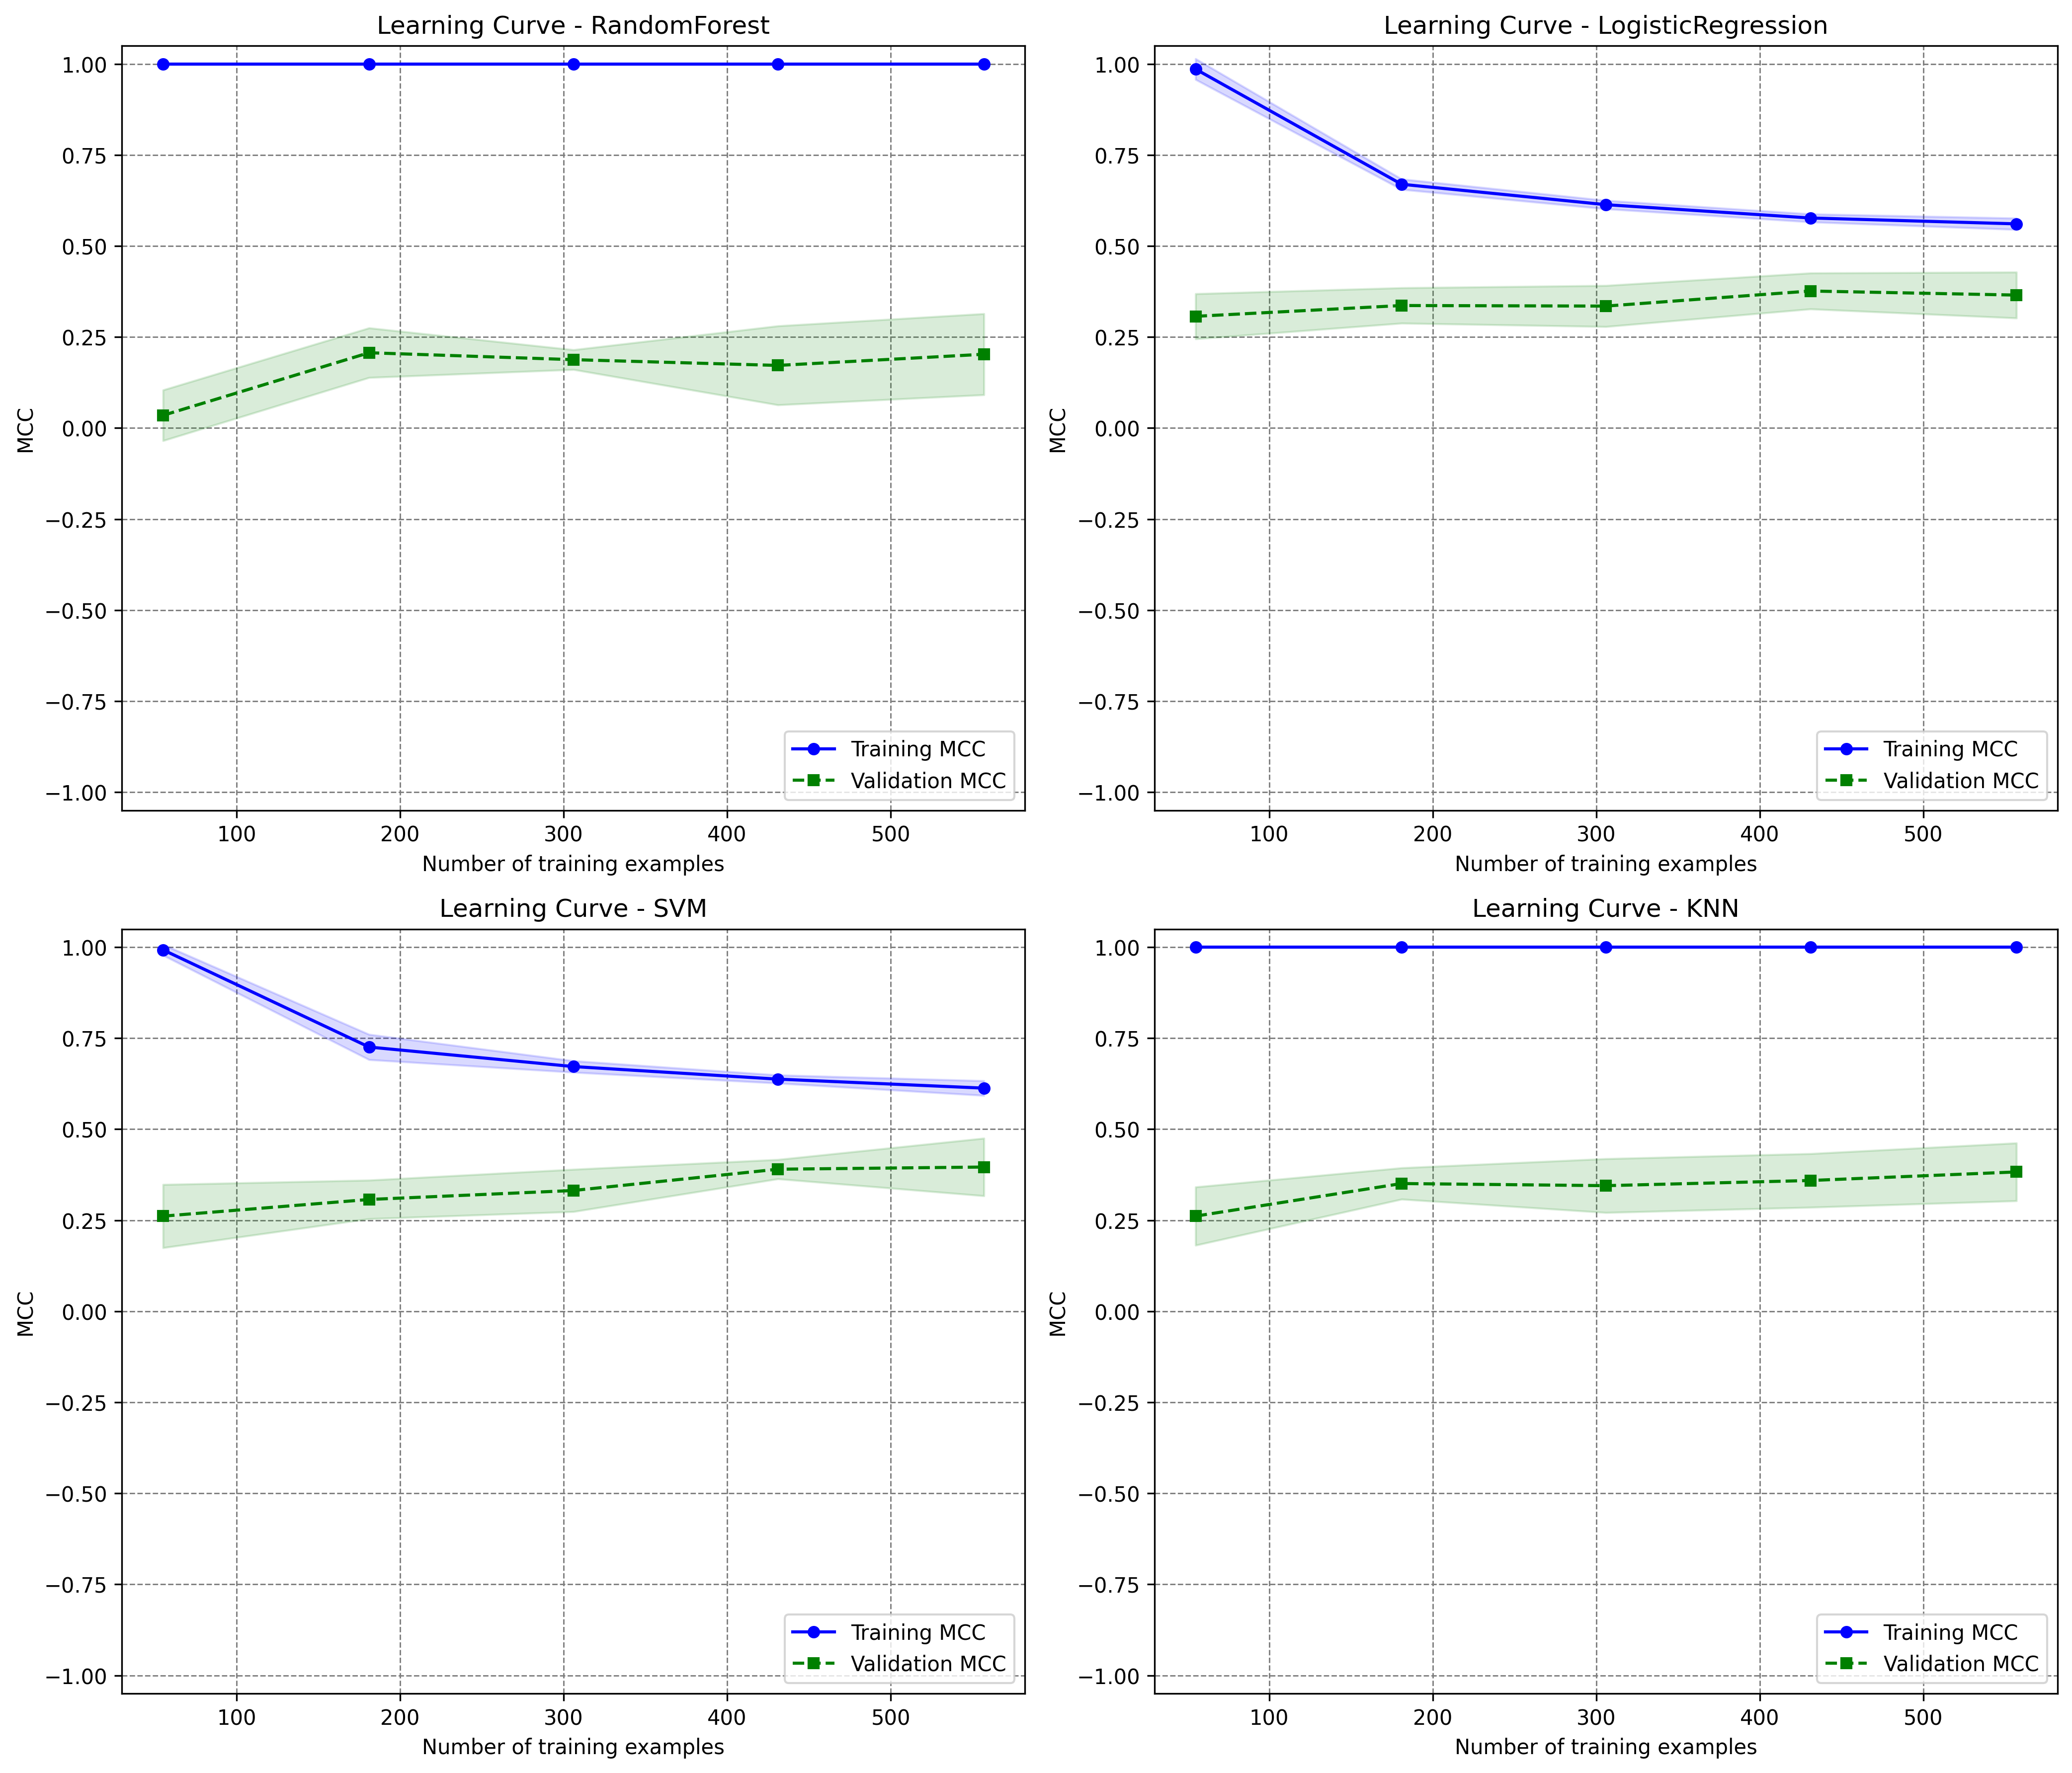
\includegraphics[width=0.7\textwidth]{images/2x2_learning_curves_folds_test_split.png}
	\caption{MCC Bar Plot for Protein Fold-Based Embeddings}
	\label{fig:learningcurve_fold_type}
\end{figure}

\subsection{Performance Evaluation}
After comparing different methods for handling test sets, a hierarchical predictor was built to mitigate data imbalance. The logic behind this hierarchical predictor was to differentiate exotoxin classes among categories with similar counts. Additionally, the models presented in the bar graph were analyzed in terms of their performance using the Matthews Correlation Coefficient (MCC).

\subsubsection{MCC Bar Plots for Protein Sequence-Based Embeddings}
\begin{figure}[H]
	\centering
	\begin{subfigure}{0.49\textwidth}
		\centering
		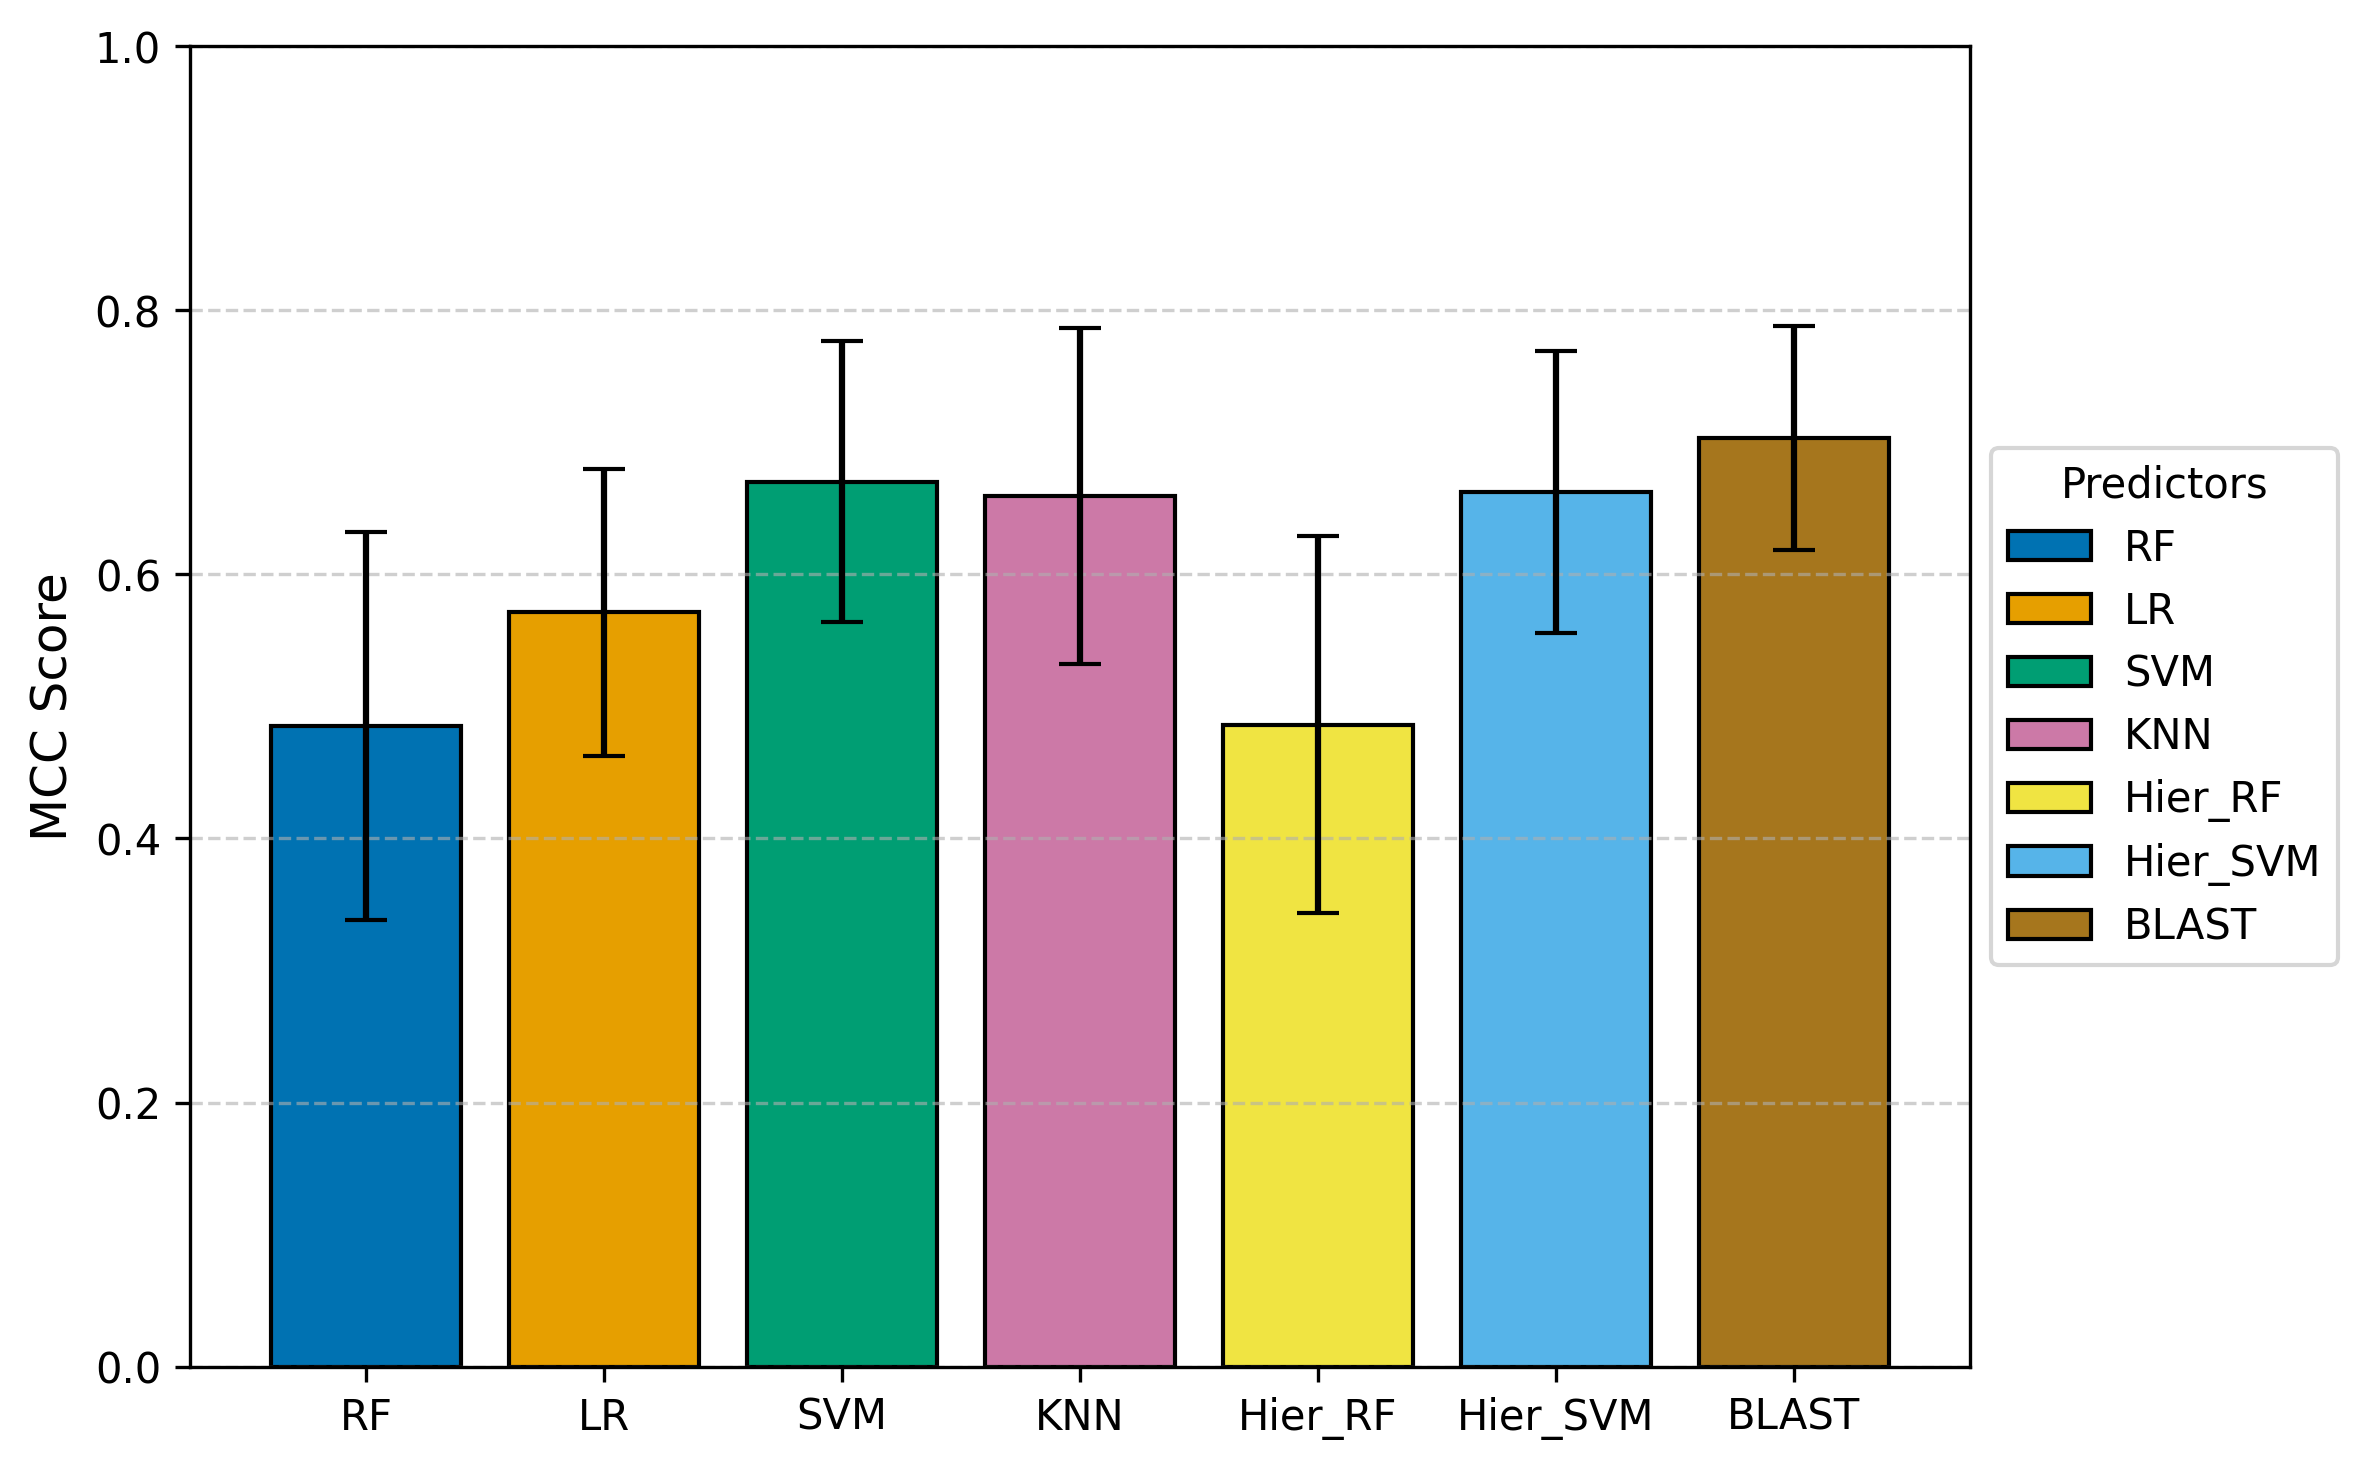
\includegraphics[width=\linewidth]{images/comparison_graph_with_error_bars_test_type_split.png}
		\caption{}
		\label{mccgraph1}
	\end{subfigure}
	\hfill
	\begin{subfigure}{0.49\textwidth}
		\centering
		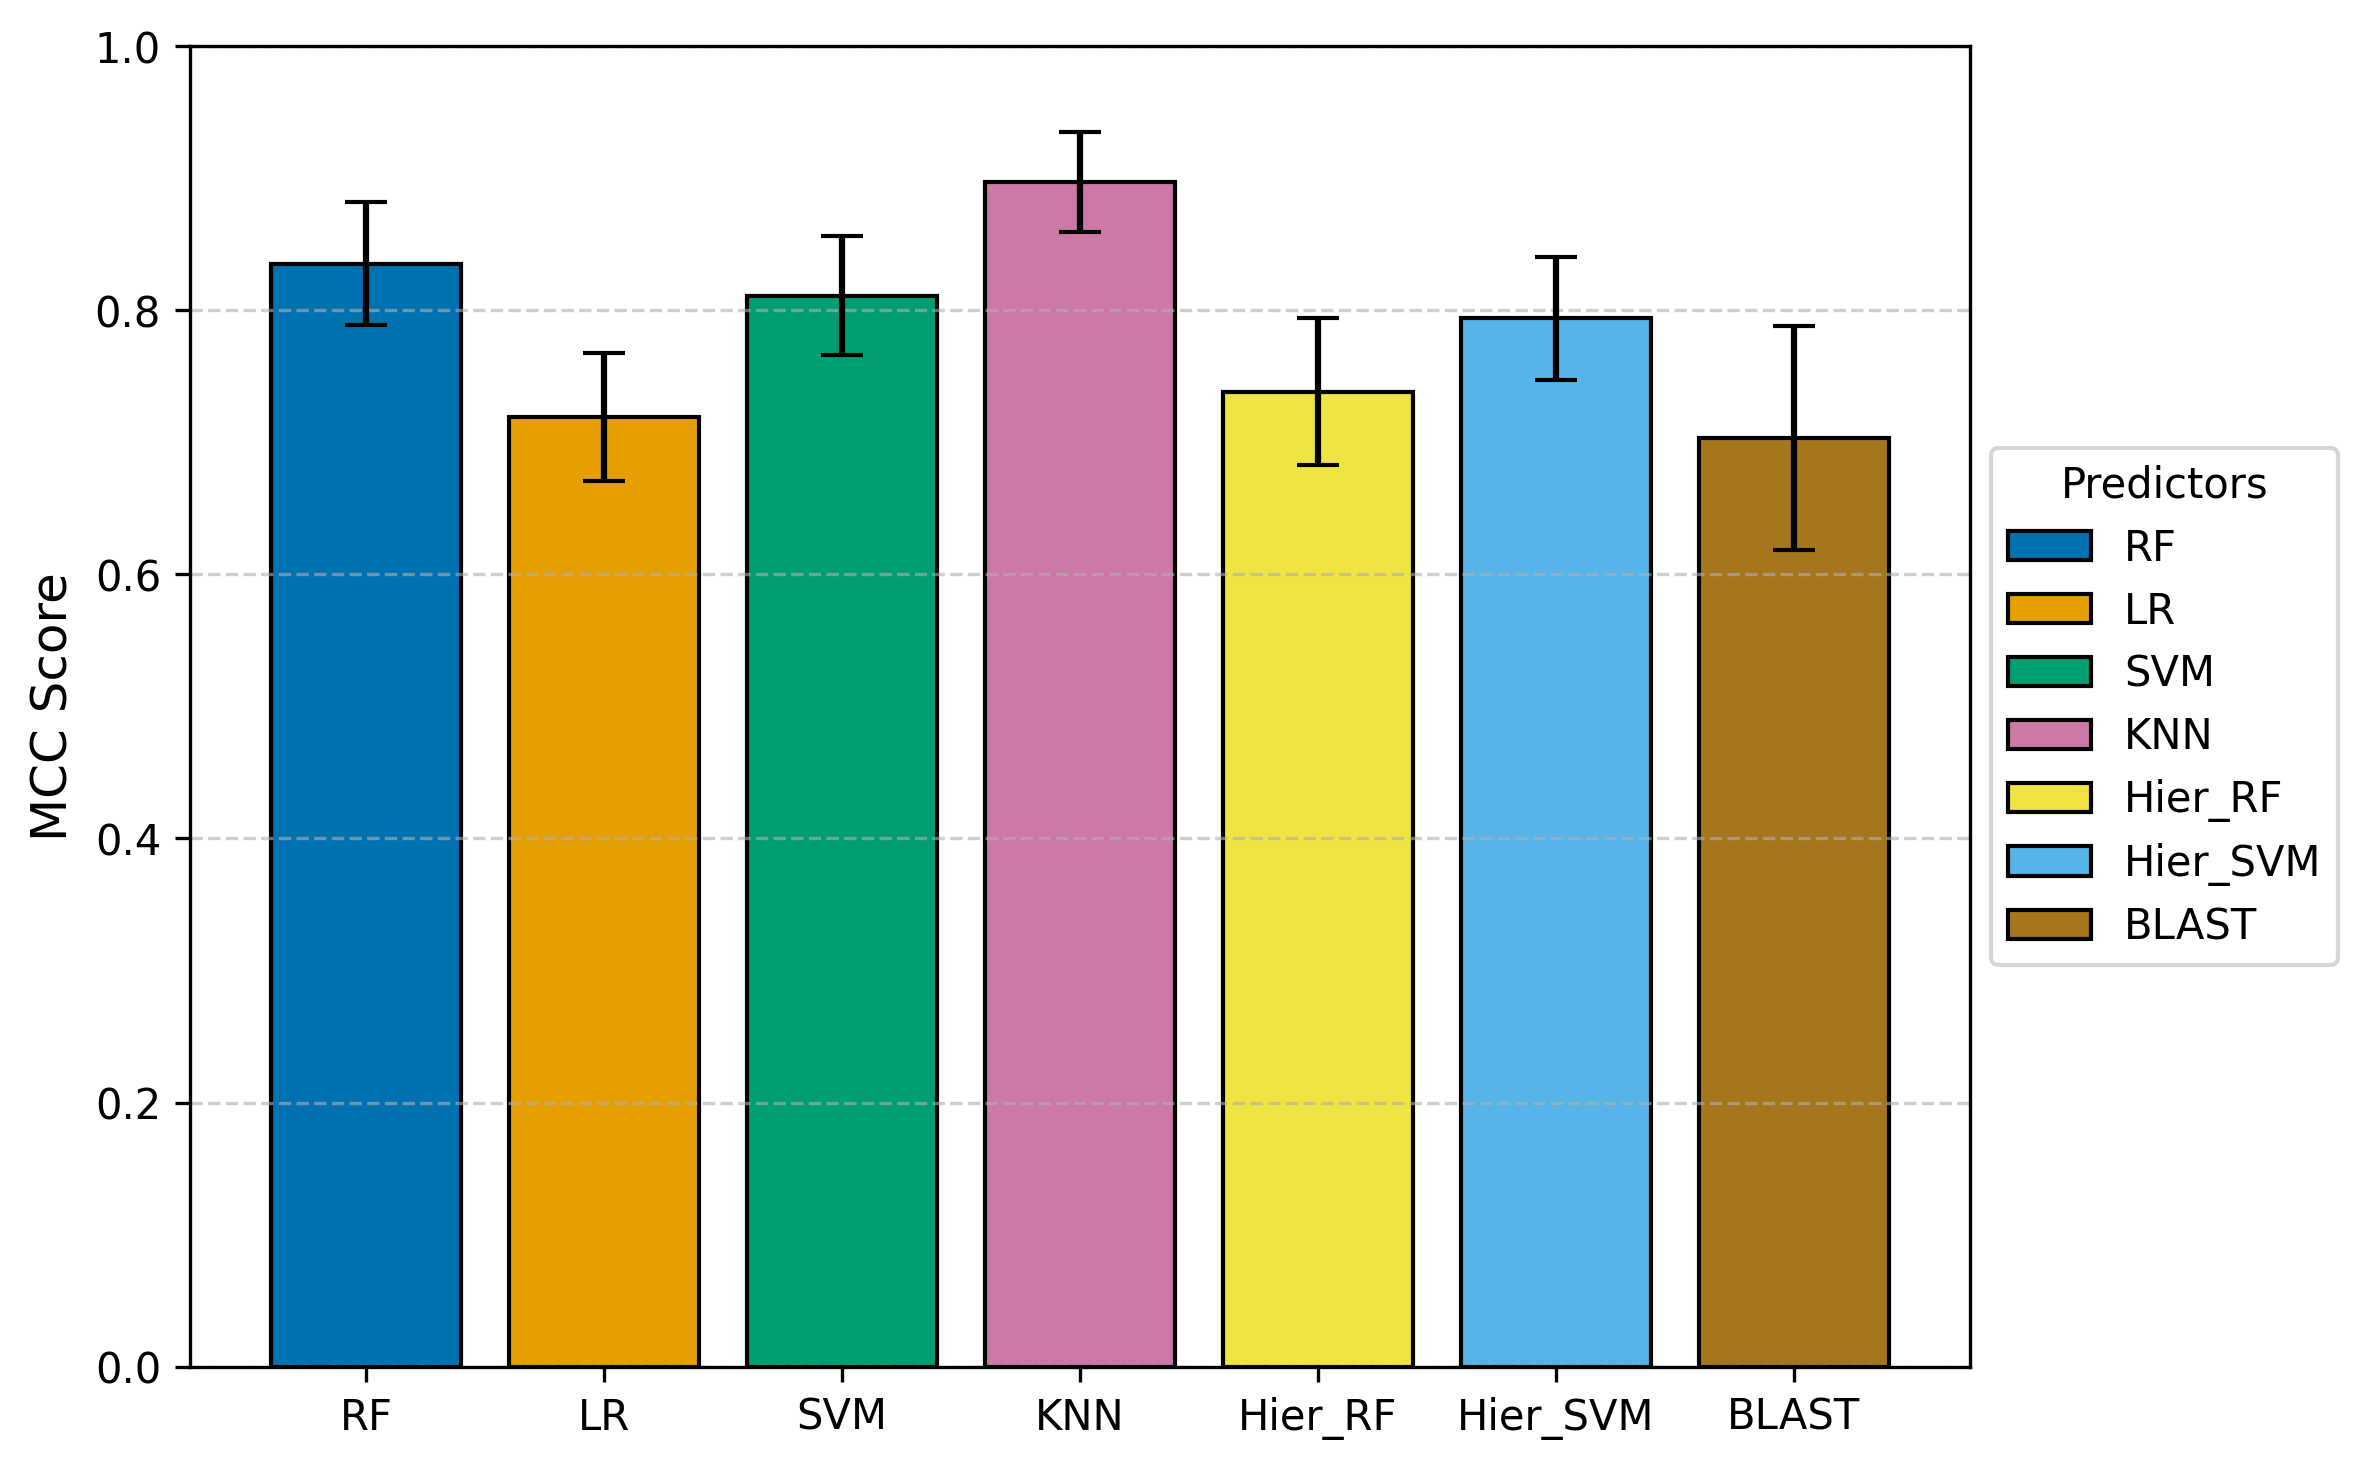
\includegraphics[width=\linewidth]{images/comparison_graph_with_error_bars_import_test_type.png}
		\caption{}
		\label{mccgraph2}
	\end{subfigure}
	\caption{MCC Bar Plots for Protein Sequence-Based Embeddings. The x-axis represents different classification models: Random Forest (RF, blue), Logistic Regression (LR, orange), Support Vector Machine (SVM, green), K-Nearest Neighbors (KNN, pink), Hierarchical Random Forest (Hier\_RF, yellow), Hierarchical Support Vector Machine (Hier\_SVM, light blue), and BLAST predictor (brown). The y-axis indicates the Matthews Correlation Coefficient (MCC) scores, with higher values reflecting better classification performance. Error bars represent the standard deviation across cross-validation folds. (a) MCC Plot 1 corresponds to the first approach, where the dataset was split into 80\% training and 20\% test set, while (b) MCC Plot 2 represents the second approach, where the entire non-redundant dataset was used for training, and previously removed redundant data was used as the test set. Models trained using the second approach generally show higher MCC scores, demonstrating the benefit of increased training data. The hierarchical models (Hier\_RF, Hier\_SVM) exhibit improved MCC scores, highlighting their ability to mitigate class imbalance.}
	\label{fig:mcc_sequence_type}
\end{figure}

In Figure~\ref{fig:mccgraph1}, SVM (0.67) and KNN (0.68) outperform other models, while Random Forest (0.55) and BLAST (0.60) show moderate performance. Hierarchical SVM (0.62) improves over standard SVM, indicating better handling of class imbalance. Logistic Regression and Hierarchical Random Forest perform worse, with MCC values below 0.50.

In Figure~\ref{fig:mccgraph2}, SVM and KNN exceed 0.80, while Hierarchical SVM reaches ~0.78, reinforcing its robustness. Random Forest (0.75) and BLAST (0.72) improve notably, but Hierarchical Random Forest (0.65) still lags behind. The second approach results in higher MCC scores across models, showing the advantage of a larger training set. Hierarchical models consistently perform better, particularly Hierarchical SVM, which balances class distributions effectively.

\subsubsection{MCC Bar Plots for Protein Protein Fold-Based Embeddings}
\begin{figure}[H]
	\centering
	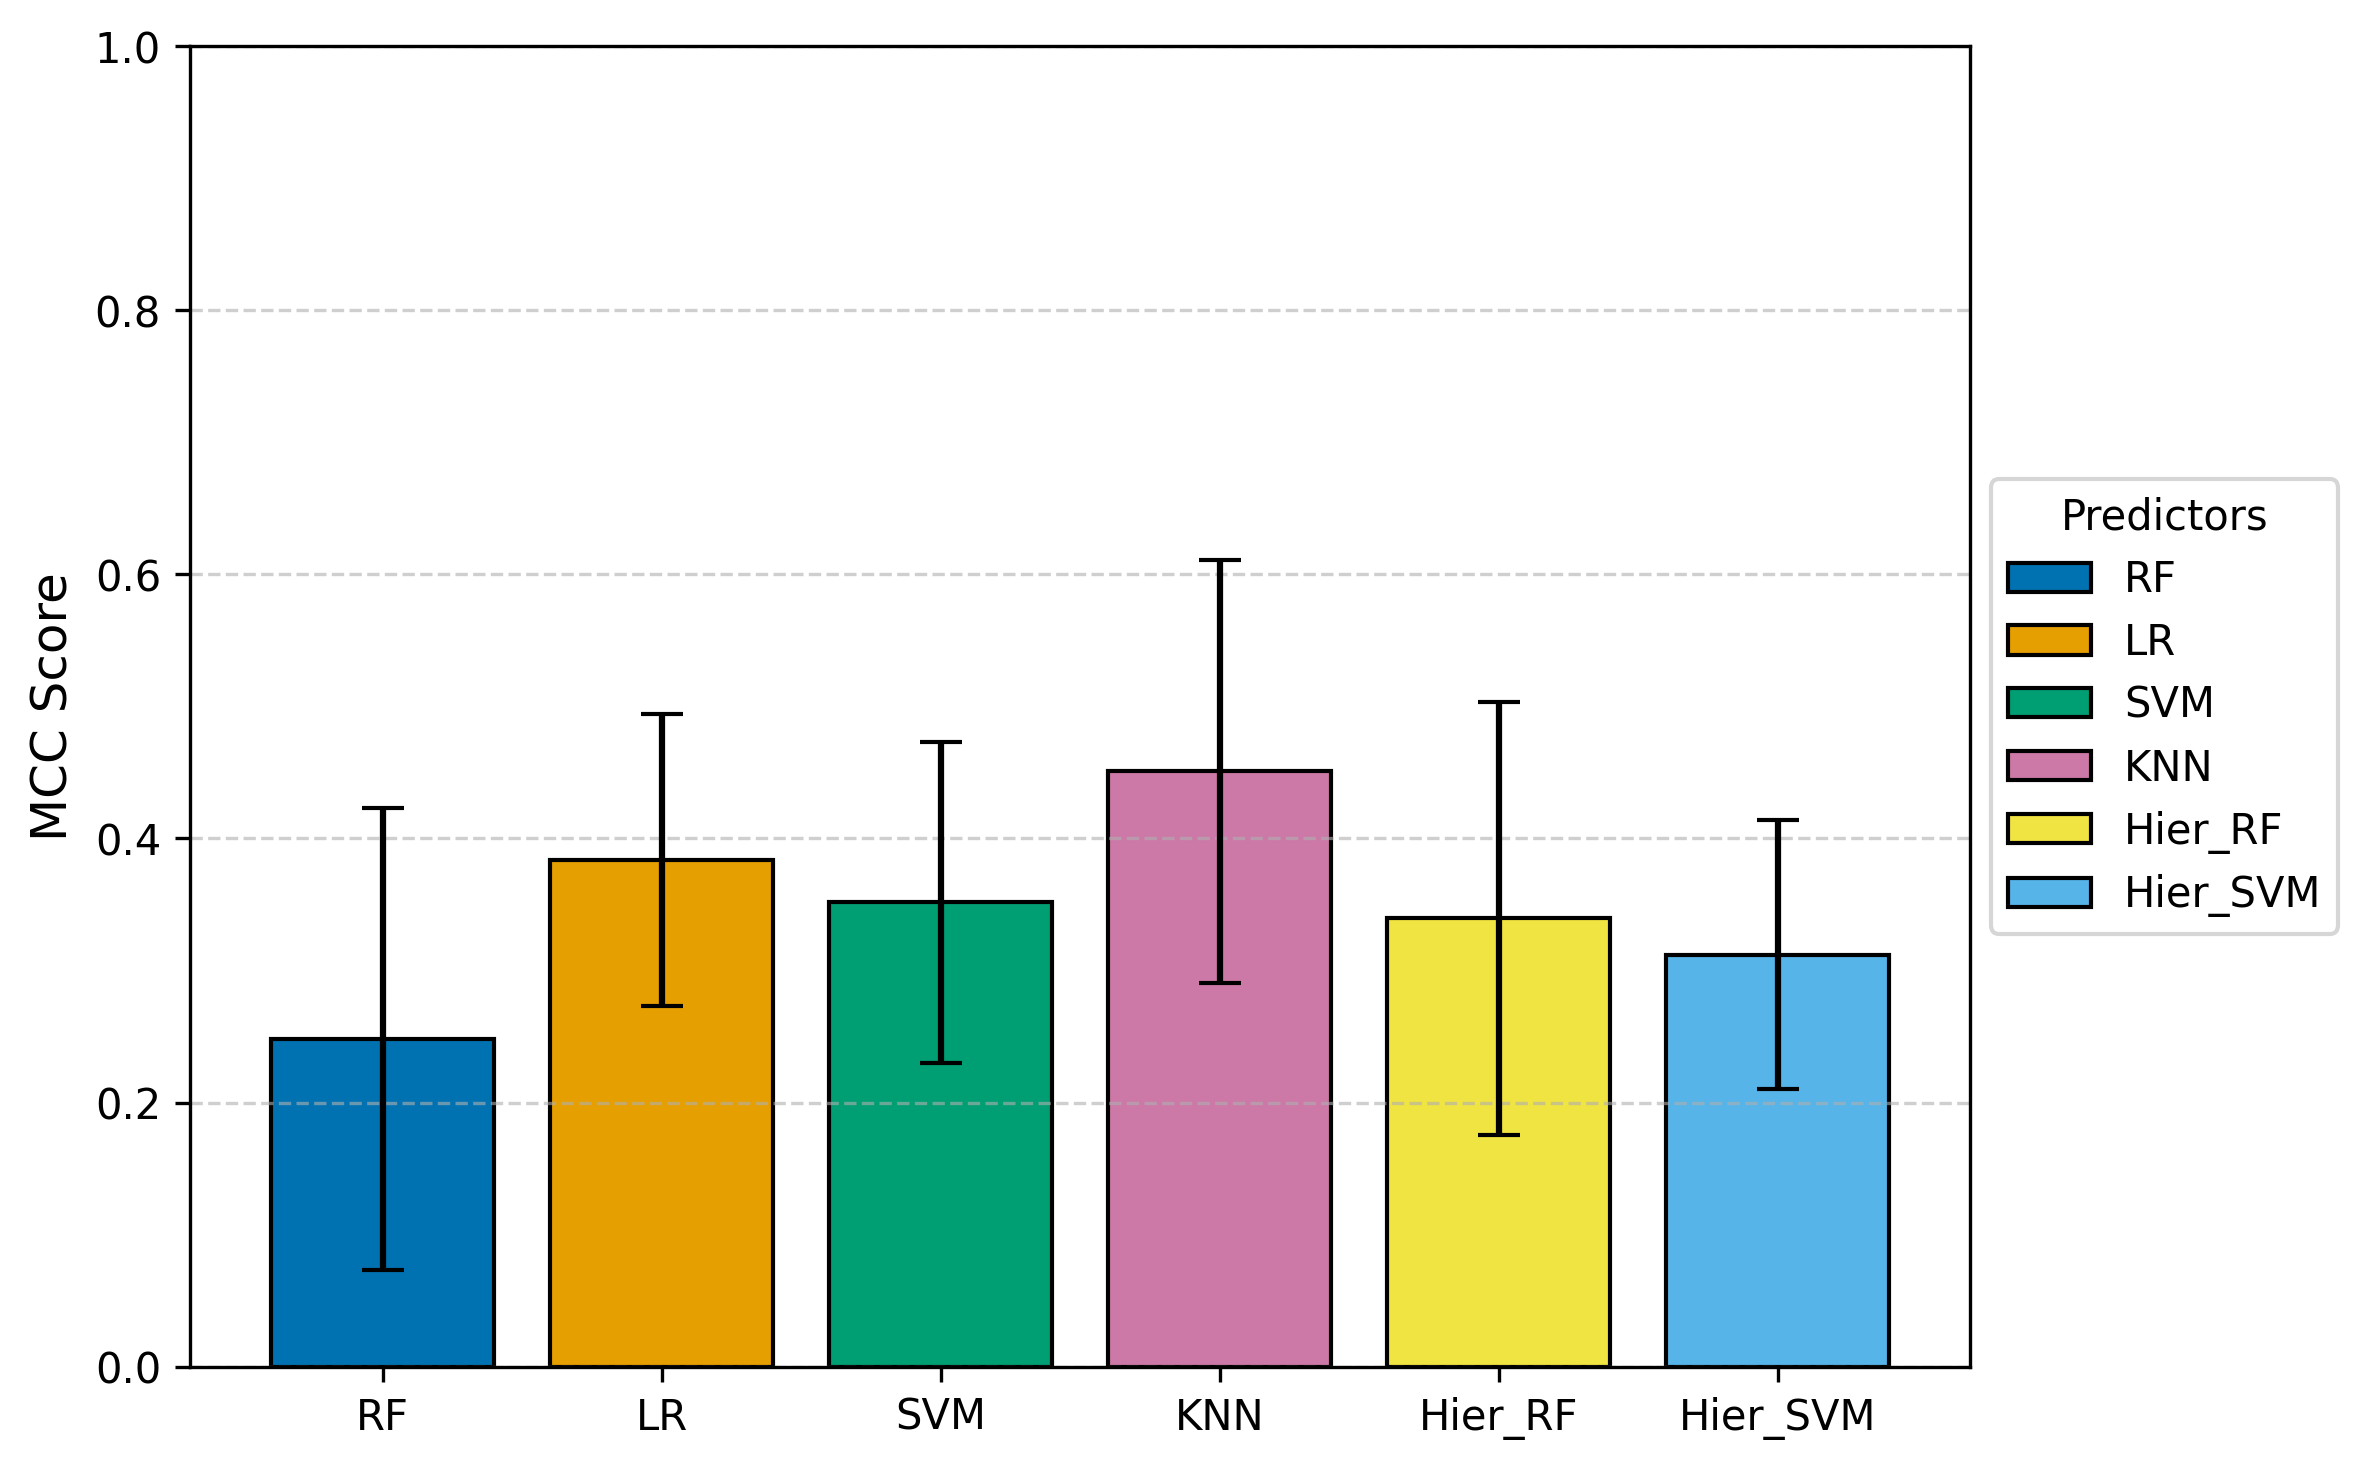
\includegraphics[width=0.7\textwidth]{images/comparison_graph_with_error_bars_folds_test_split_type.png}
	\caption{MCC Bar Plot for Protein Fold-Based Embeddings}
	\label{fig:mcc_fold_type}
\end{figure}

\subsubsection{ROC Curves for Protein Sequence-Based Embeddings}
\begin{figure}[H]
	\centering
	\begin{subfigure}{0.49\textwidth}
		\centering
		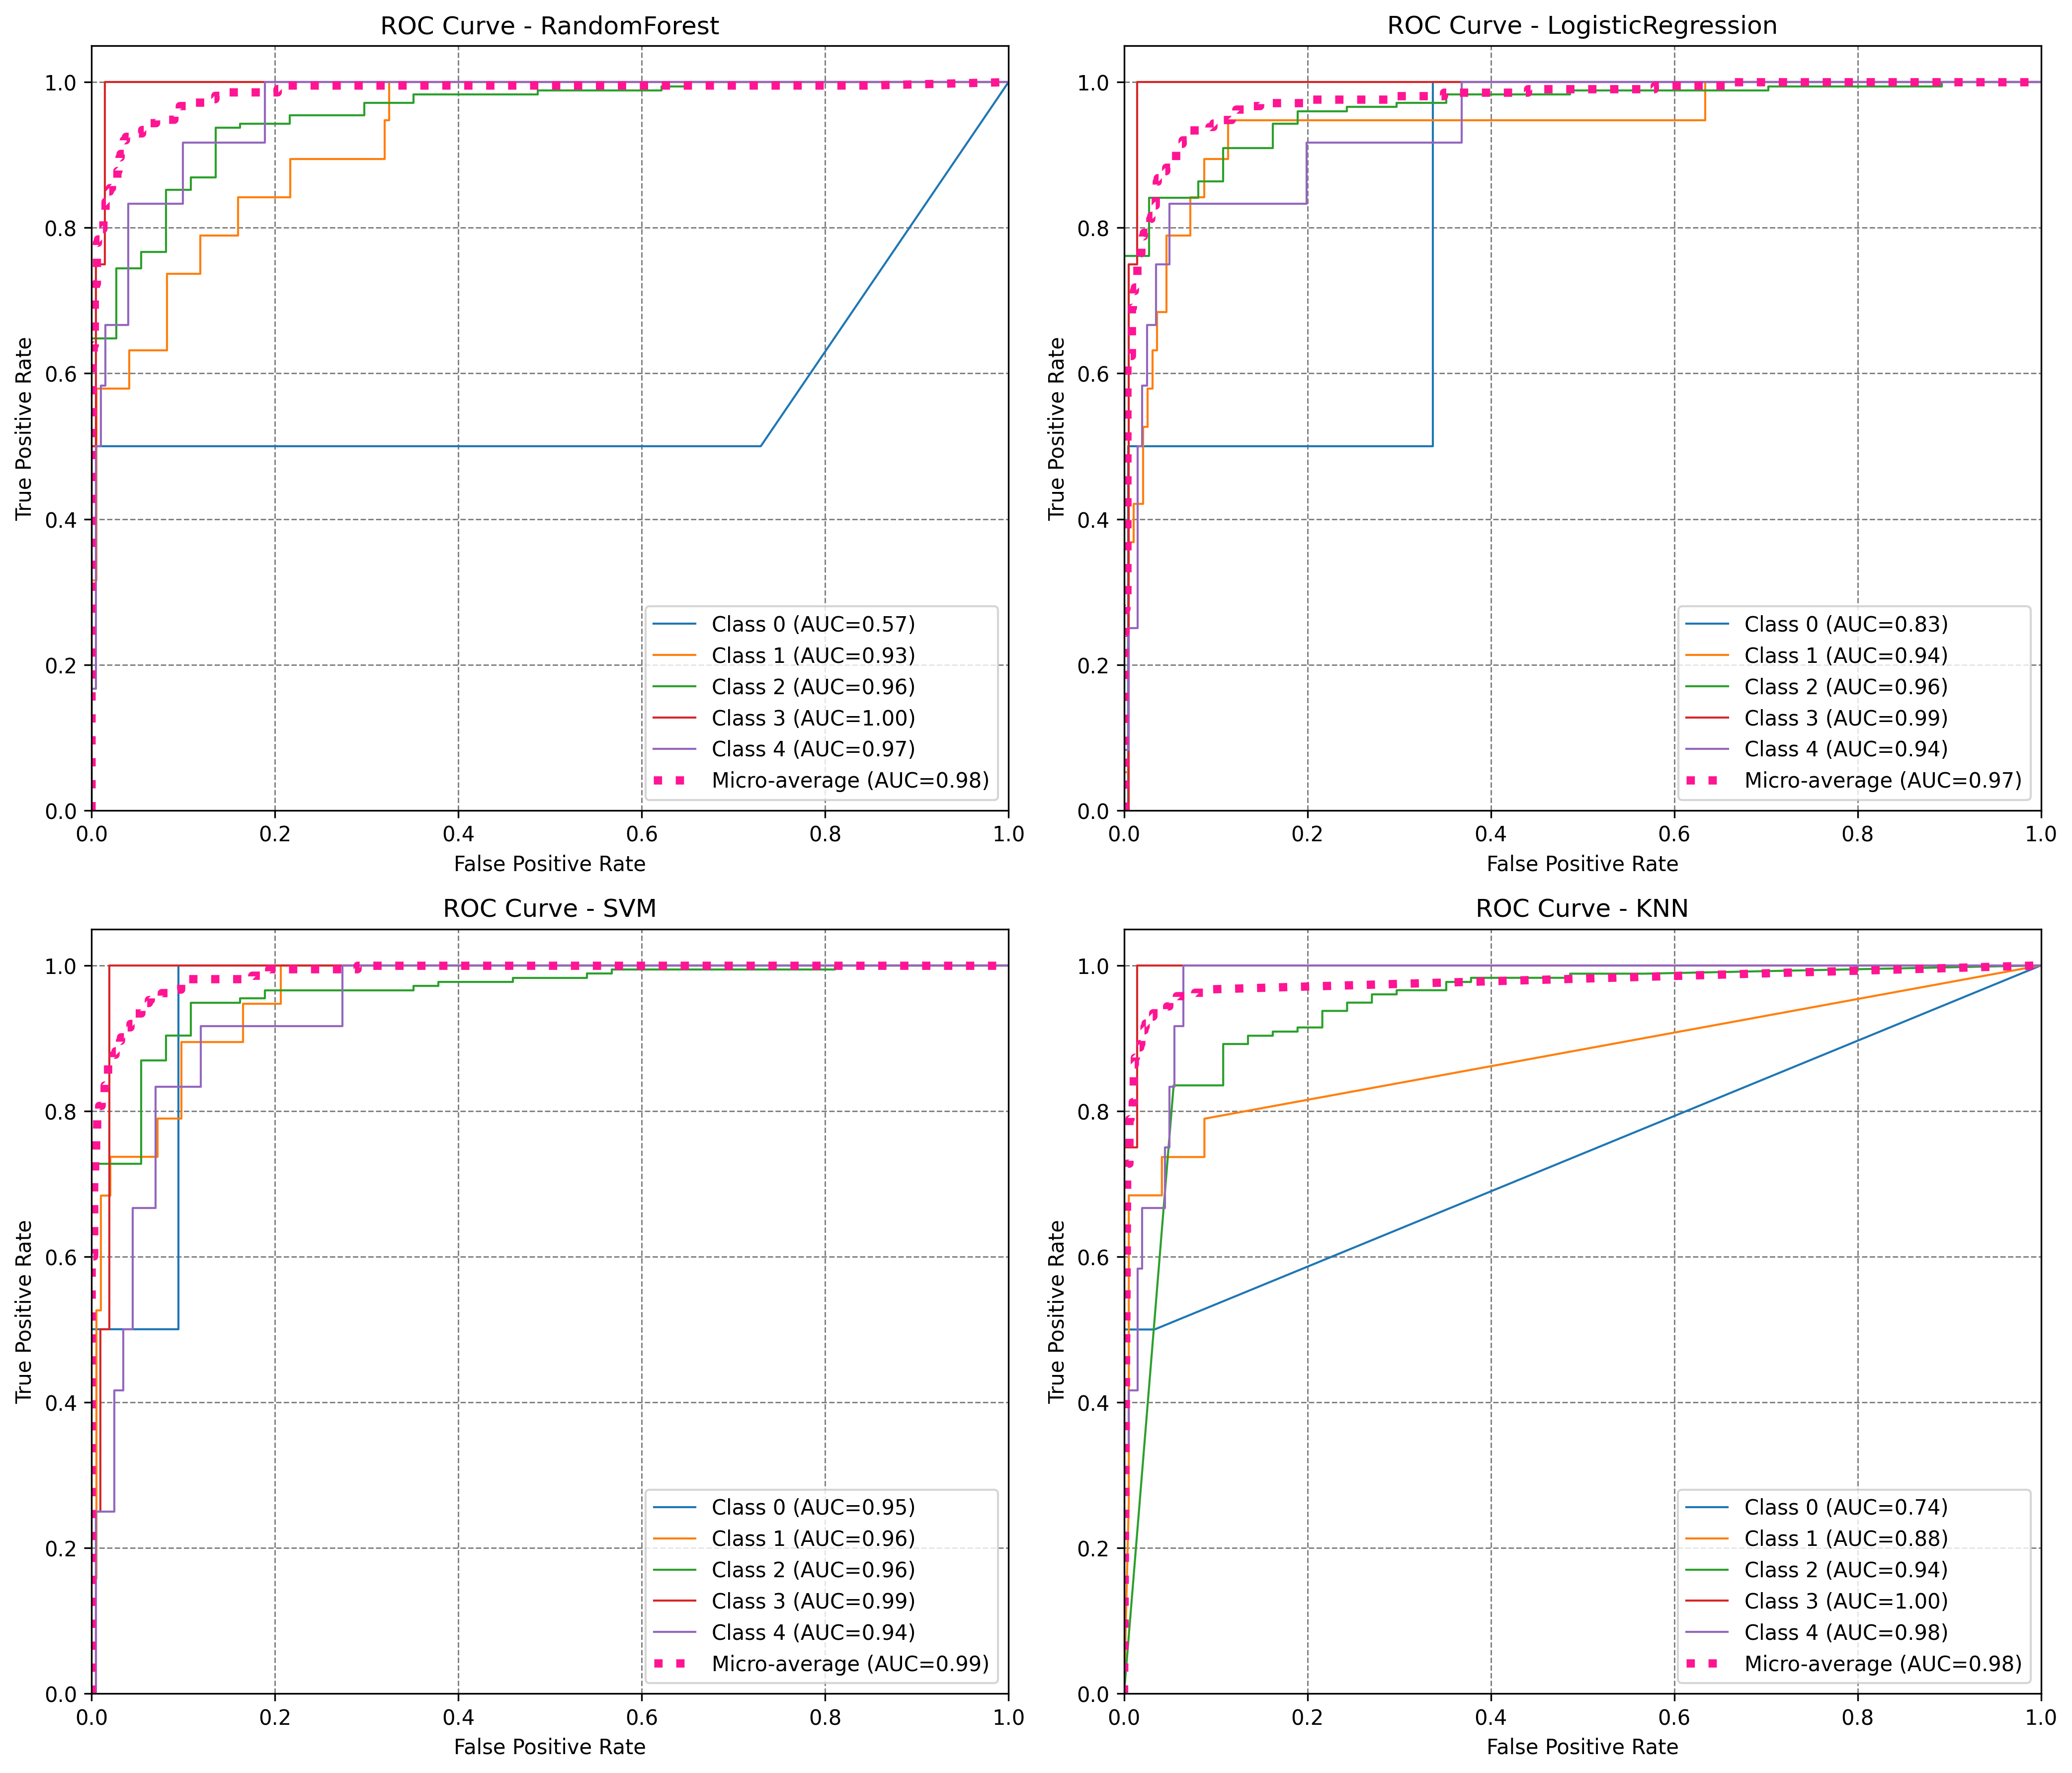
\includegraphics[width=\linewidth]{images/2x2_roc_curves_split_test_type.png}
		\caption{ROC Curve 1}
	\end{subfigure}
	\hfill
	\begin{subfigure}{0.49\textwidth}
		\centering
		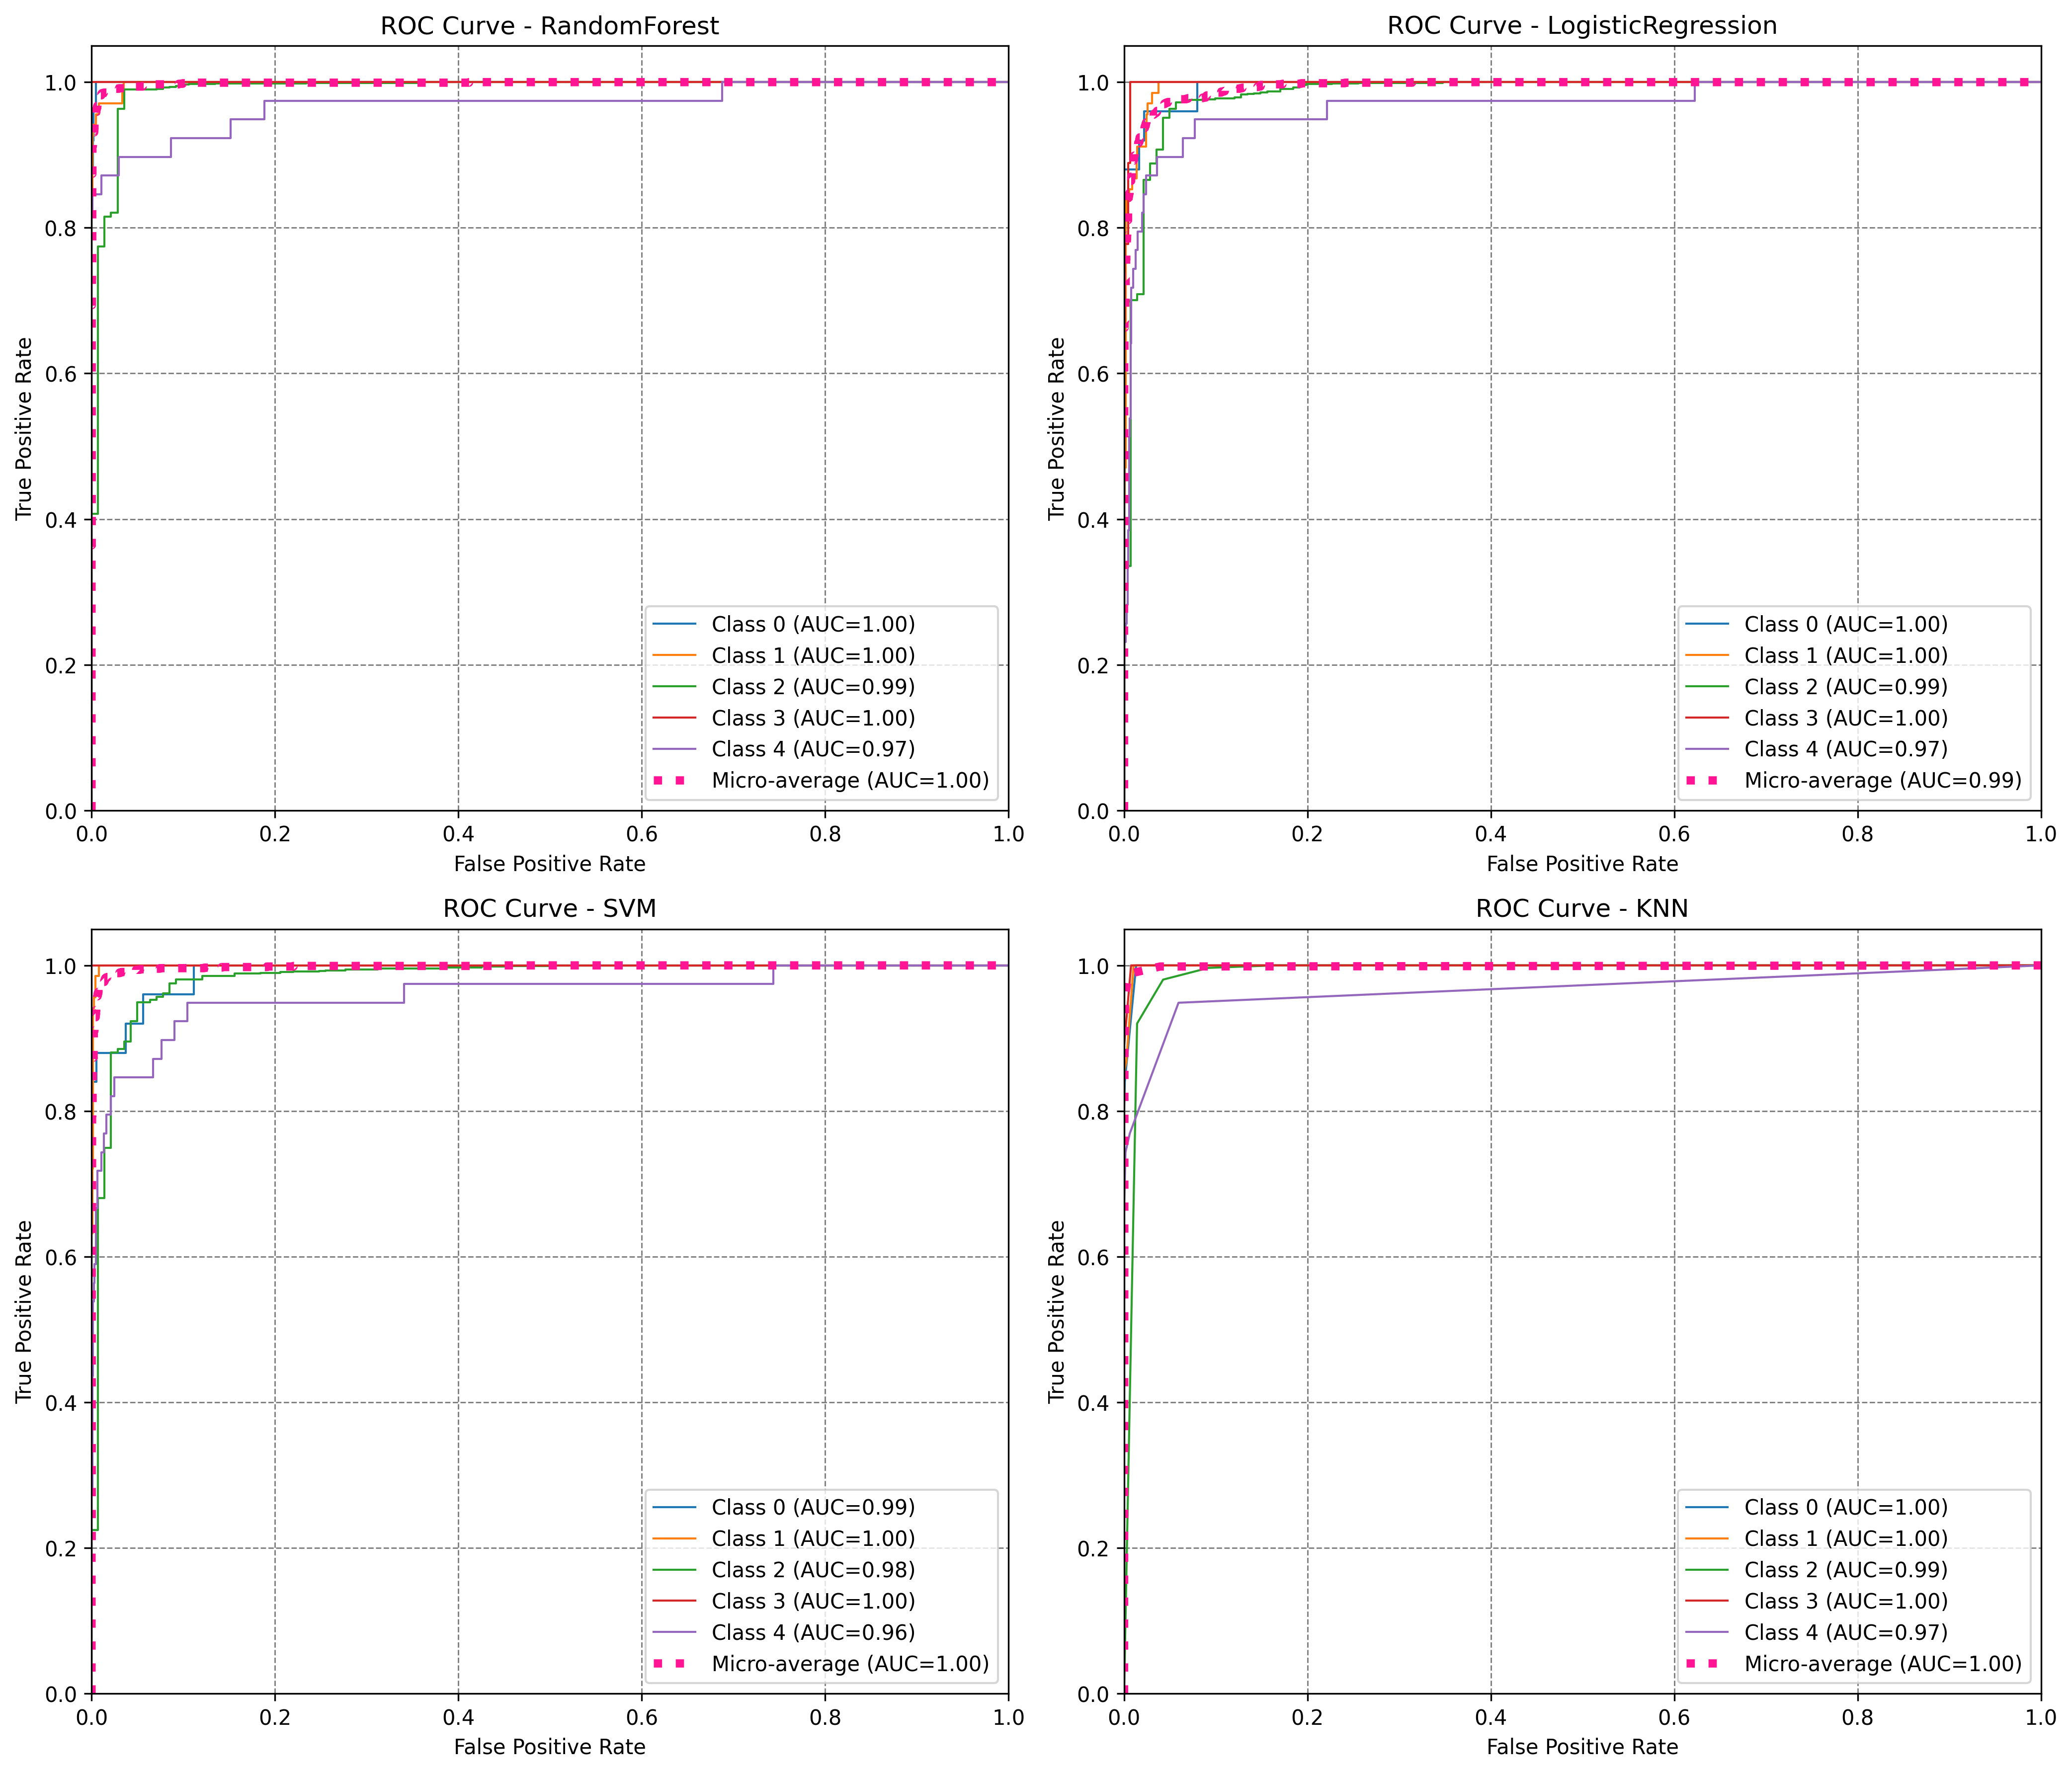
\includegraphics[width=\linewidth]{images/2x2_roc_curves_import_test_type.png}
		\caption{ROC Curve 2}
	\end{subfigure}
	\caption{ROC Curves for Protein Sequence-Based Embeddings}
	\label{fig:roc_sequence}
\end{figure}

\subsubsection{ROC Curves for Protein Protein Fold-Based Embeddings}
\begin{figure}[H]
	\centering
	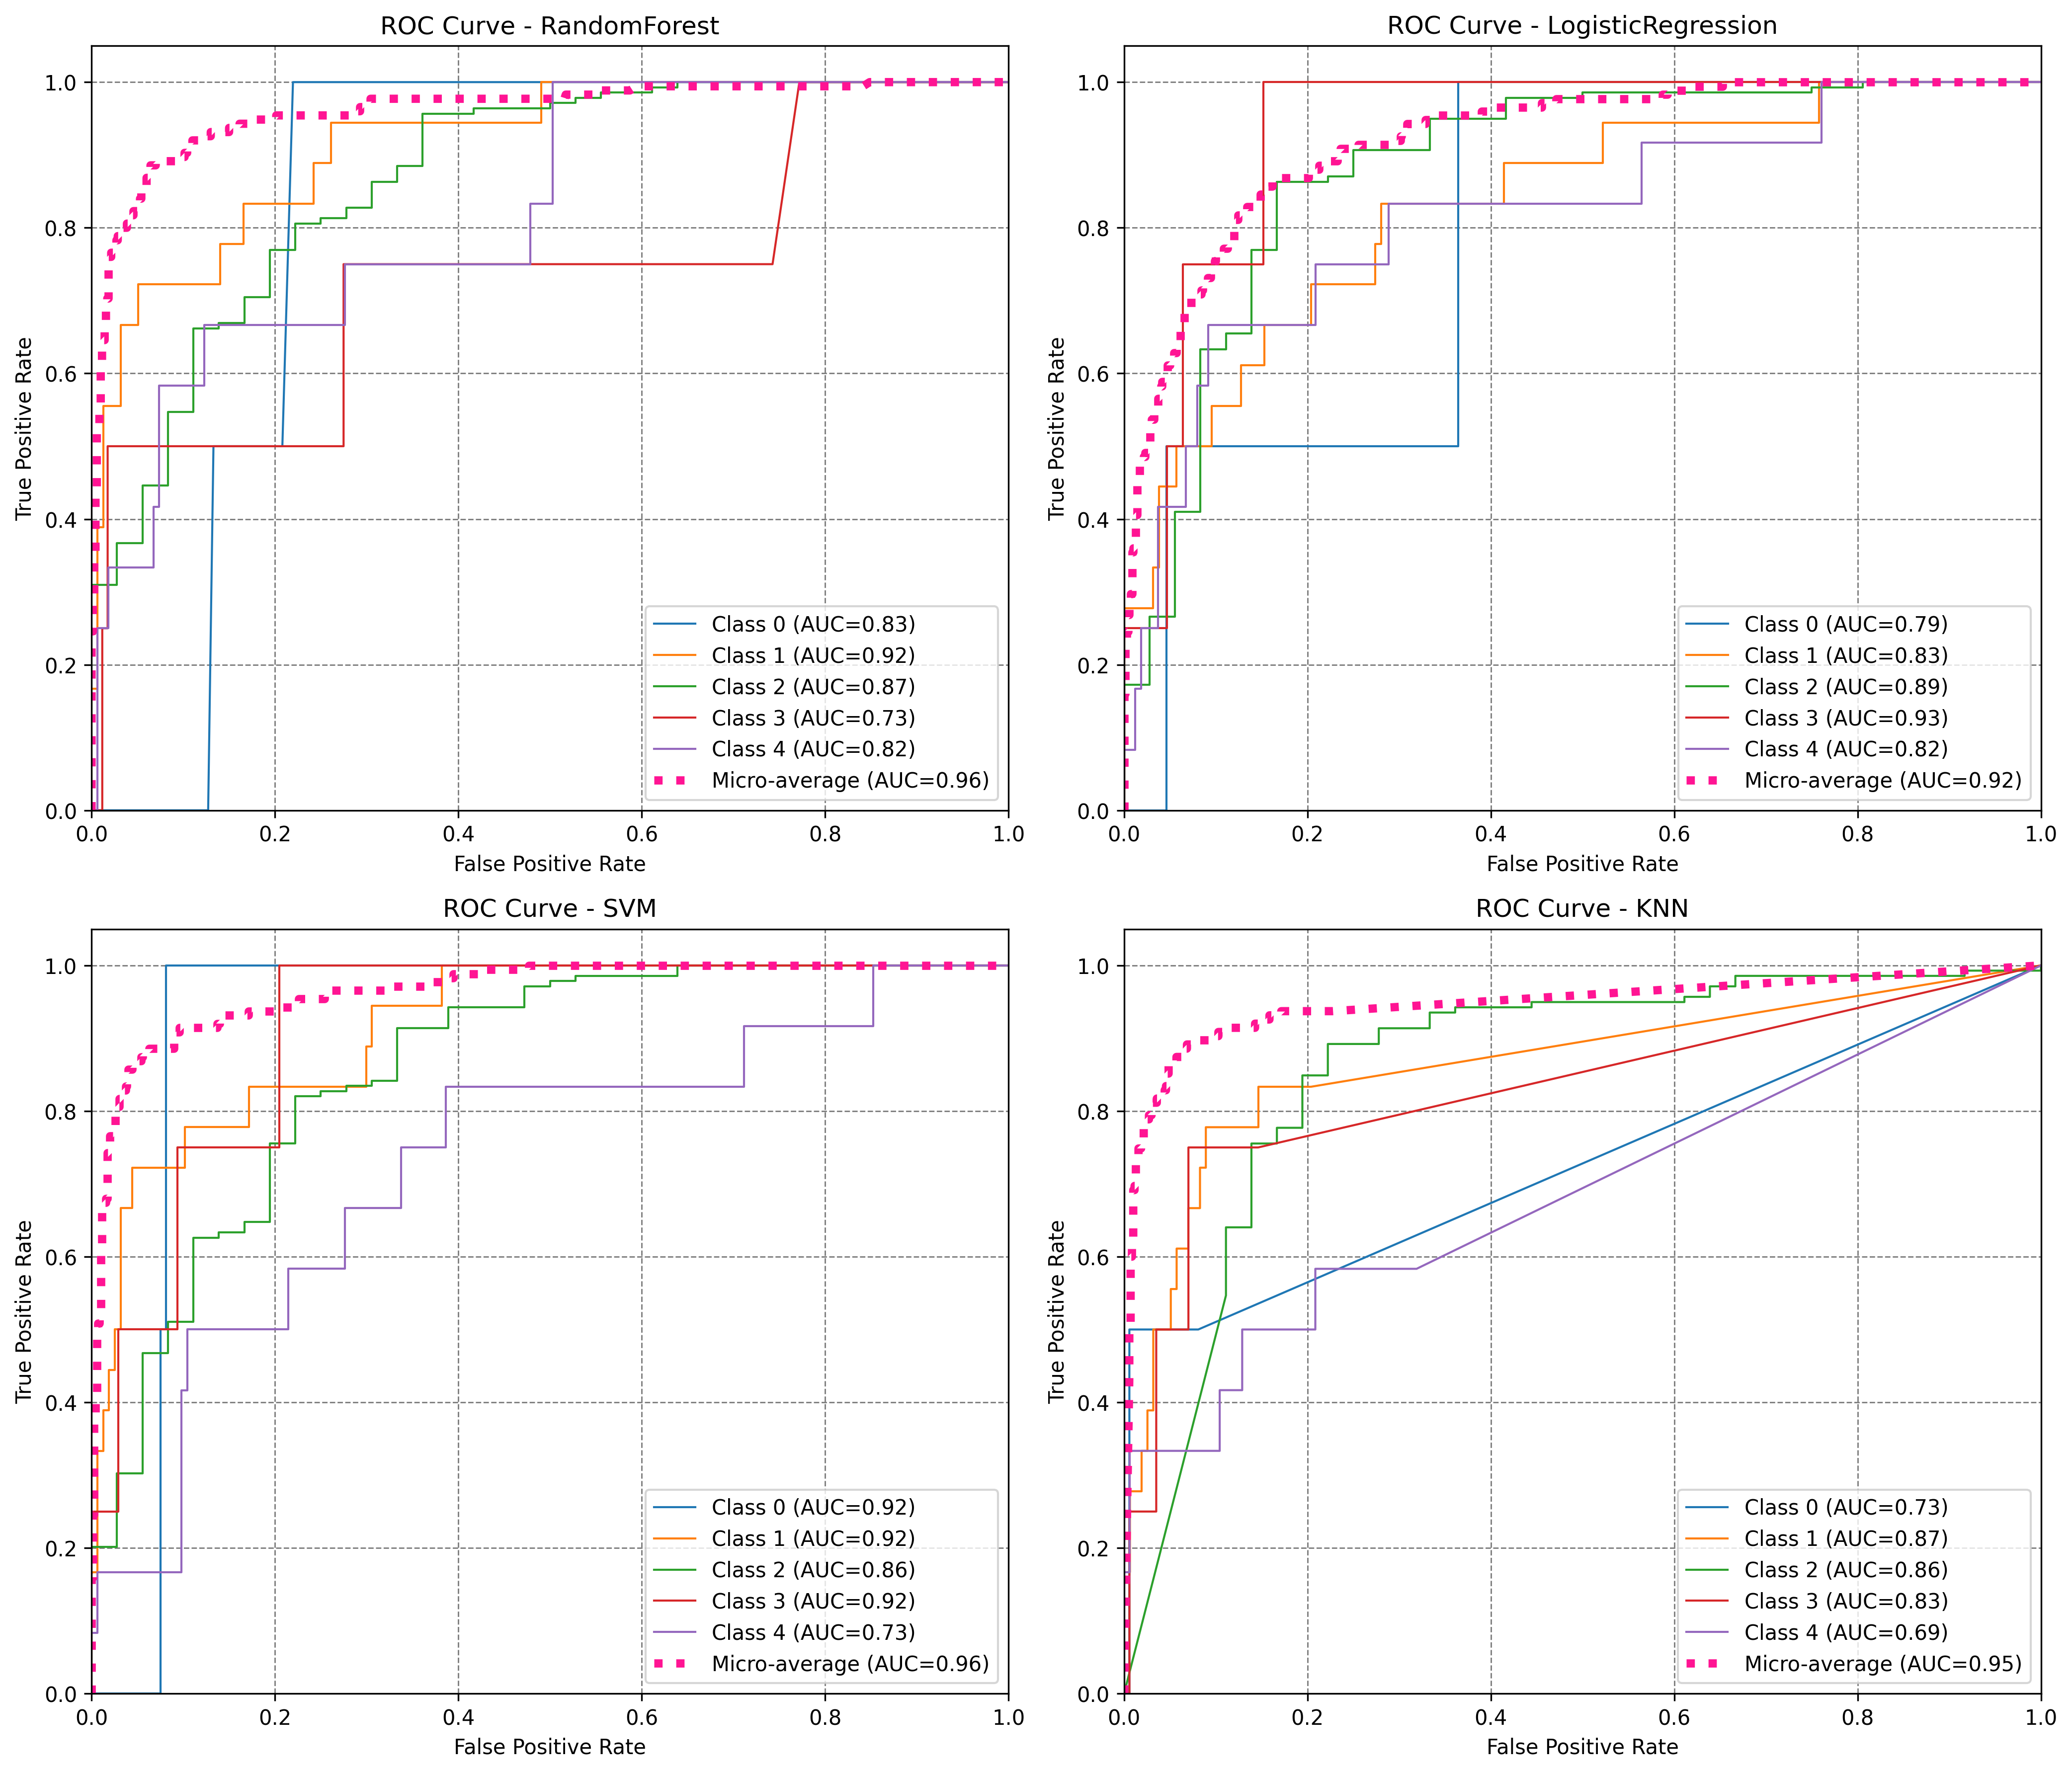
\includegraphics[width=0.7\textwidth]{images/2x2_roc_curves_folds_test_split.png}
	\caption{ROC Curve for Protein Fold-Based Embeddings}
	\label{fig:roc_fold}
\end{figure}

\subsubsection{Precision-Recall Curves for Protein Protein Sequence-Based Embeddings}
\begin{figure}[H]
	\centering
	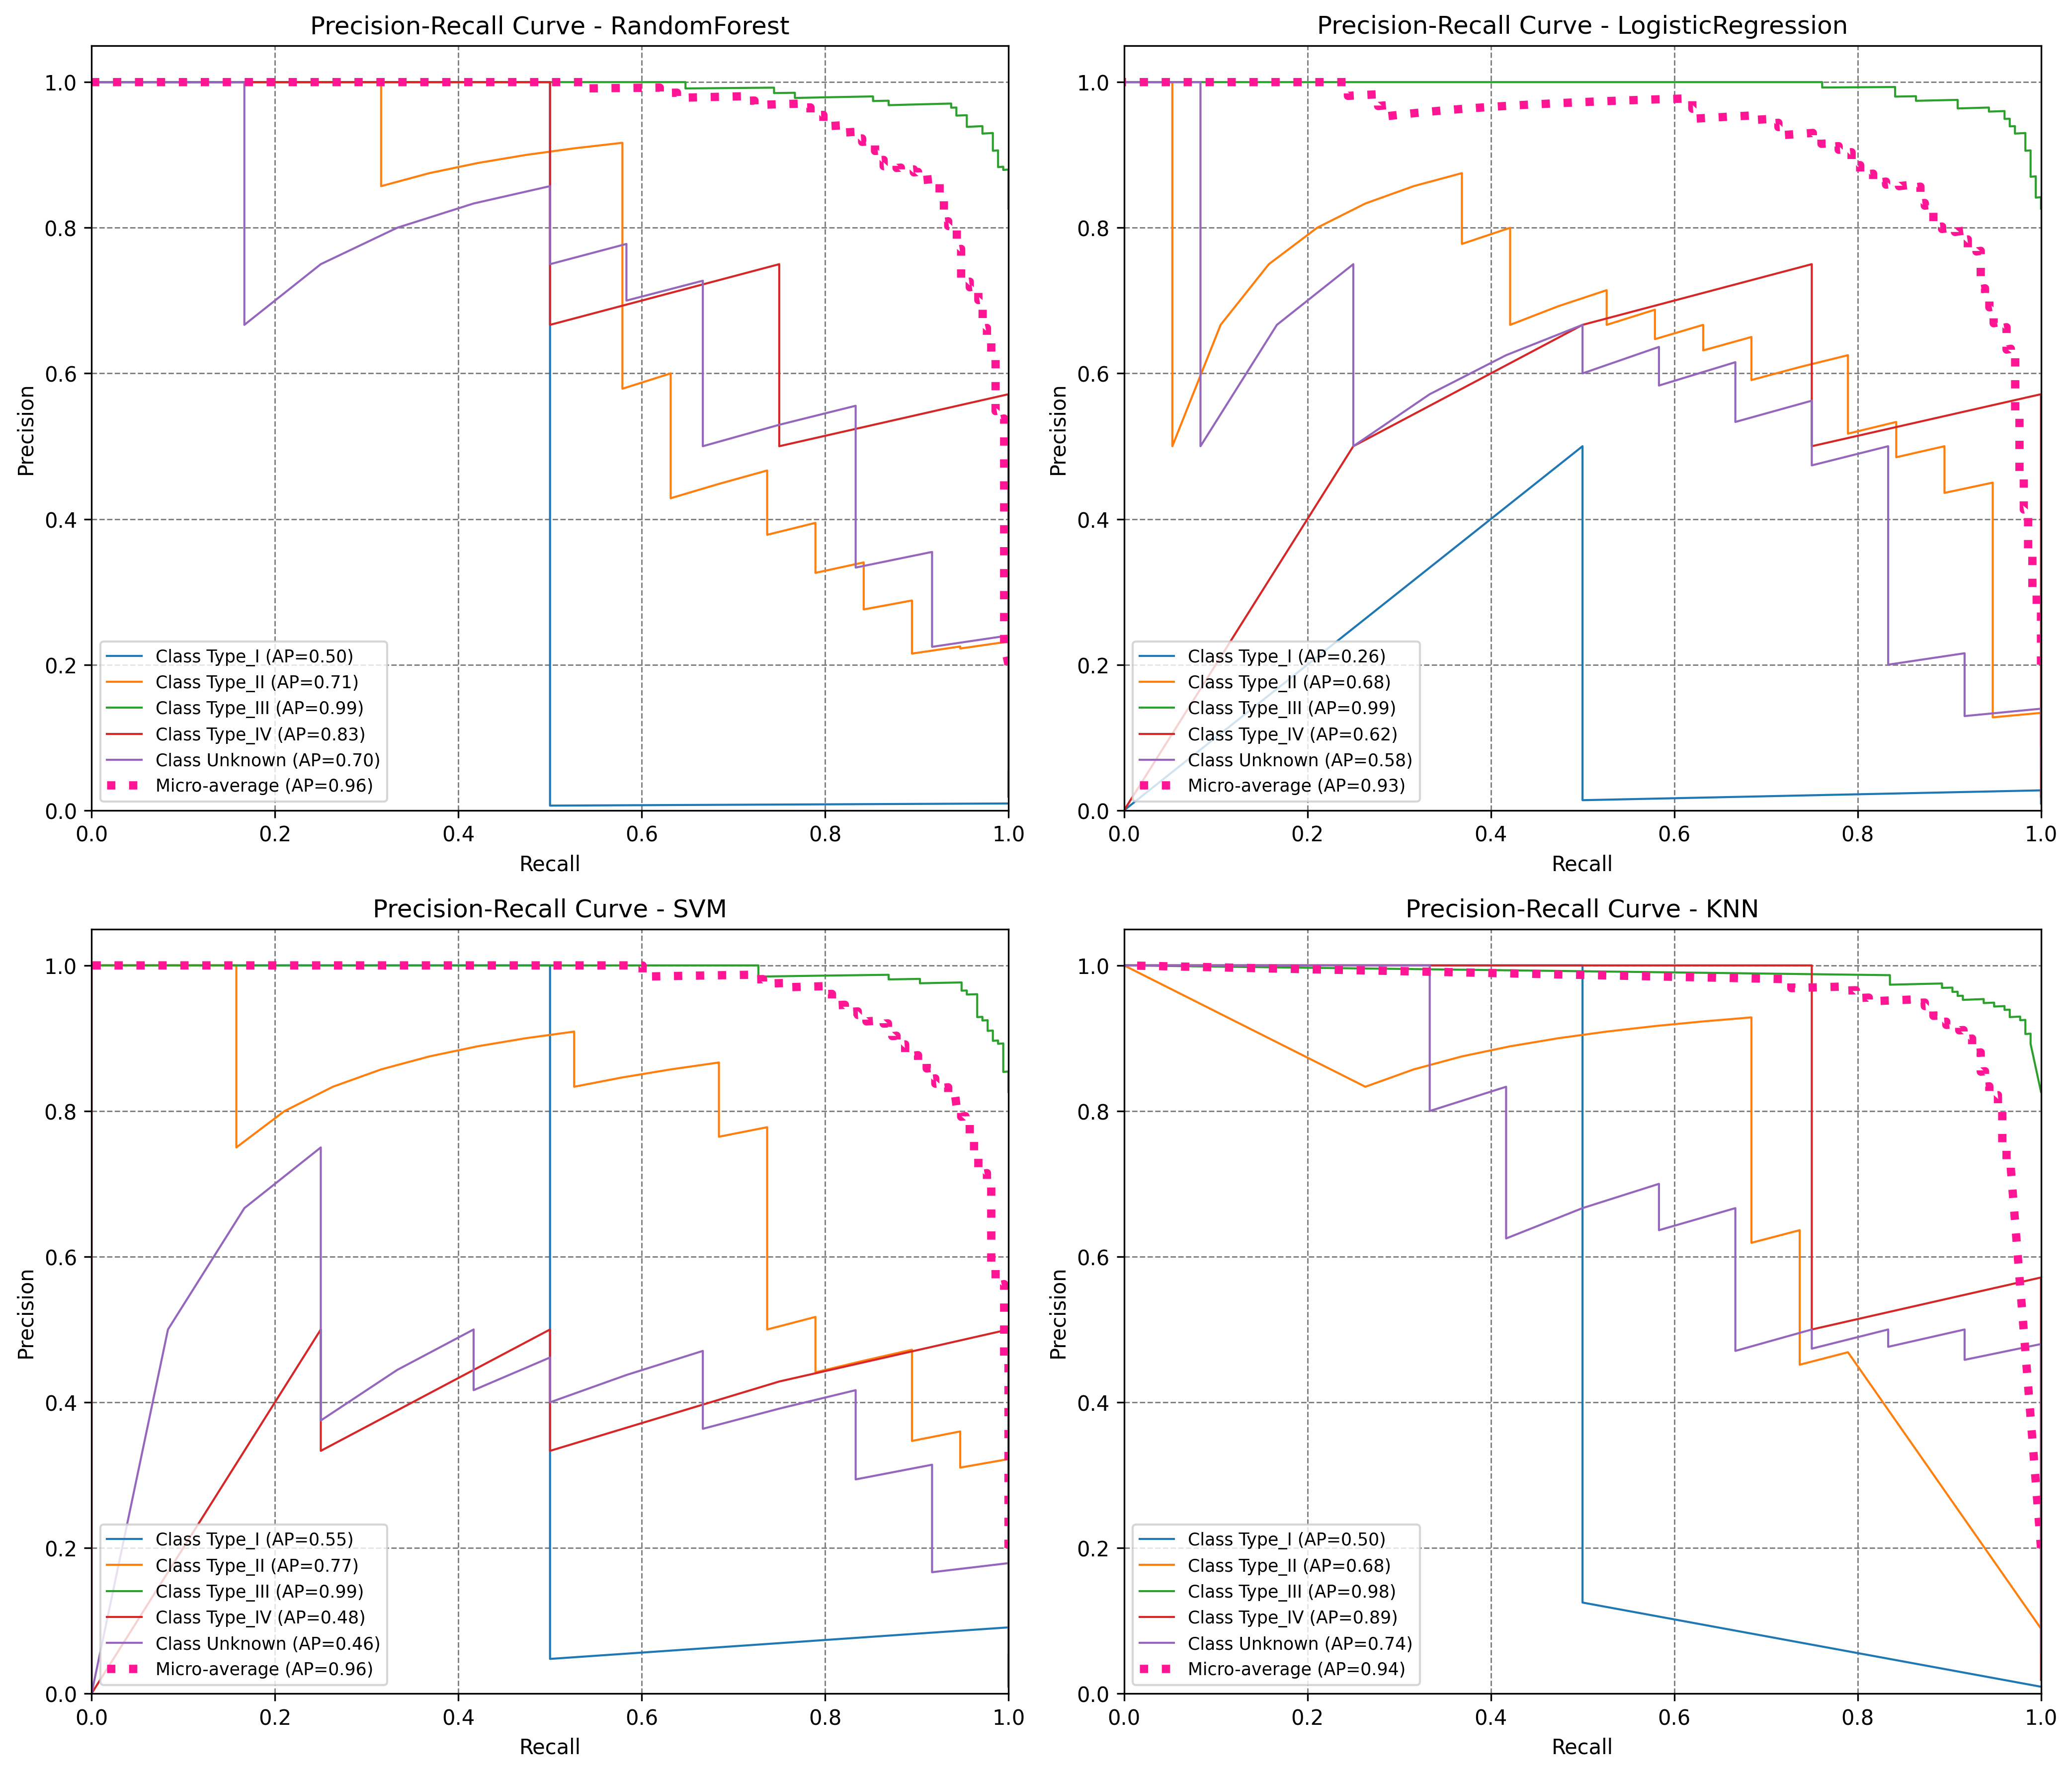
\includegraphics[width=0.7\textwidth]{images/2x2_precision_recall_curves_split_test_type.png}
	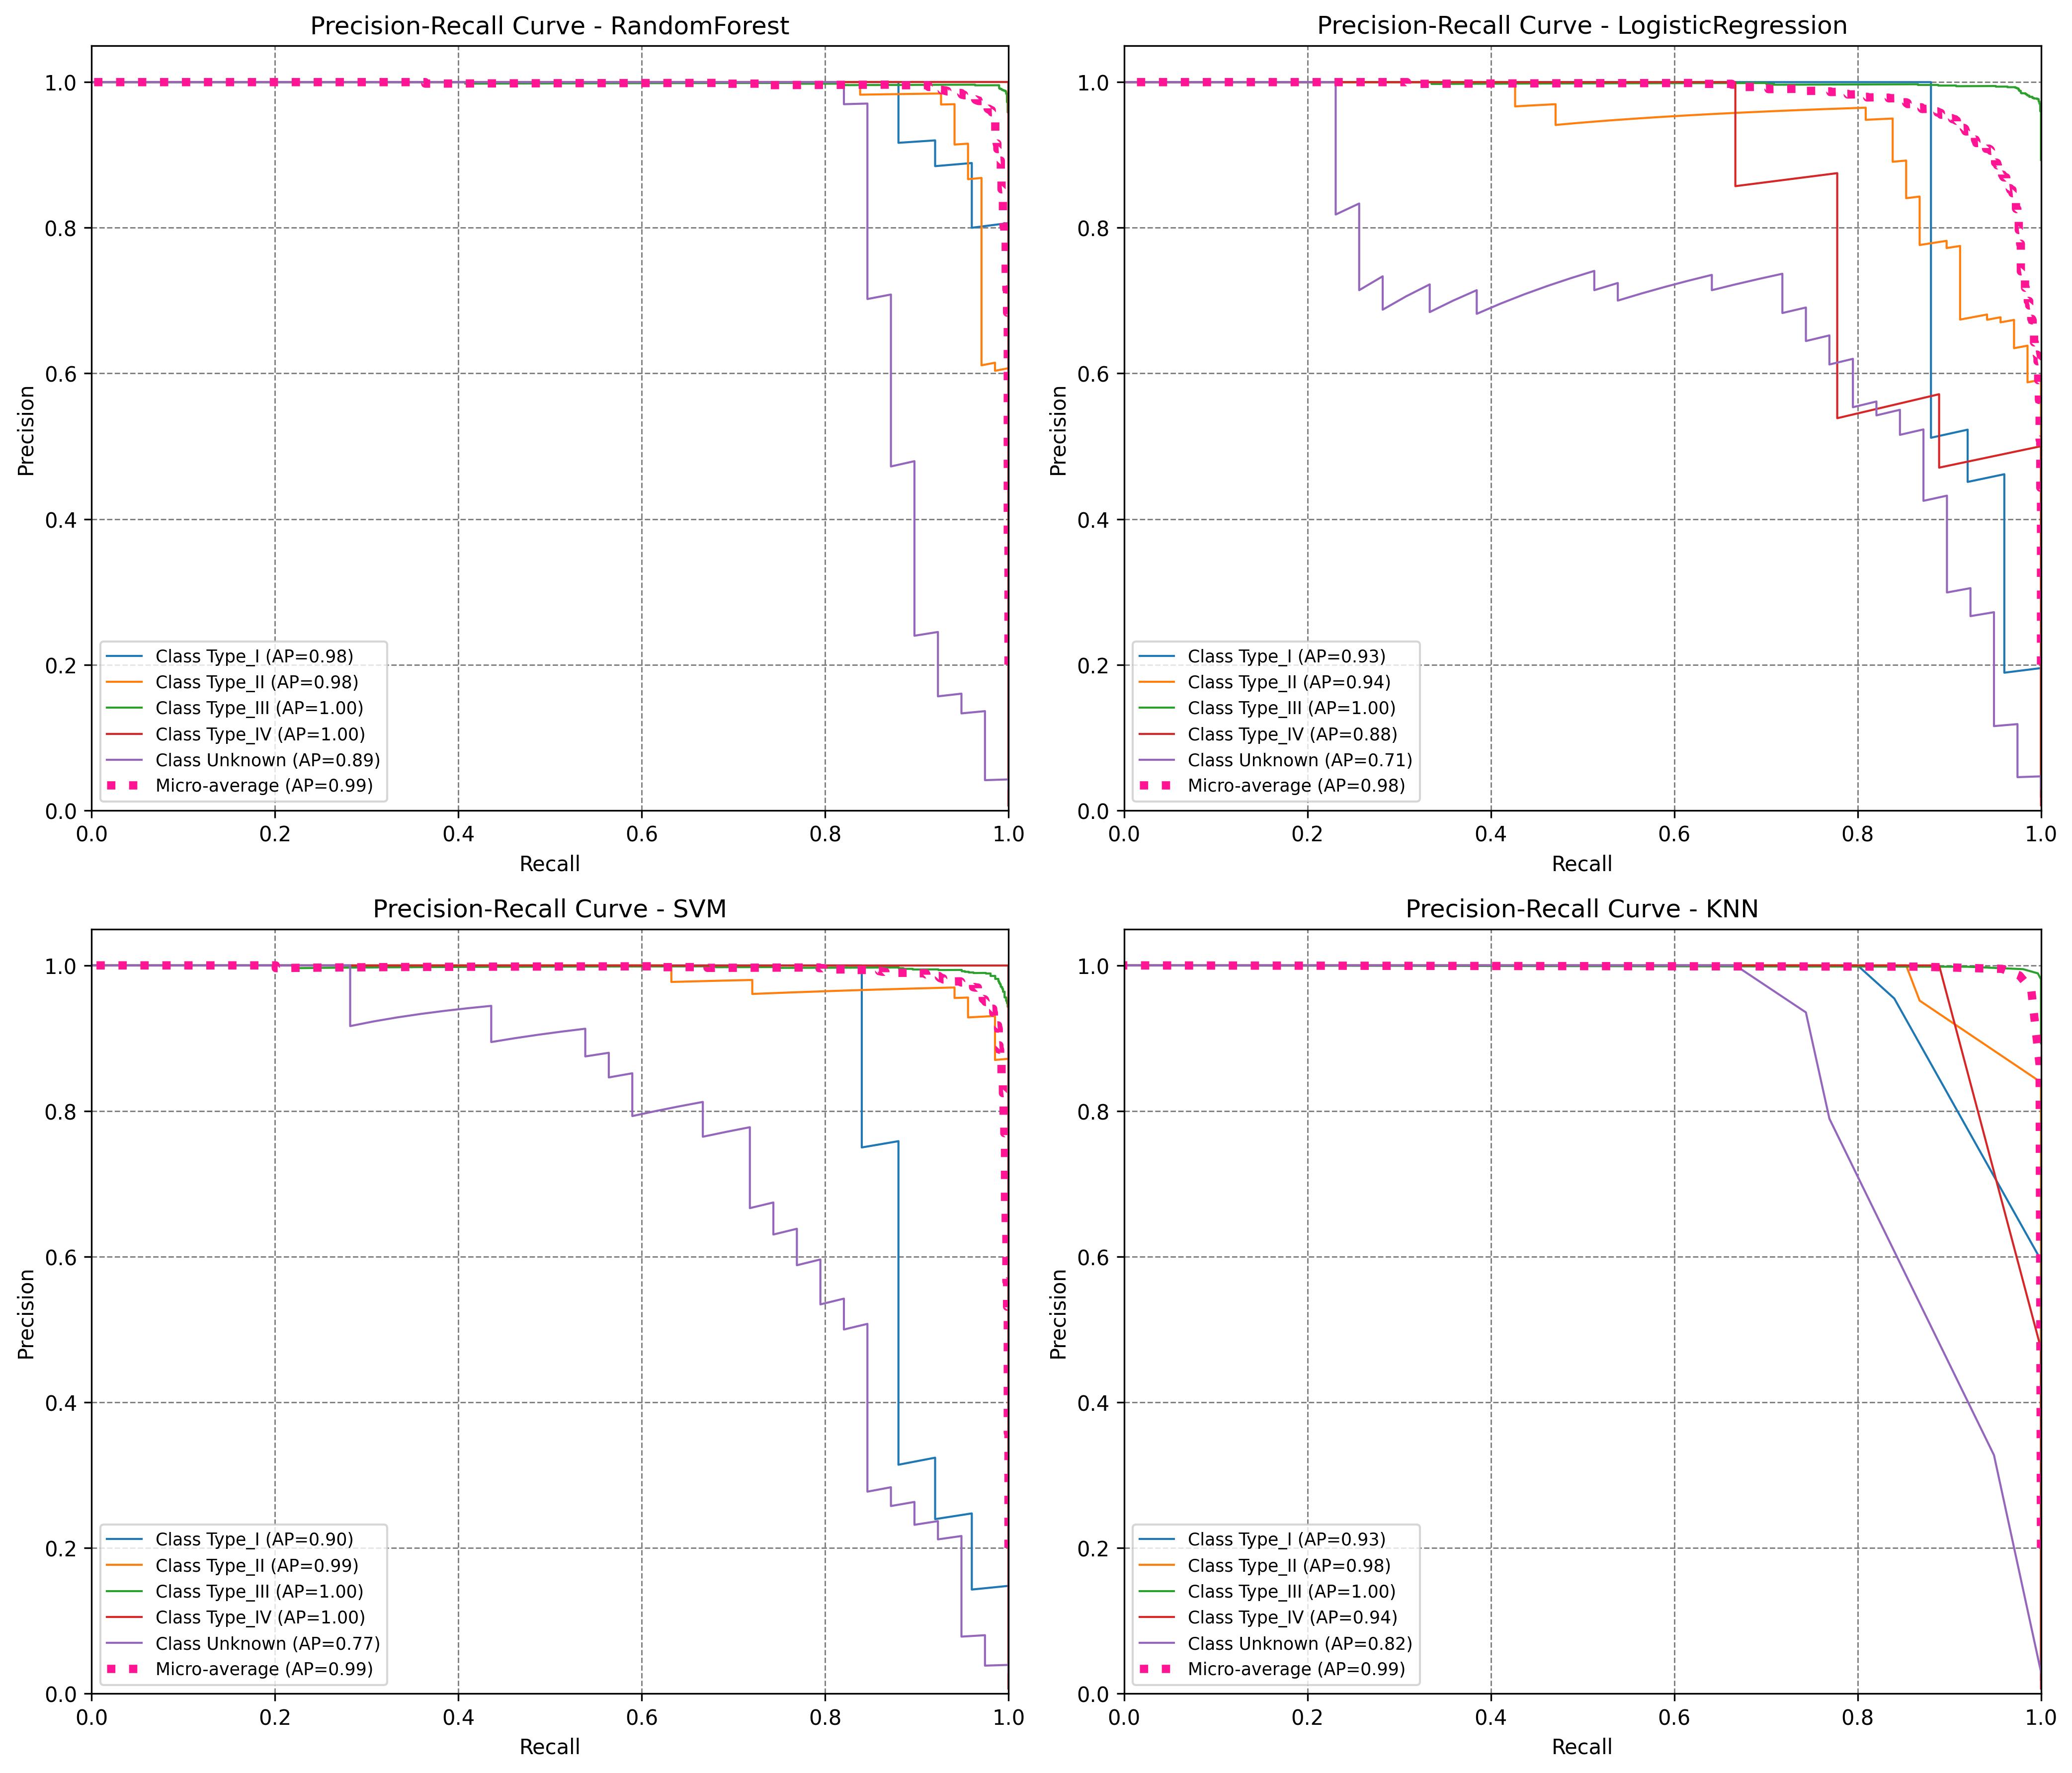
\includegraphics[width=0.7\textwidth]{images/2x2_precision_recall_curves_import_test_type.png}
	\caption{Precision-Recall Curves for Protein Sequence-Based Embeddings}
	\label{fig:pr_sequence}
\end{figure}

\subsubsection{Precision-Recall Curves for Protein Protein Fold-Based Embeddings}
\begin{figure}[H]
	\centering
	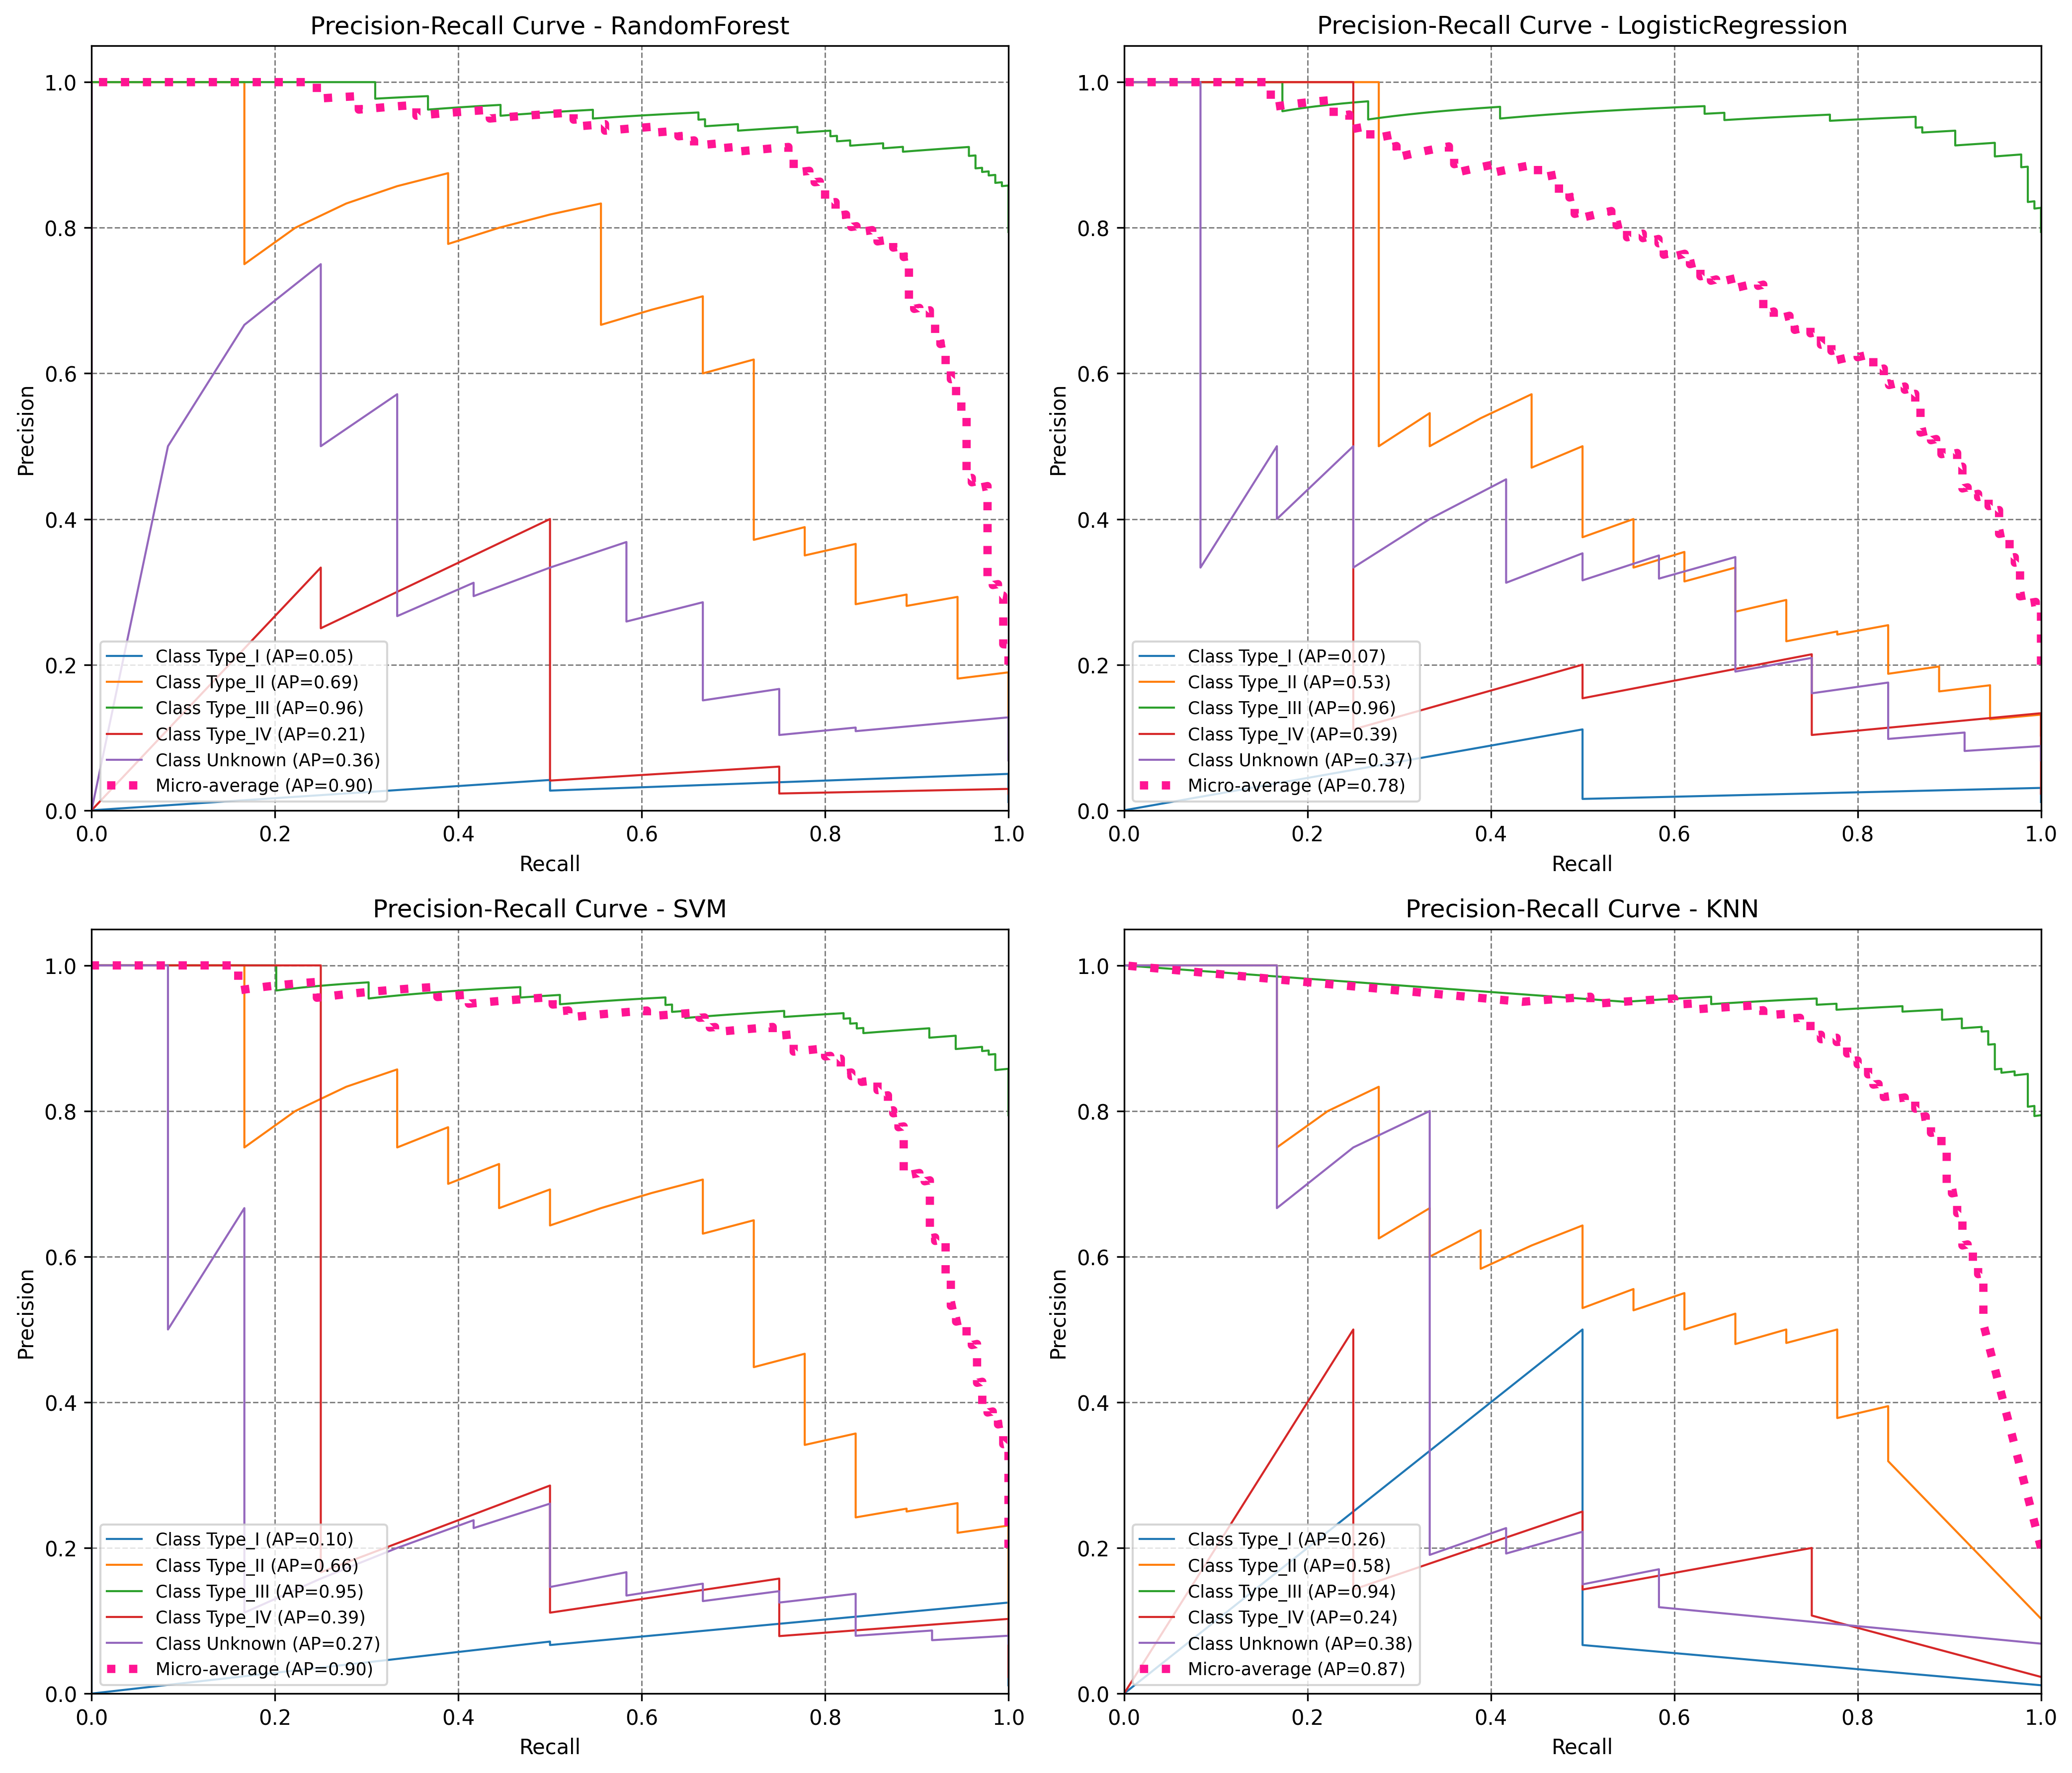
\includegraphics[width=0.7\textwidth]{images/2x2_precision_recall_curves_folds_test_split.png}
	\caption{Precision-Recall Curve for Protein Fold-Based Embeddings}
	\label{fig:pr_fold}
\end{figure}


%\subsubsection{Confusion Matrices for Protein Protein Sequence-Based Embeddings}
%\begin{figure}[h]
%	\centering
%	\begin{subfigure}{0.49\textwidth} 
%		\centering
%		\includegraphics[width=\linewidth]{images/conf_matrix_sequence1.jpg}
%		\caption{Confusion Matrix 1}
%	\end{subfigure}
%	\hfill
%	\begin{subfigure}{0.49\textwidth}
%		\centering
%		\includegraphics[width=\linewidth]{images/conf_matrix_sequence2.jpg}
%		\caption{Confusion Matrix 2}
%	\end{subfigure}
%	\caption{Confusion Matrices for Protein Sequence-Based Embeddings}
%	\label{fig:conf_matrix_sequence}
%\end{figure}



%\subsubsection{Confusion Matrices for Protein Protein Fold-Based Embeddings}
%\begin{figure}[h]
%	\centering
%	\includegraphics[width=0.7\textwidth]{images/conf_matrix_fold.jpg}
%	\caption{Confusion Matrix for Protein Fold-Based Embeddings}
%	\label{fig:conf_matrix_fold}
%\end{figure}

\subsection{ExoTarget Predictor}
\subsection{Model Training}

\subsubsection{Learning Curves for Protein Sequence-Based Embeddings}
\begin{figure}[H]
	\centering
	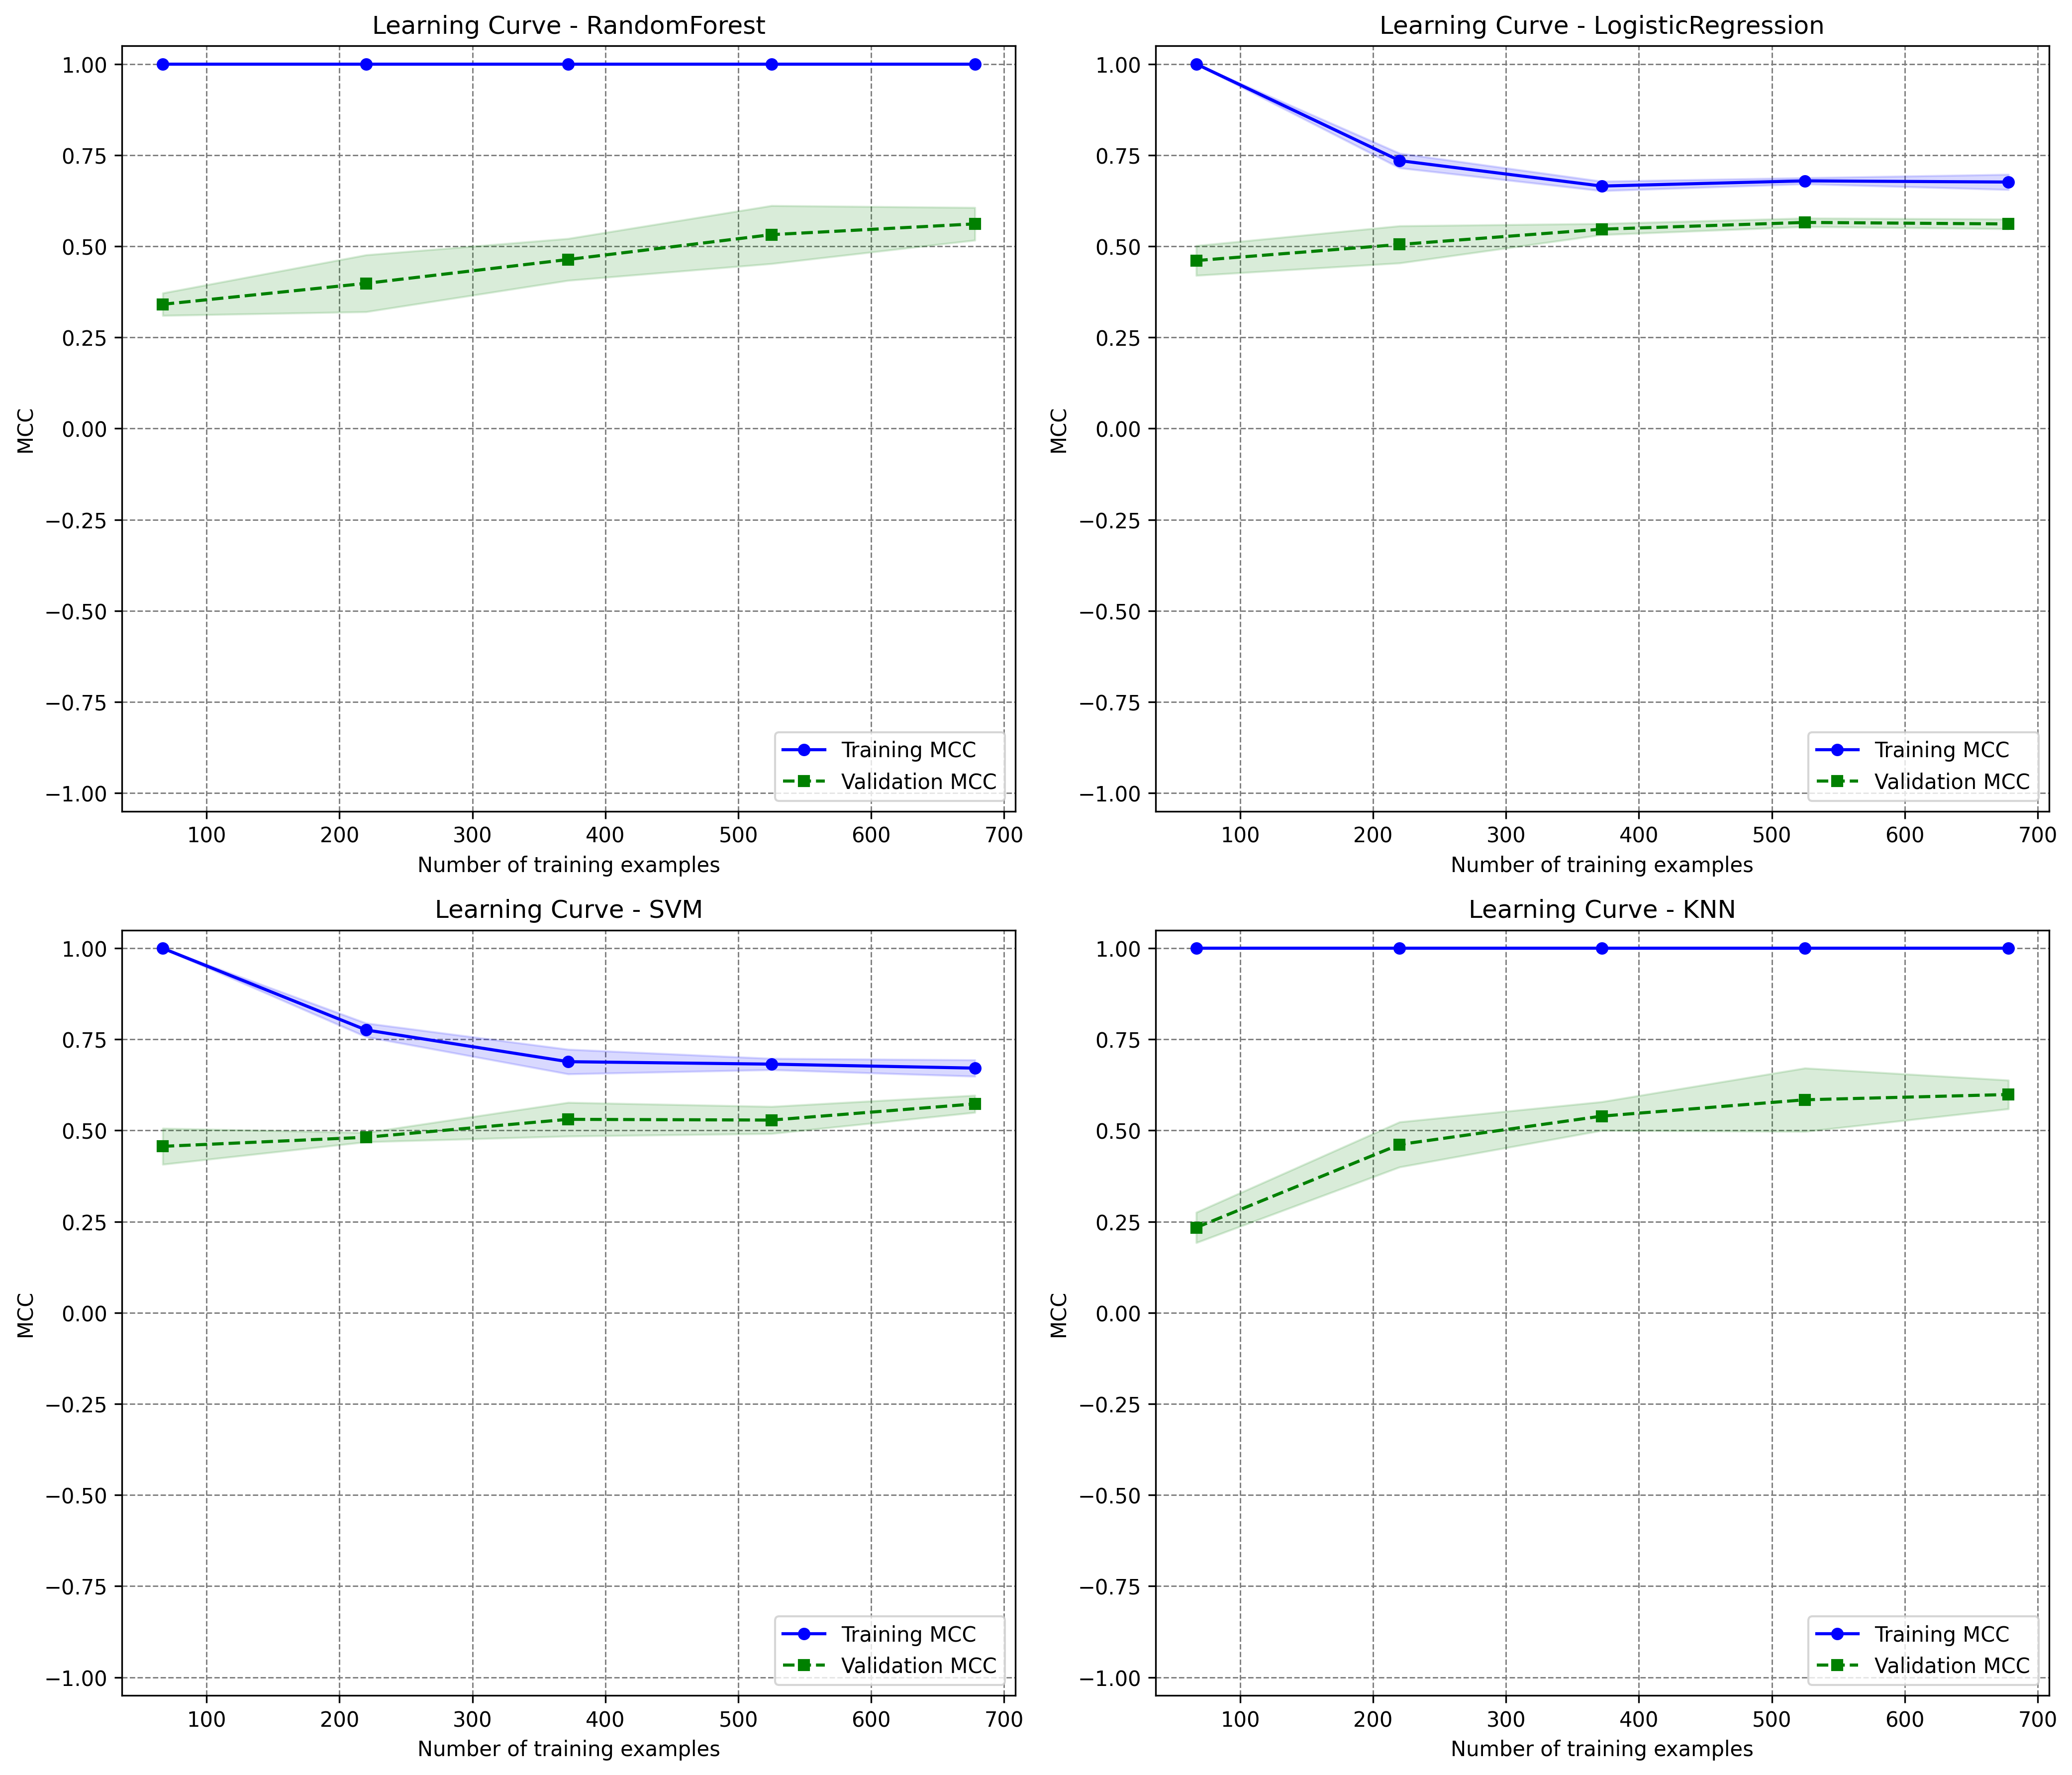
\includegraphics[width=0.9\textwidth]{images/2x2_learning_curves_split_test_target.png}
	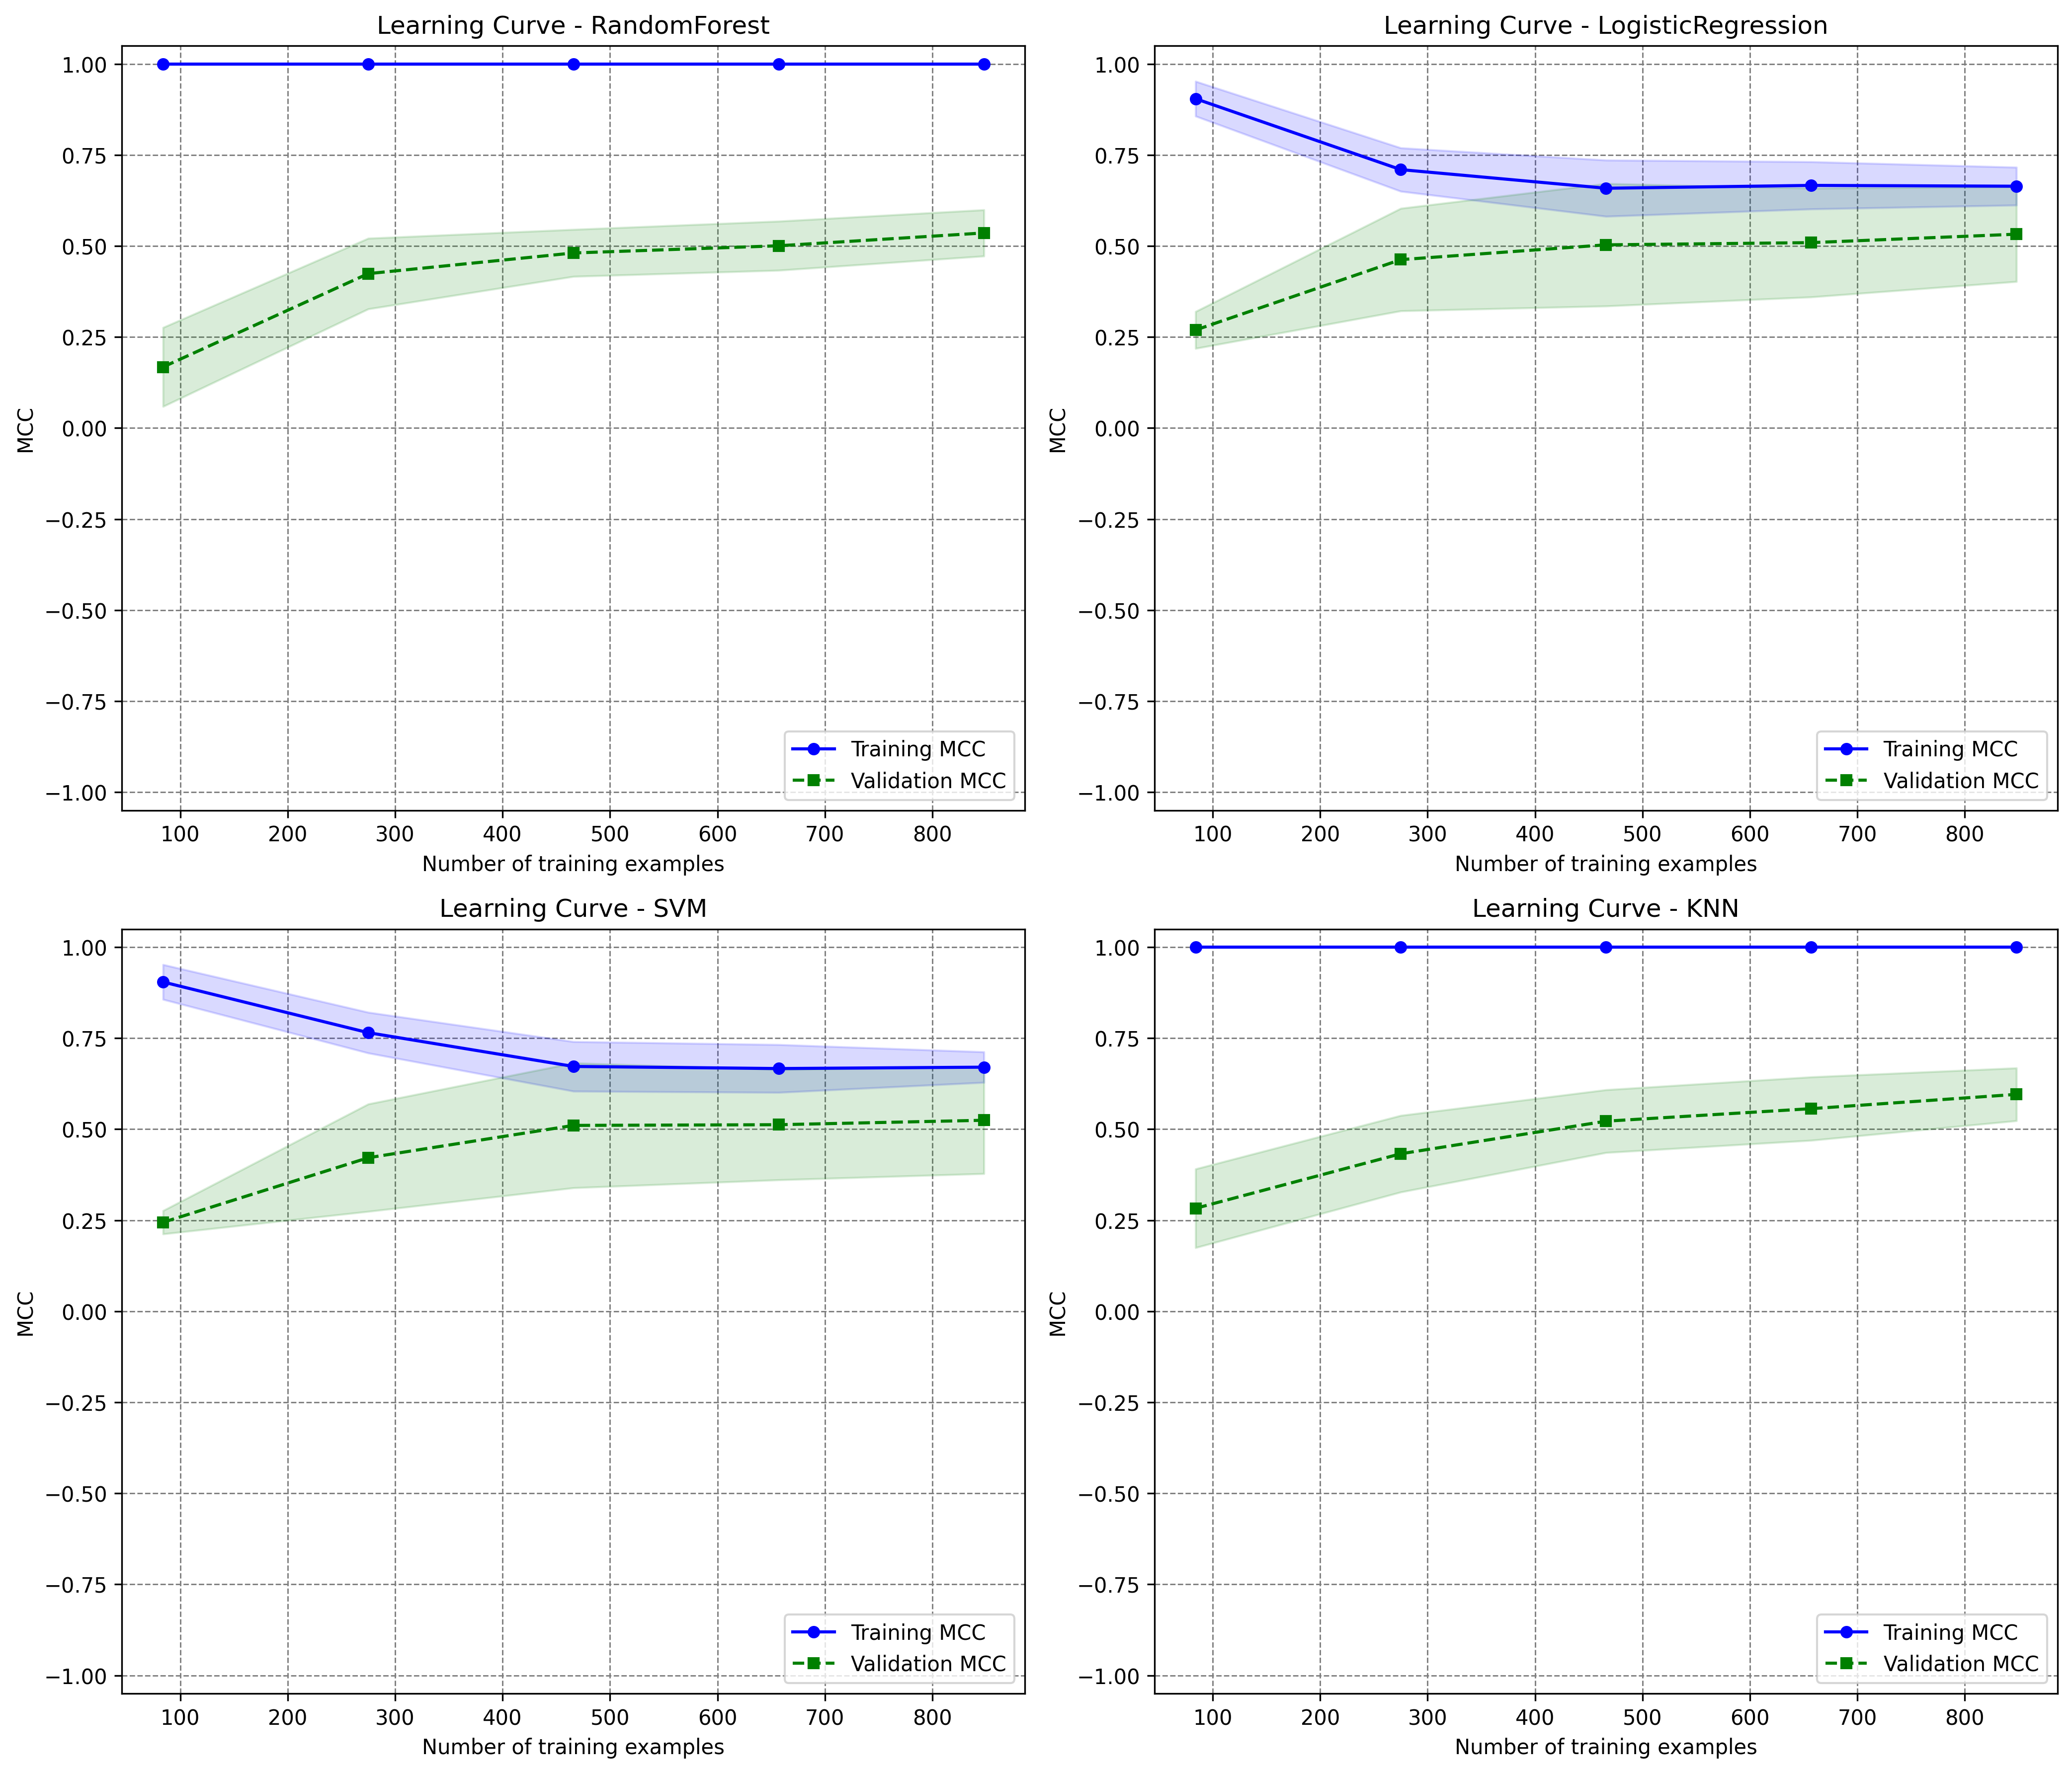
\includegraphics[width=0.9\textwidth]{images/2x2_learning_curves_import_test_target.png}
	\caption{Learning Curves for Protein Sequence-Based Embeddings}
	\label{fig:sequence_learning_curves}
\end{figure}

\subsubsection{Learning Curves for Protein Protein Fold-Based Embeddings}
\begin{figure}[H]
	\centering
	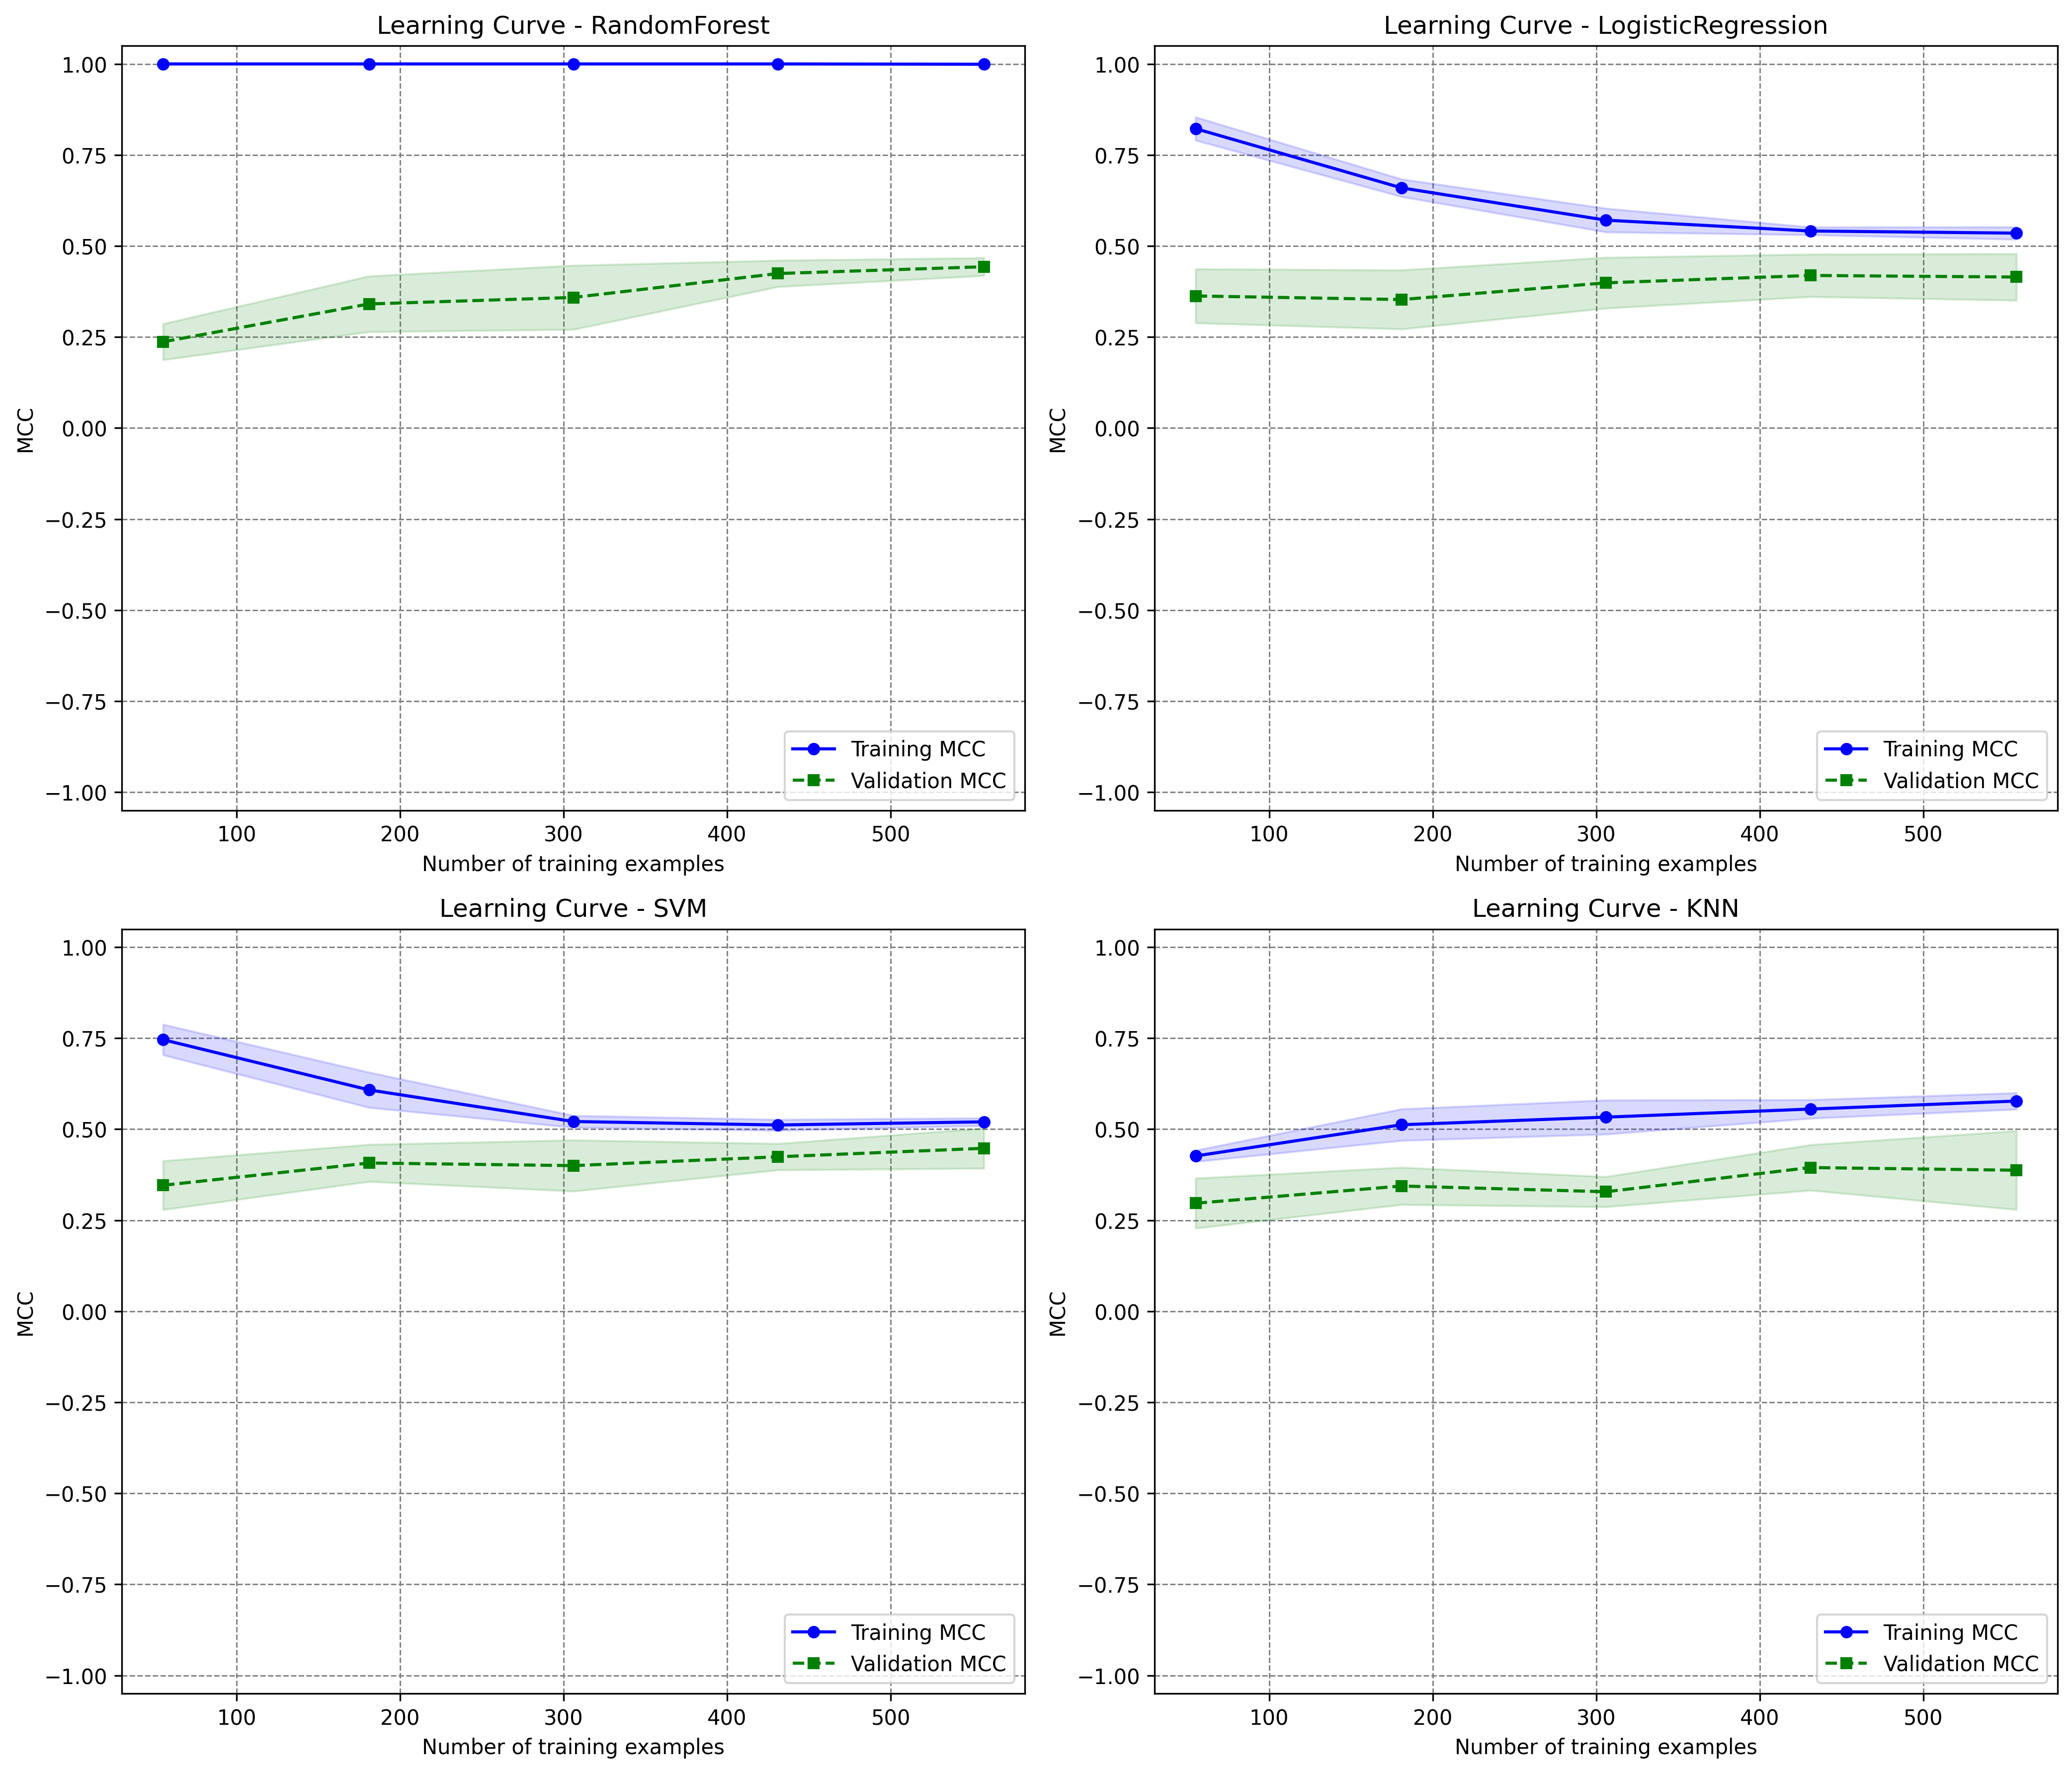
\includegraphics[width=1.1\textwidth]{images/2x2_learning_curves_target_folds_test_split.png}
	\caption{Learning Curve for Protein Fold-Based Embeddings}
	\label{fig:fold_learning_curve}
\end{figure}

\subsection{Performance Evaluation}

\subsubsection{MCC Bar Plots for Protein Sequence-Based Embeddings}
\begin{figure}[H]
	\centering
	\begin{subfigure}{0.49\textwidth}
		\centering
		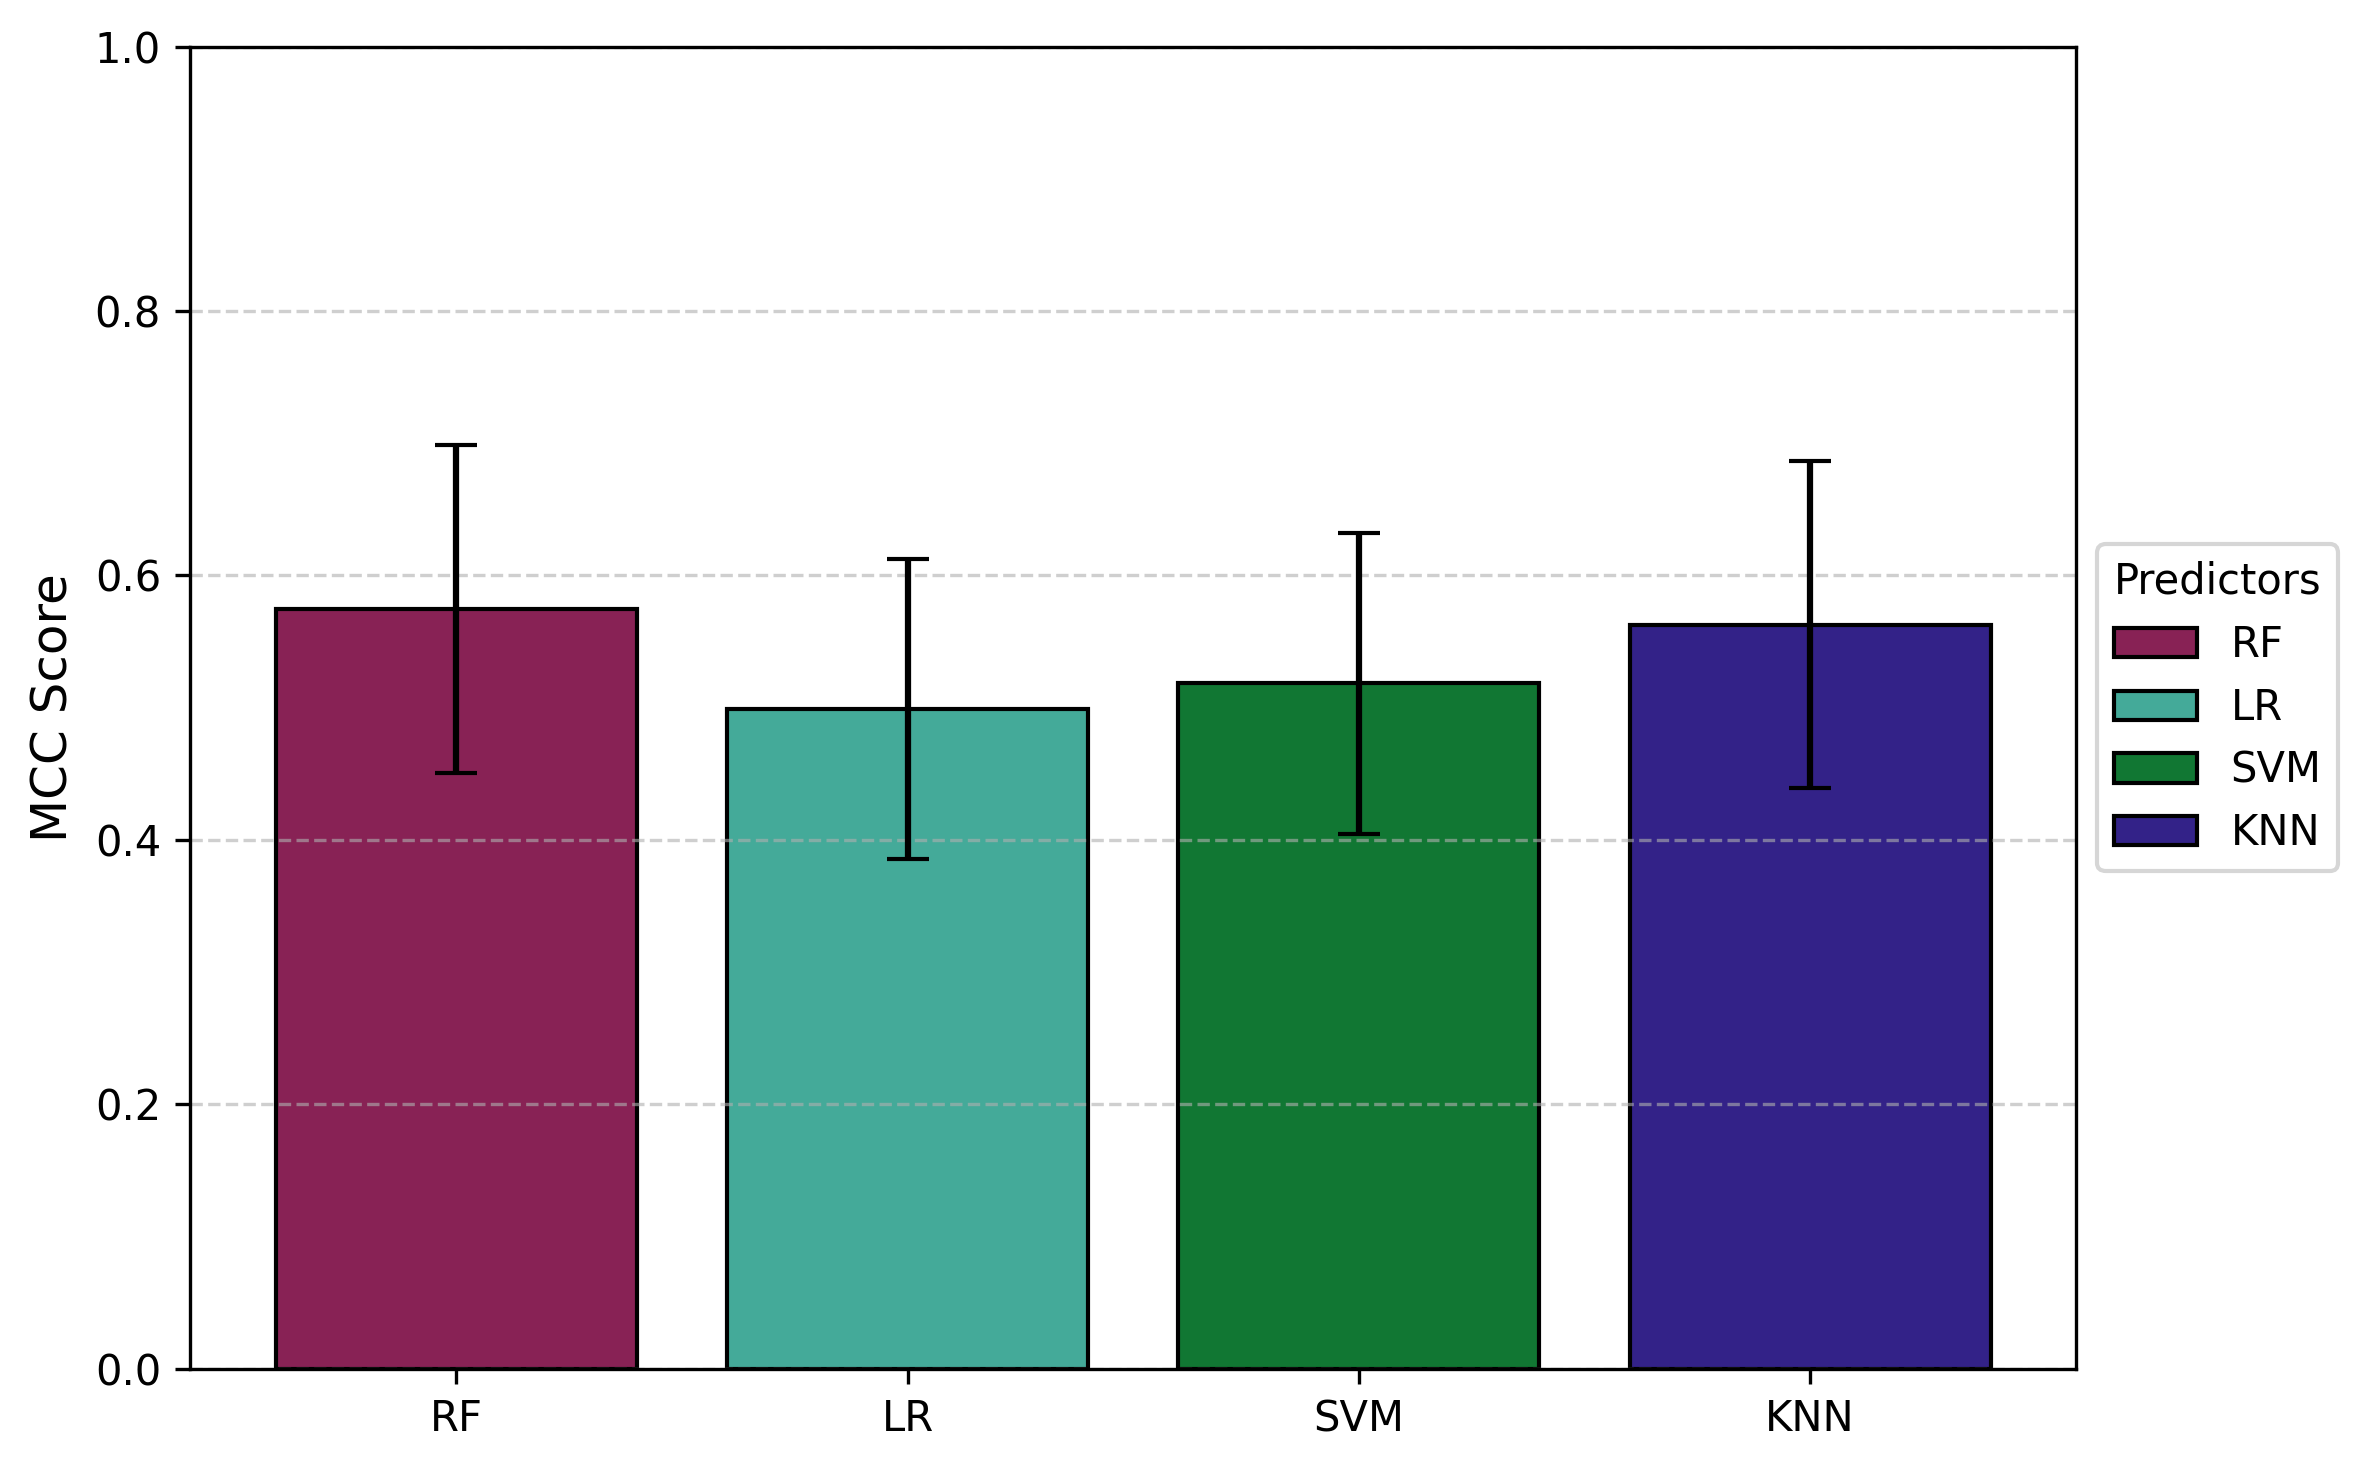
\includegraphics[width=\linewidth]{images/comparison_graph_with_error_bars_split_test_target.png}
		\caption{MCC Plot 1}
	\end{subfigure}
	\hfill
	\begin{subfigure}{0.49\textwidth}
		\centering
		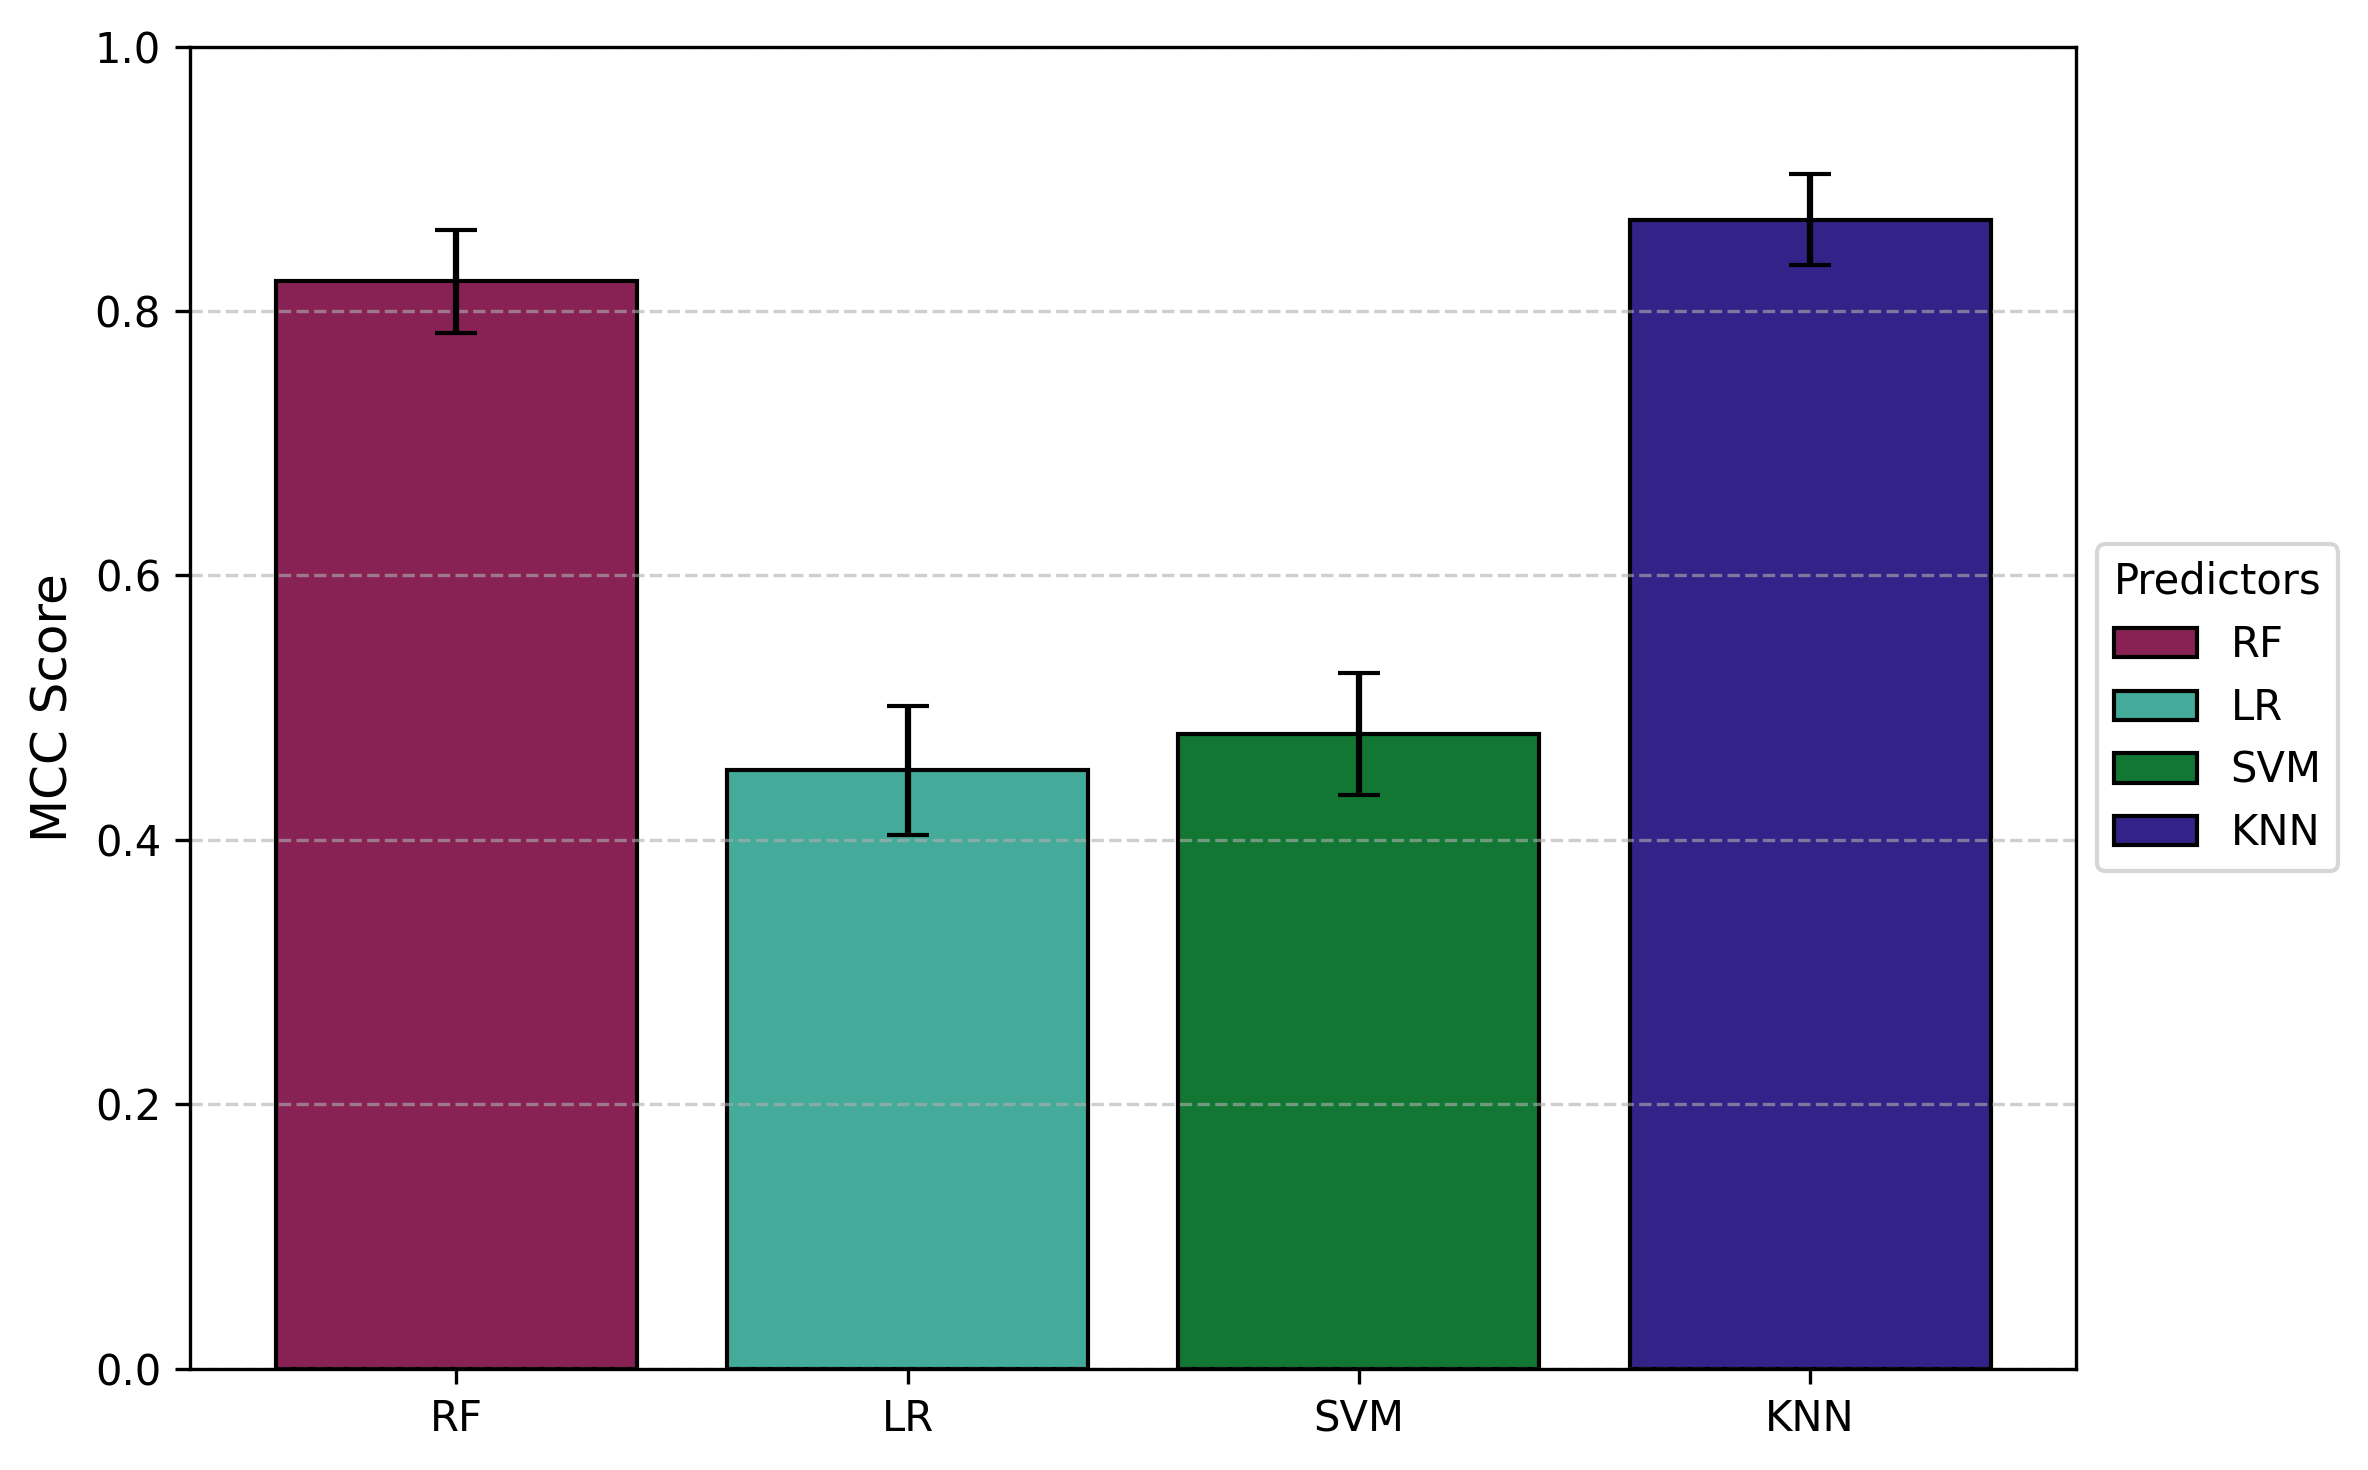
\includegraphics[width=\linewidth]{images/comparison_graph_with_error_bars_import_test_target.png}
		\caption{MCC Plot 2}
	\end{subfigure}
	\caption{MCC Bar Plots for Protein Sequence-Based Embeddings}
	\label{fig:mcc_sequence}
\end{figure}

\subsubsection{MCC Bar Plots for Protein Protein Fold-Based Embeddings}
\begin{figure}[H]
	\centering
	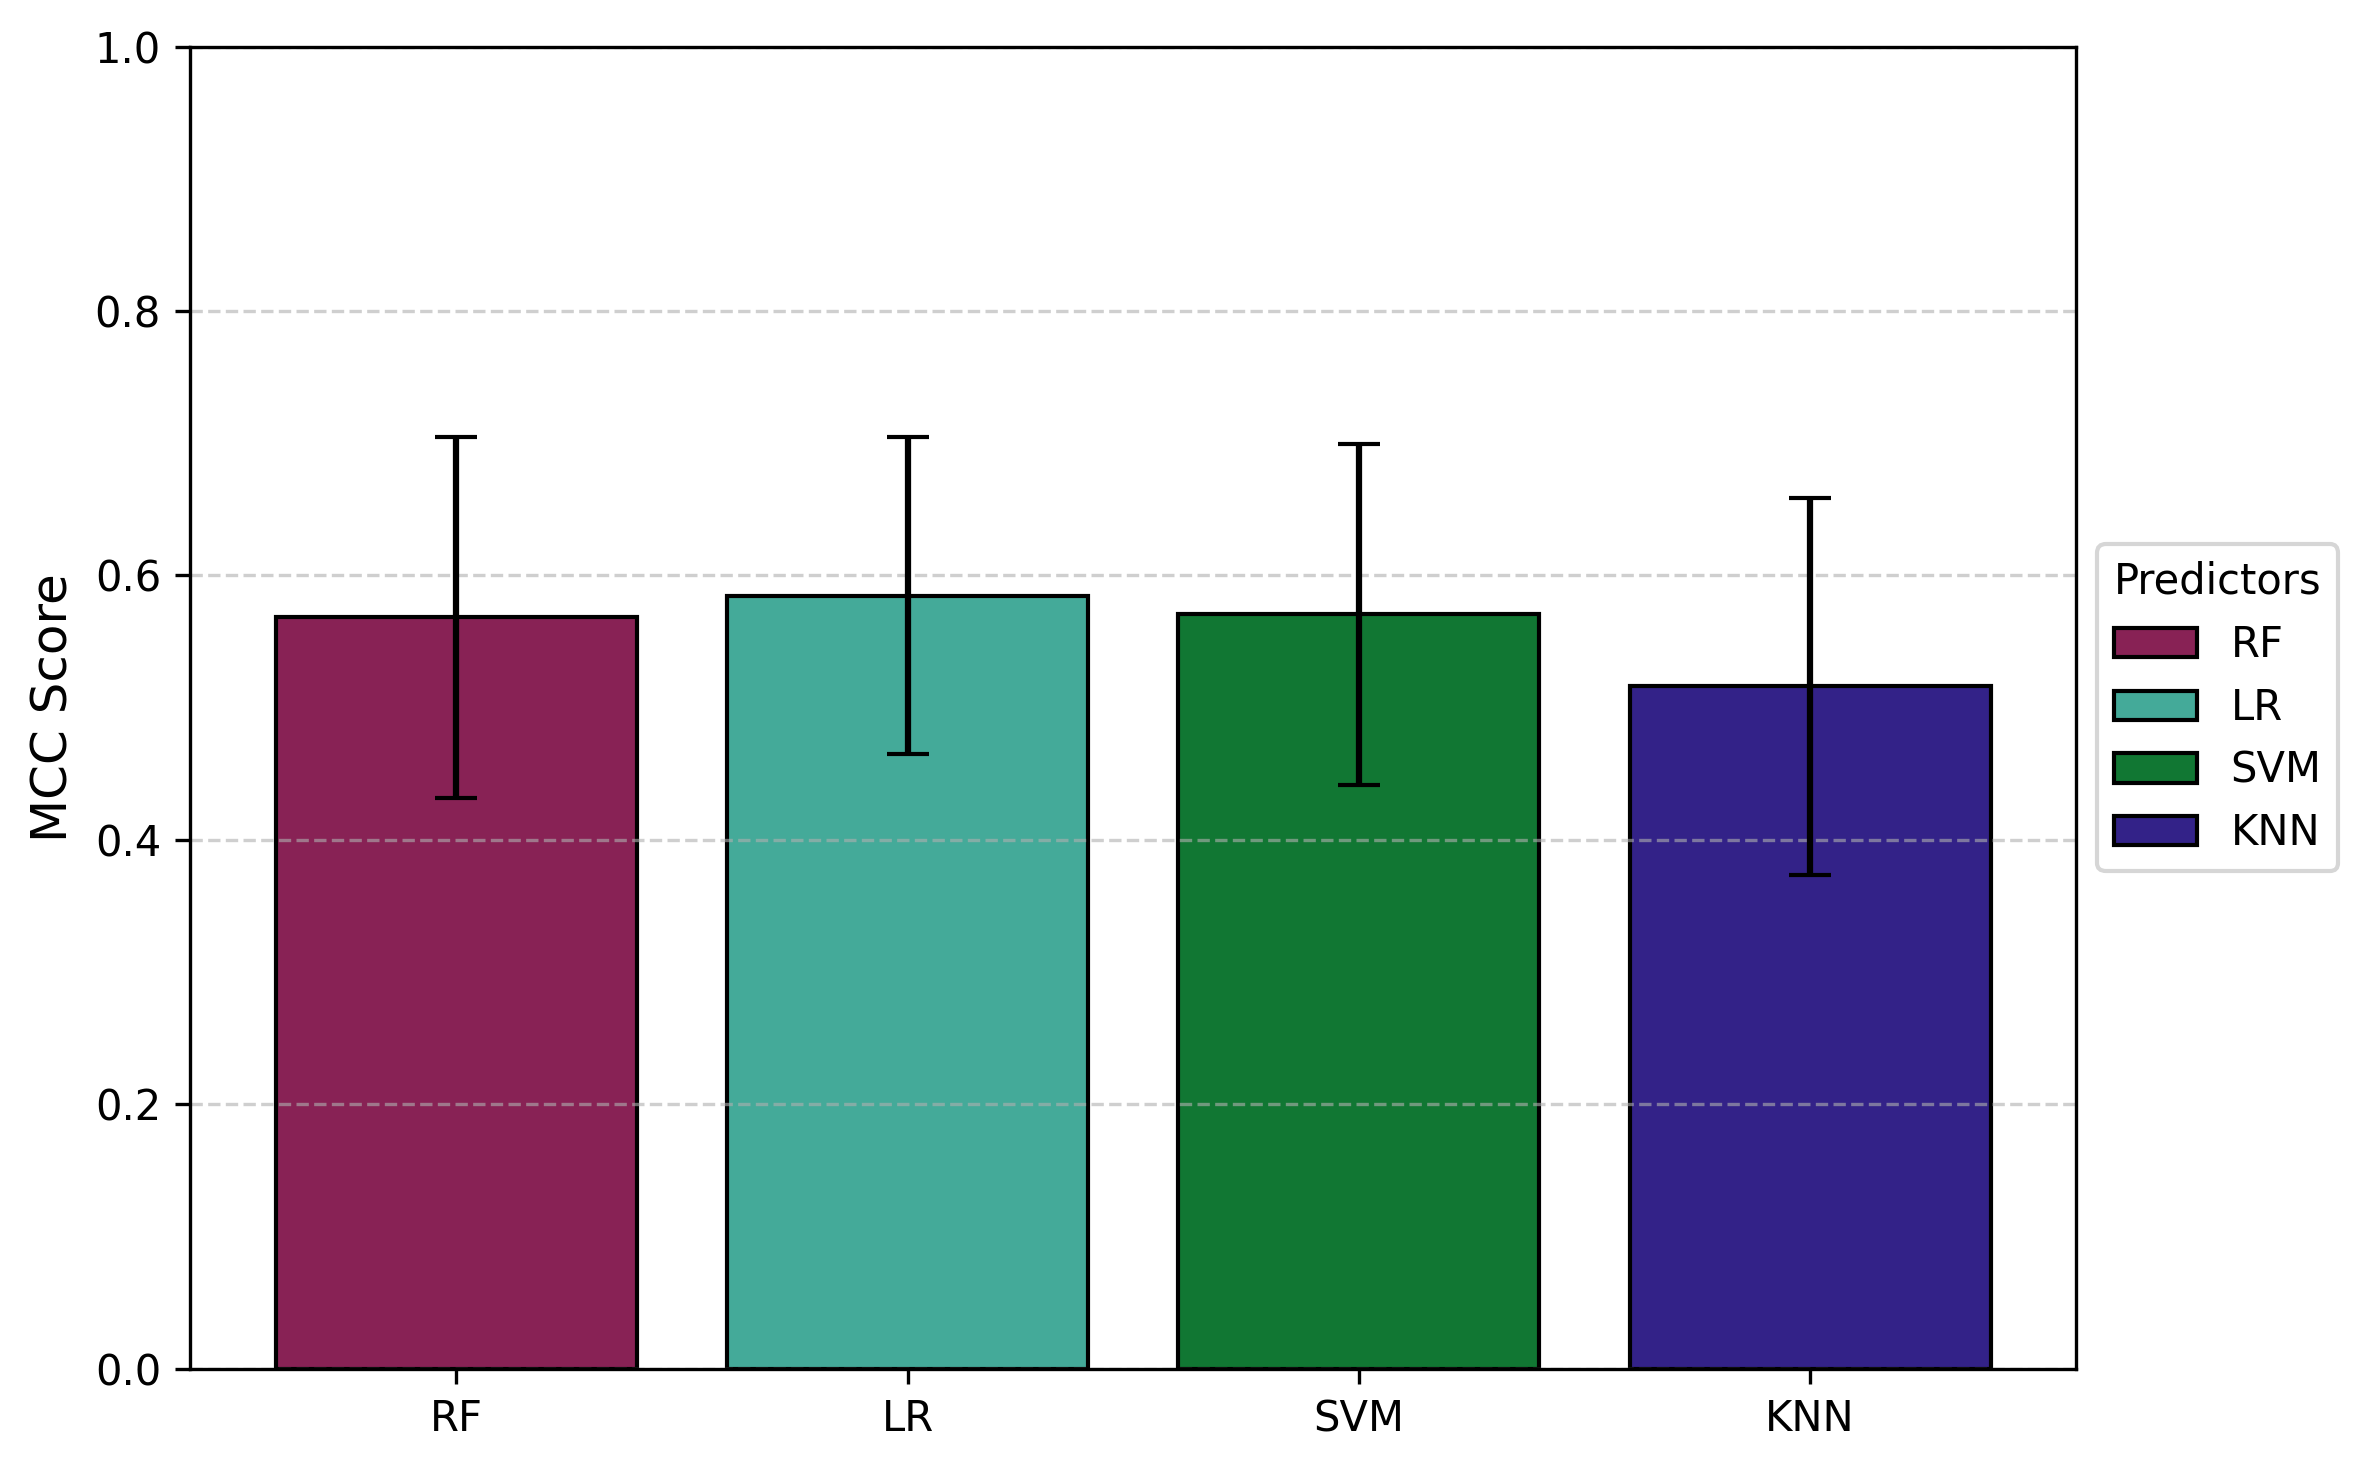
\includegraphics[width=0.7\textwidth]{images/comparison_graph_with_error_bars_target_folds_test_split.png}
	\caption{MCC Bar Plot for Protein Fold-Based Embeddings}
	\label{fig:mcc_fold}
\end{figure}

\subsubsection{ROC Curves for Protein Sequence-Based Embeddings}
\begin{figure}[H]
	\centering
	\begin{subfigure}{0.49\textwidth}
		\centering
		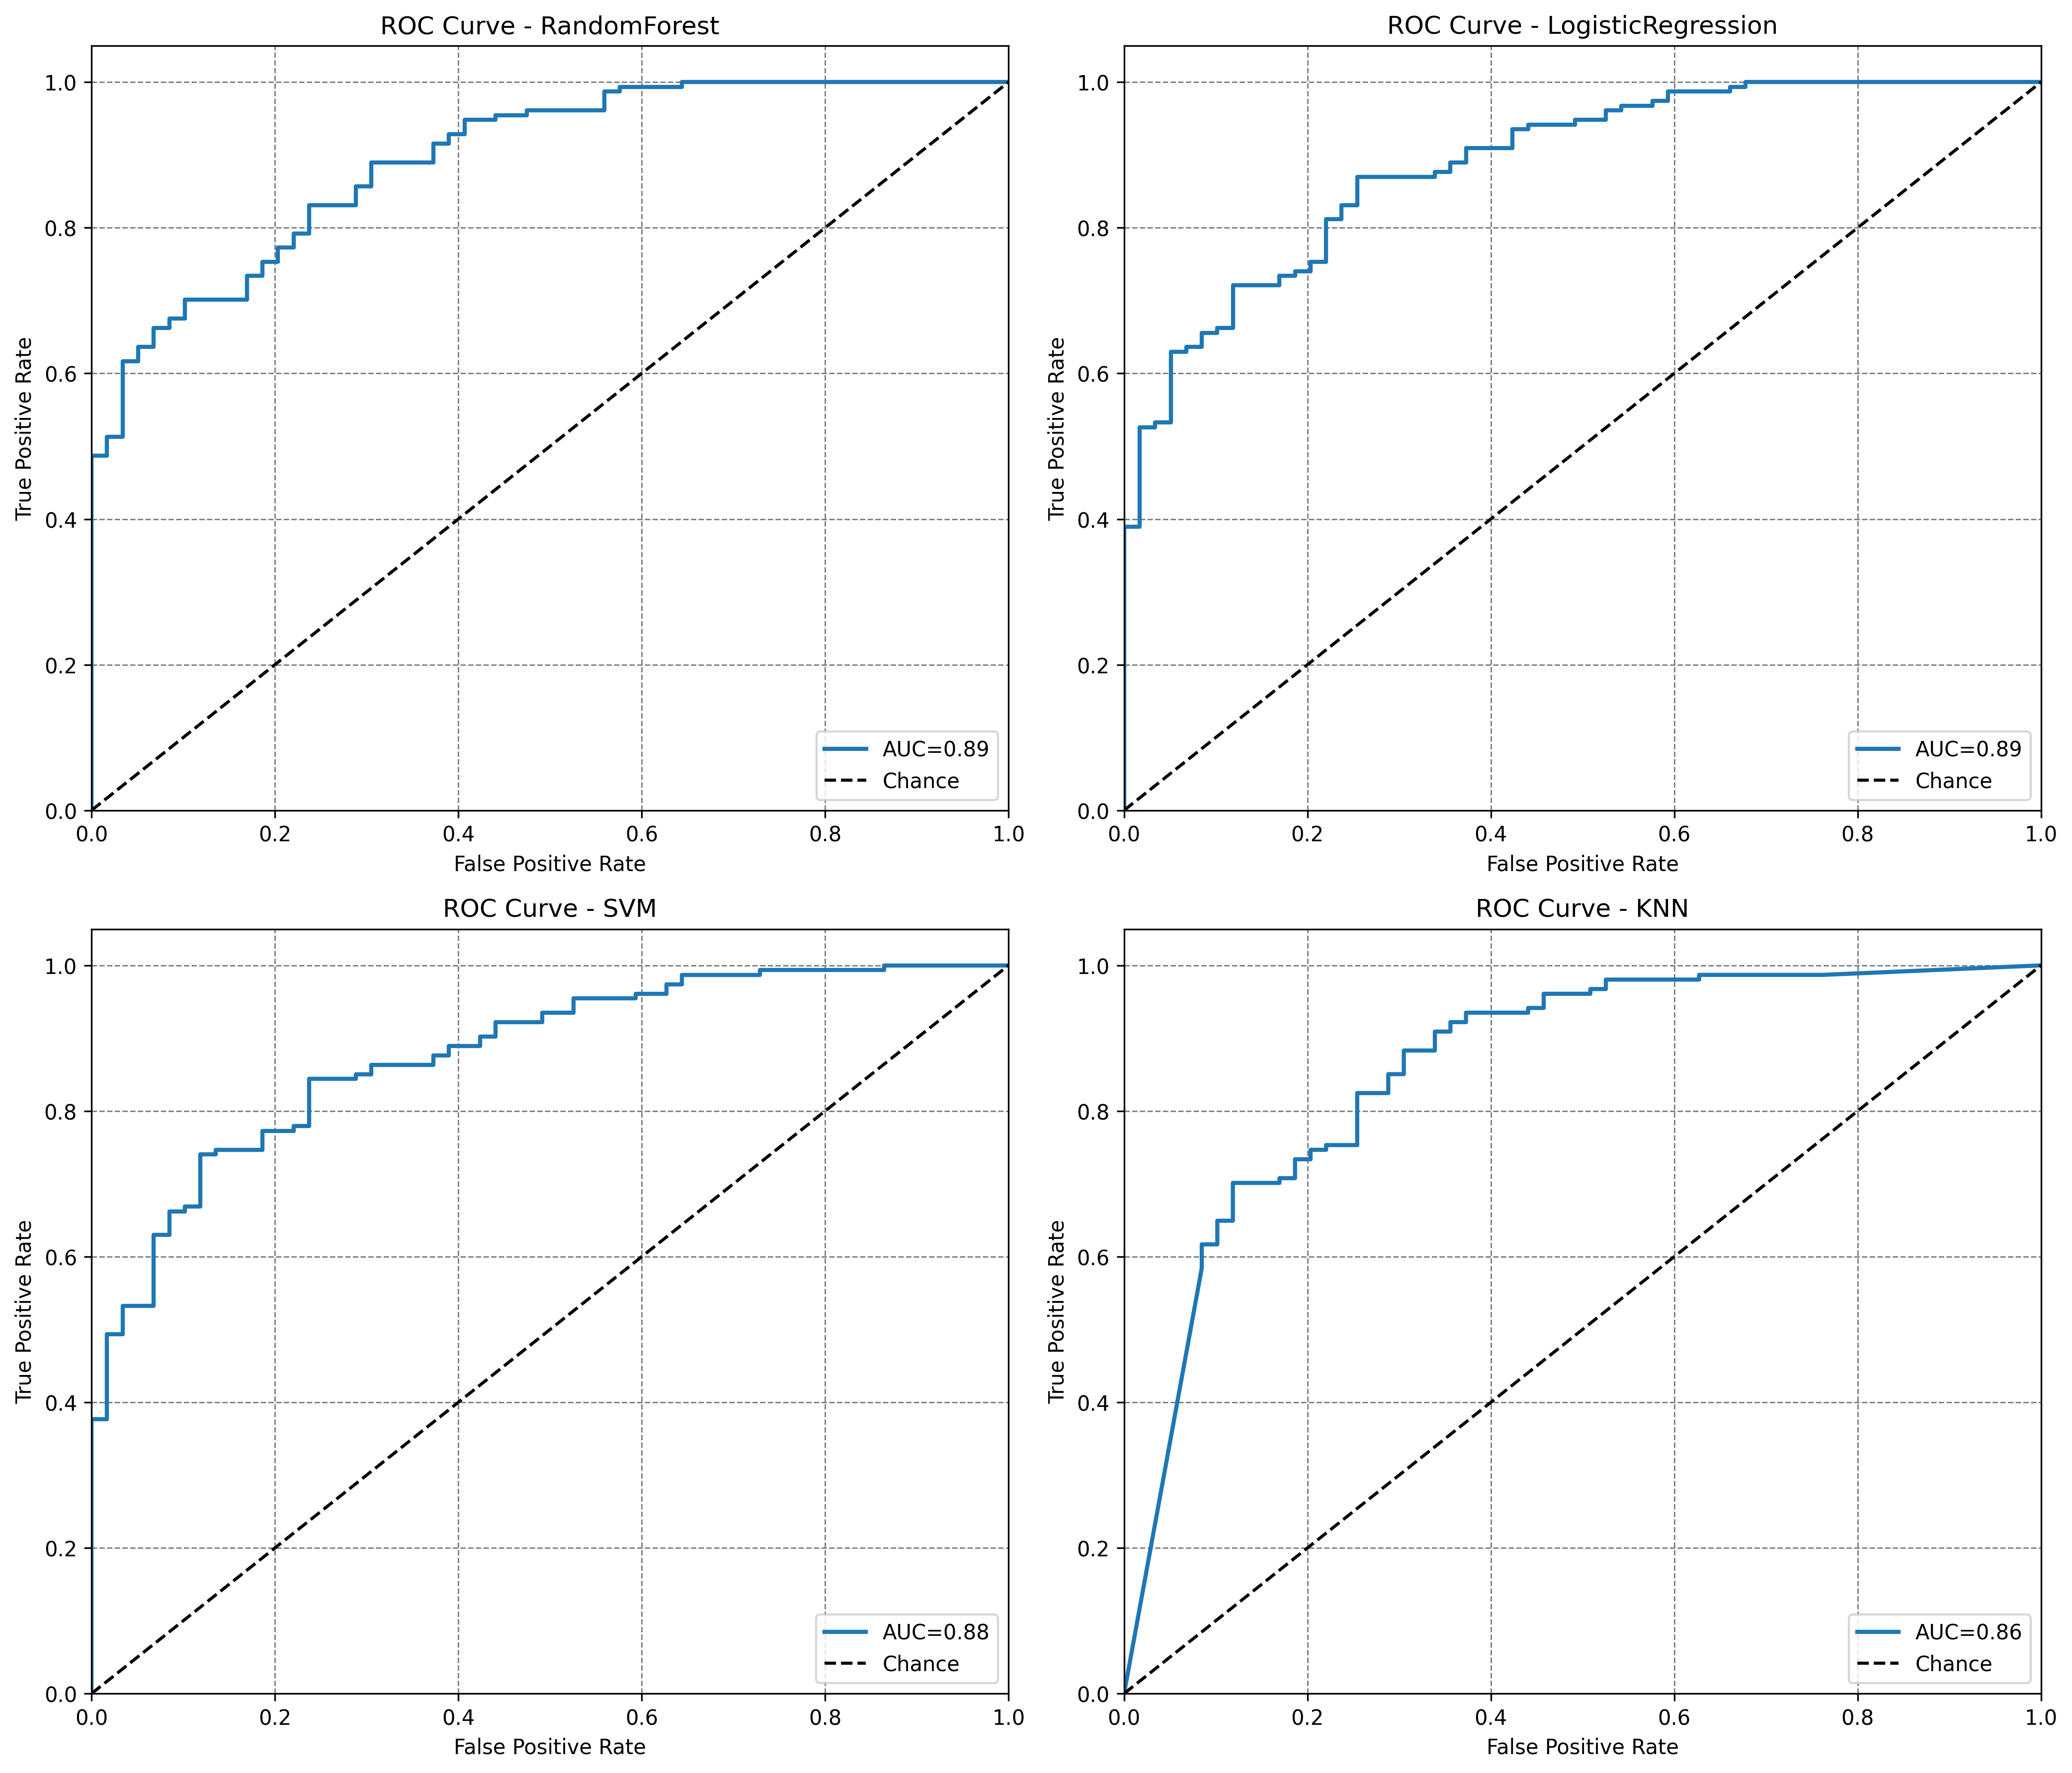
\includegraphics[width=\linewidth]{images/2x2_roc_curves_split_test_target.png}
		\caption{ROC Curve 1}
	\end{subfigure}
	\hfill
	\begin{subfigure}{0.49\textwidth}
		\centering
		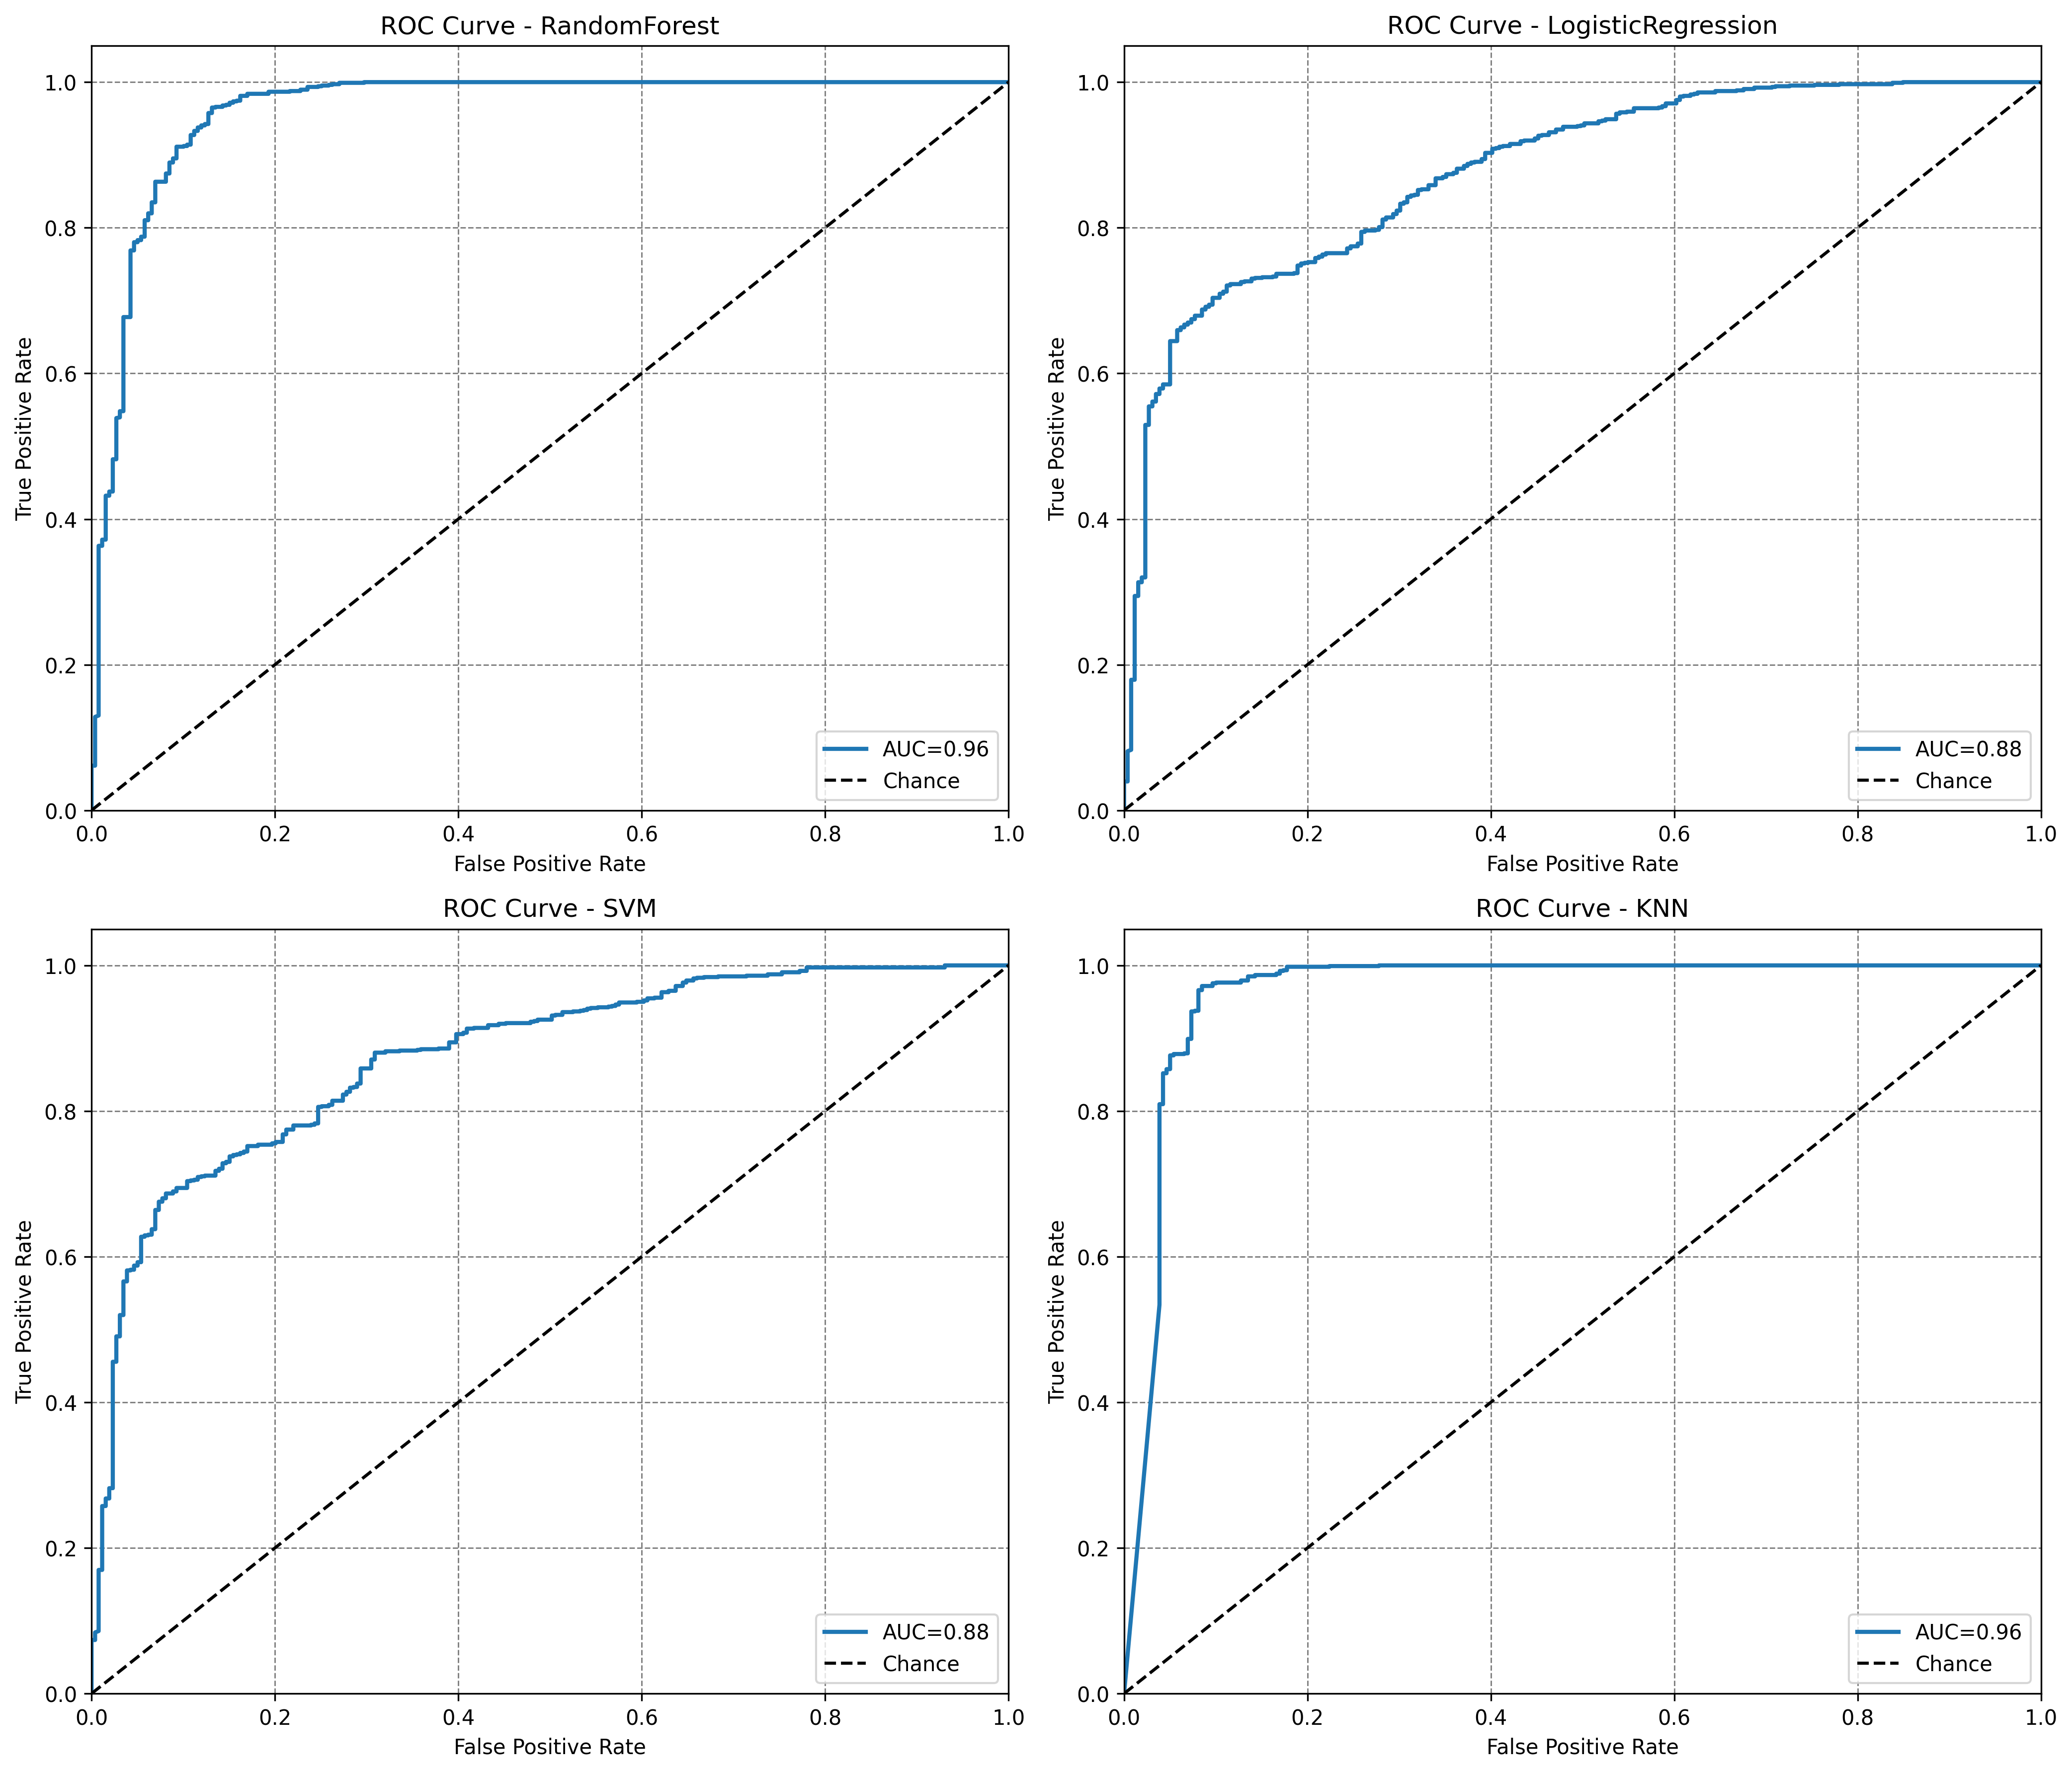
\includegraphics[width=\linewidth]{images/2x2_roc_curves_import_test_target.png}
		\caption{ROC Curve 2}
	\end{subfigure}
	\caption{ROC Curves for Protein Sequence-Based Embeddings}
	\label{fig:roc_sequence}
\end{figure}

\subsubsection{ROC Curves for Protein Protein Fold-Based Embeddings}
\begin{figure}[H]
	\centering
	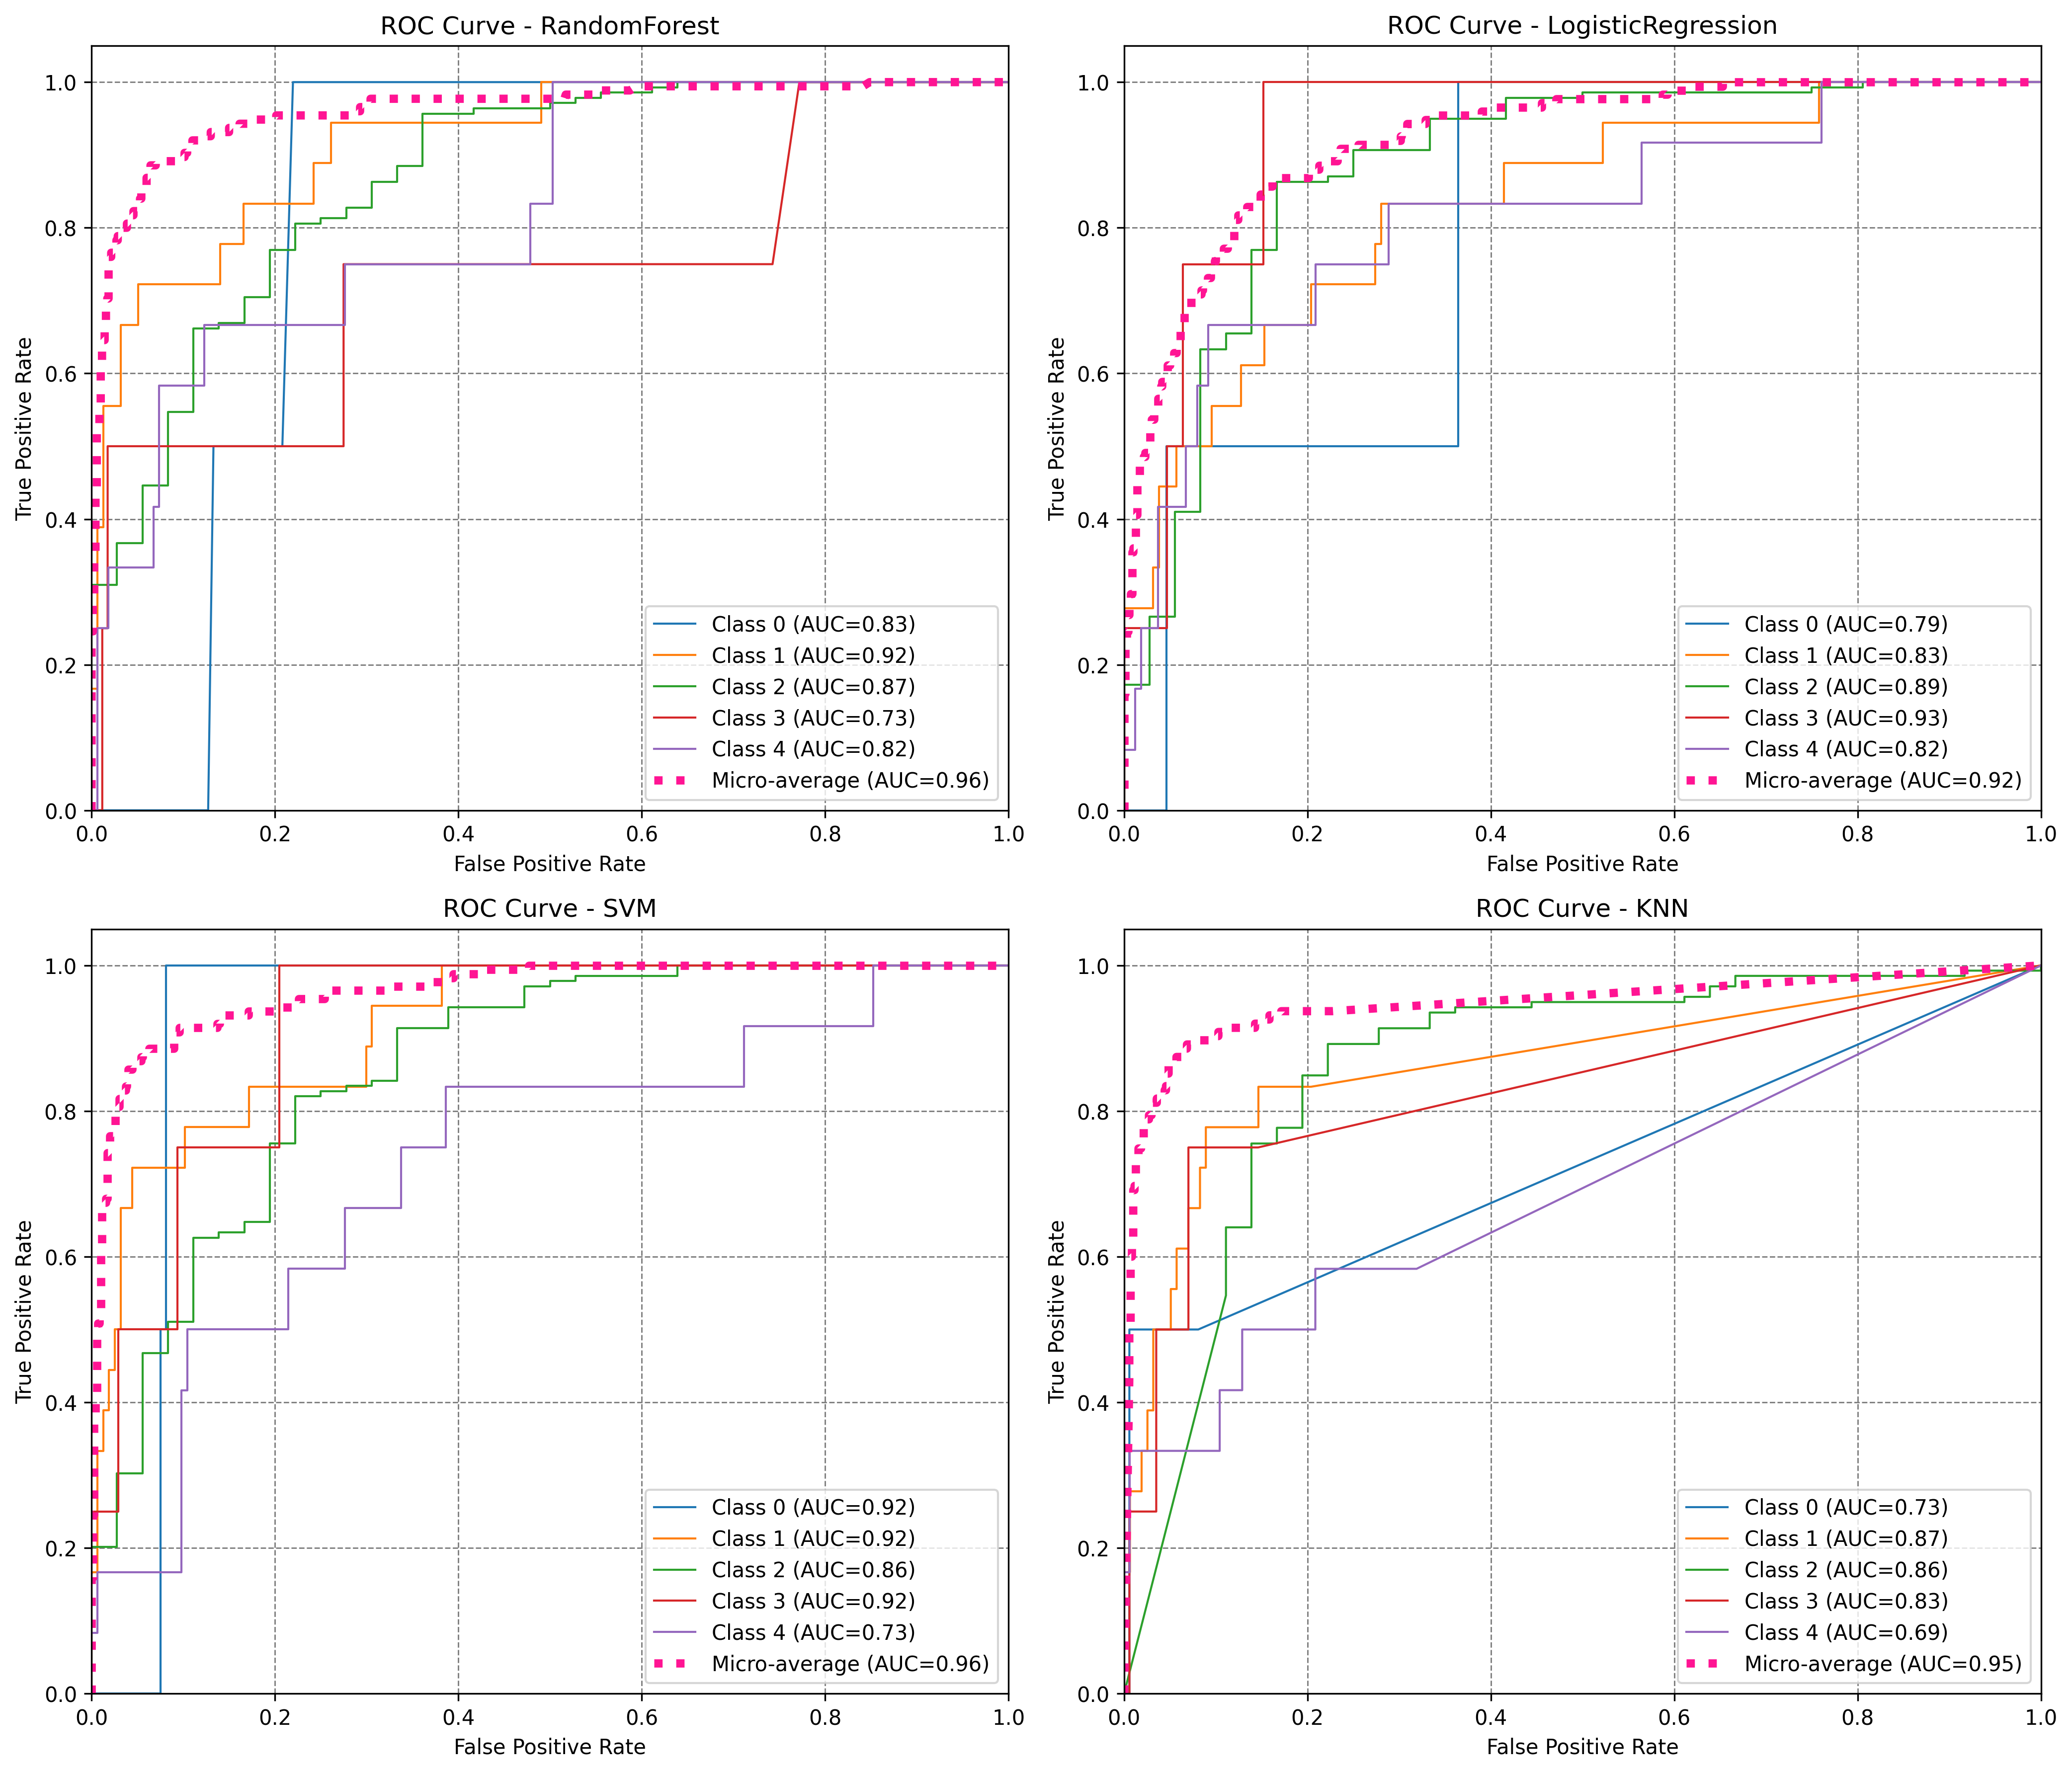
\includegraphics[width=0.7\textwidth]{images/2x2_roc_curves_folds_test_split.png}
	\caption{ROC Curve for Protein Fold-Based Embeddings}
	\label{fig:roc_fold}
\end{figure}

\subsubsection{Precision-Recall Curves for Protein Protein Sequence-Based Embeddings}
\begin{figure}[H]
	\centering
	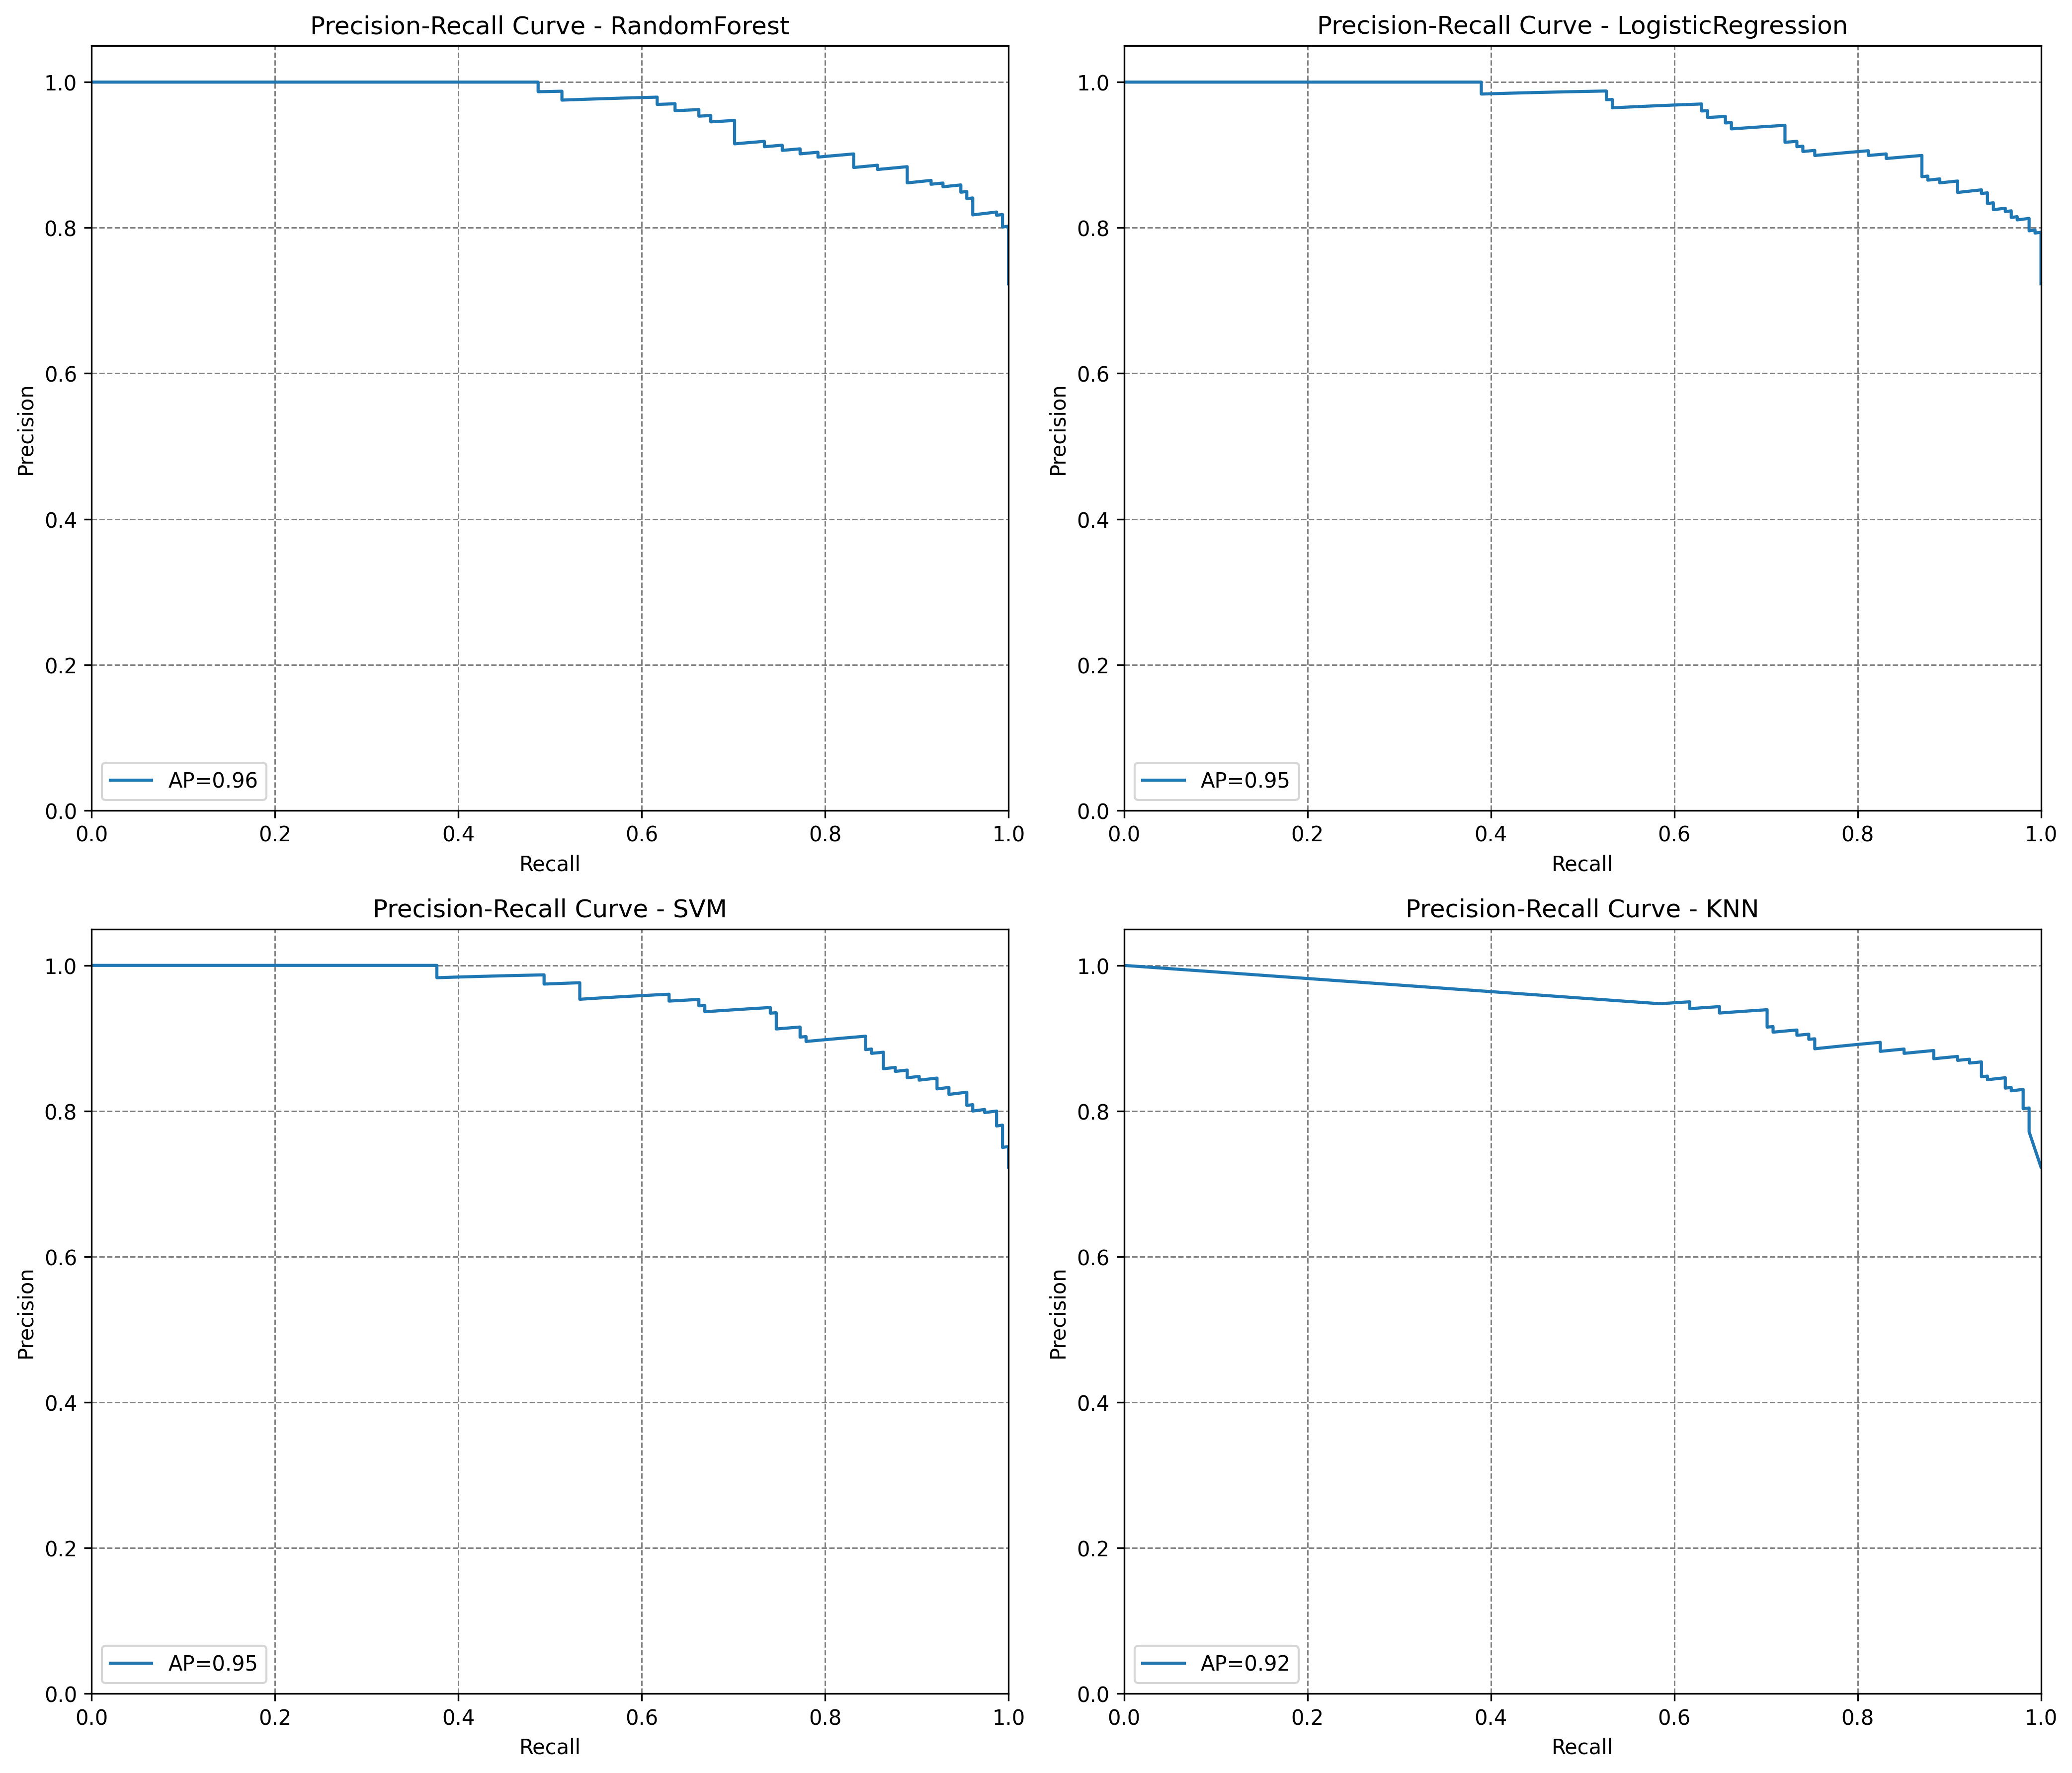
\includegraphics[width=0.7\textwidth]{images/2x2_precision_recall_curves_split_test_target.png}
	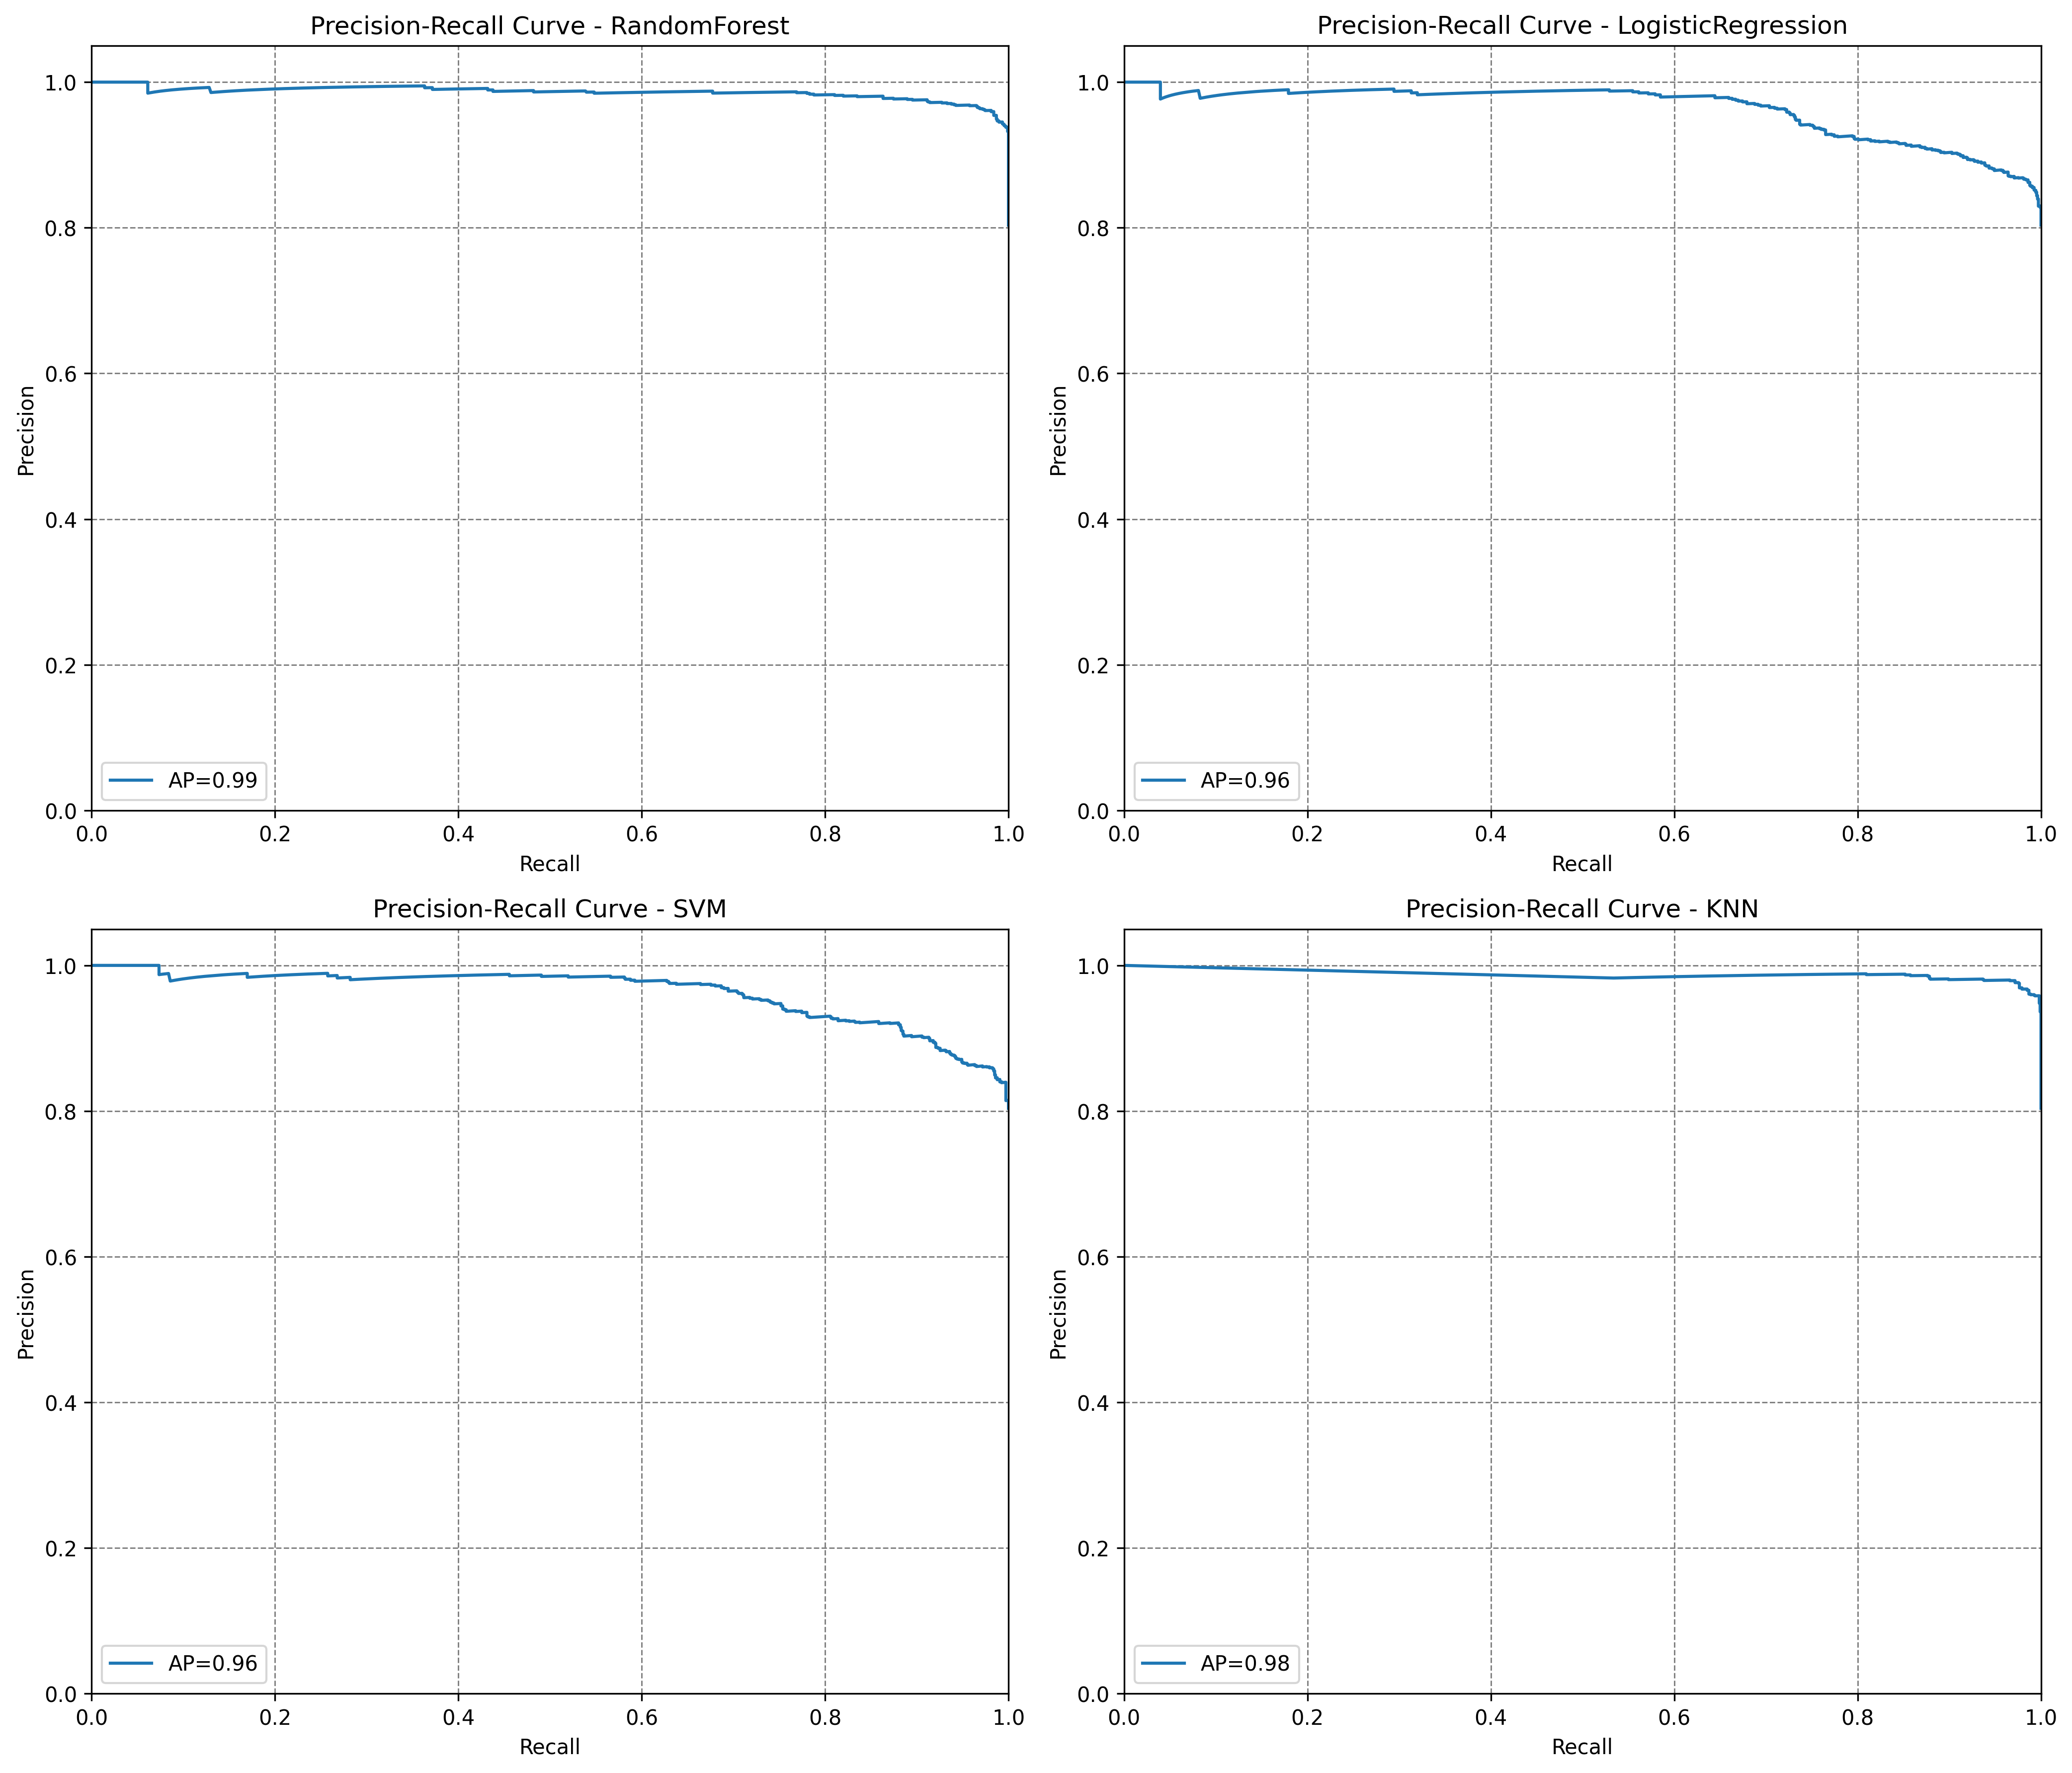
\includegraphics[width=0.7\textwidth]{images/2x2_precision_recall_curves_import_test_target.png}
	\caption{Precision-Recall Curves for Protein Sequence-Based Embeddings}
	\label{fig:pr_sequence}
\end{figure}

\subsubsection{Precision-Recall Curves for Protein Protein Fold-Based Embeddings}
\begin{figure}[H]
	\centering
	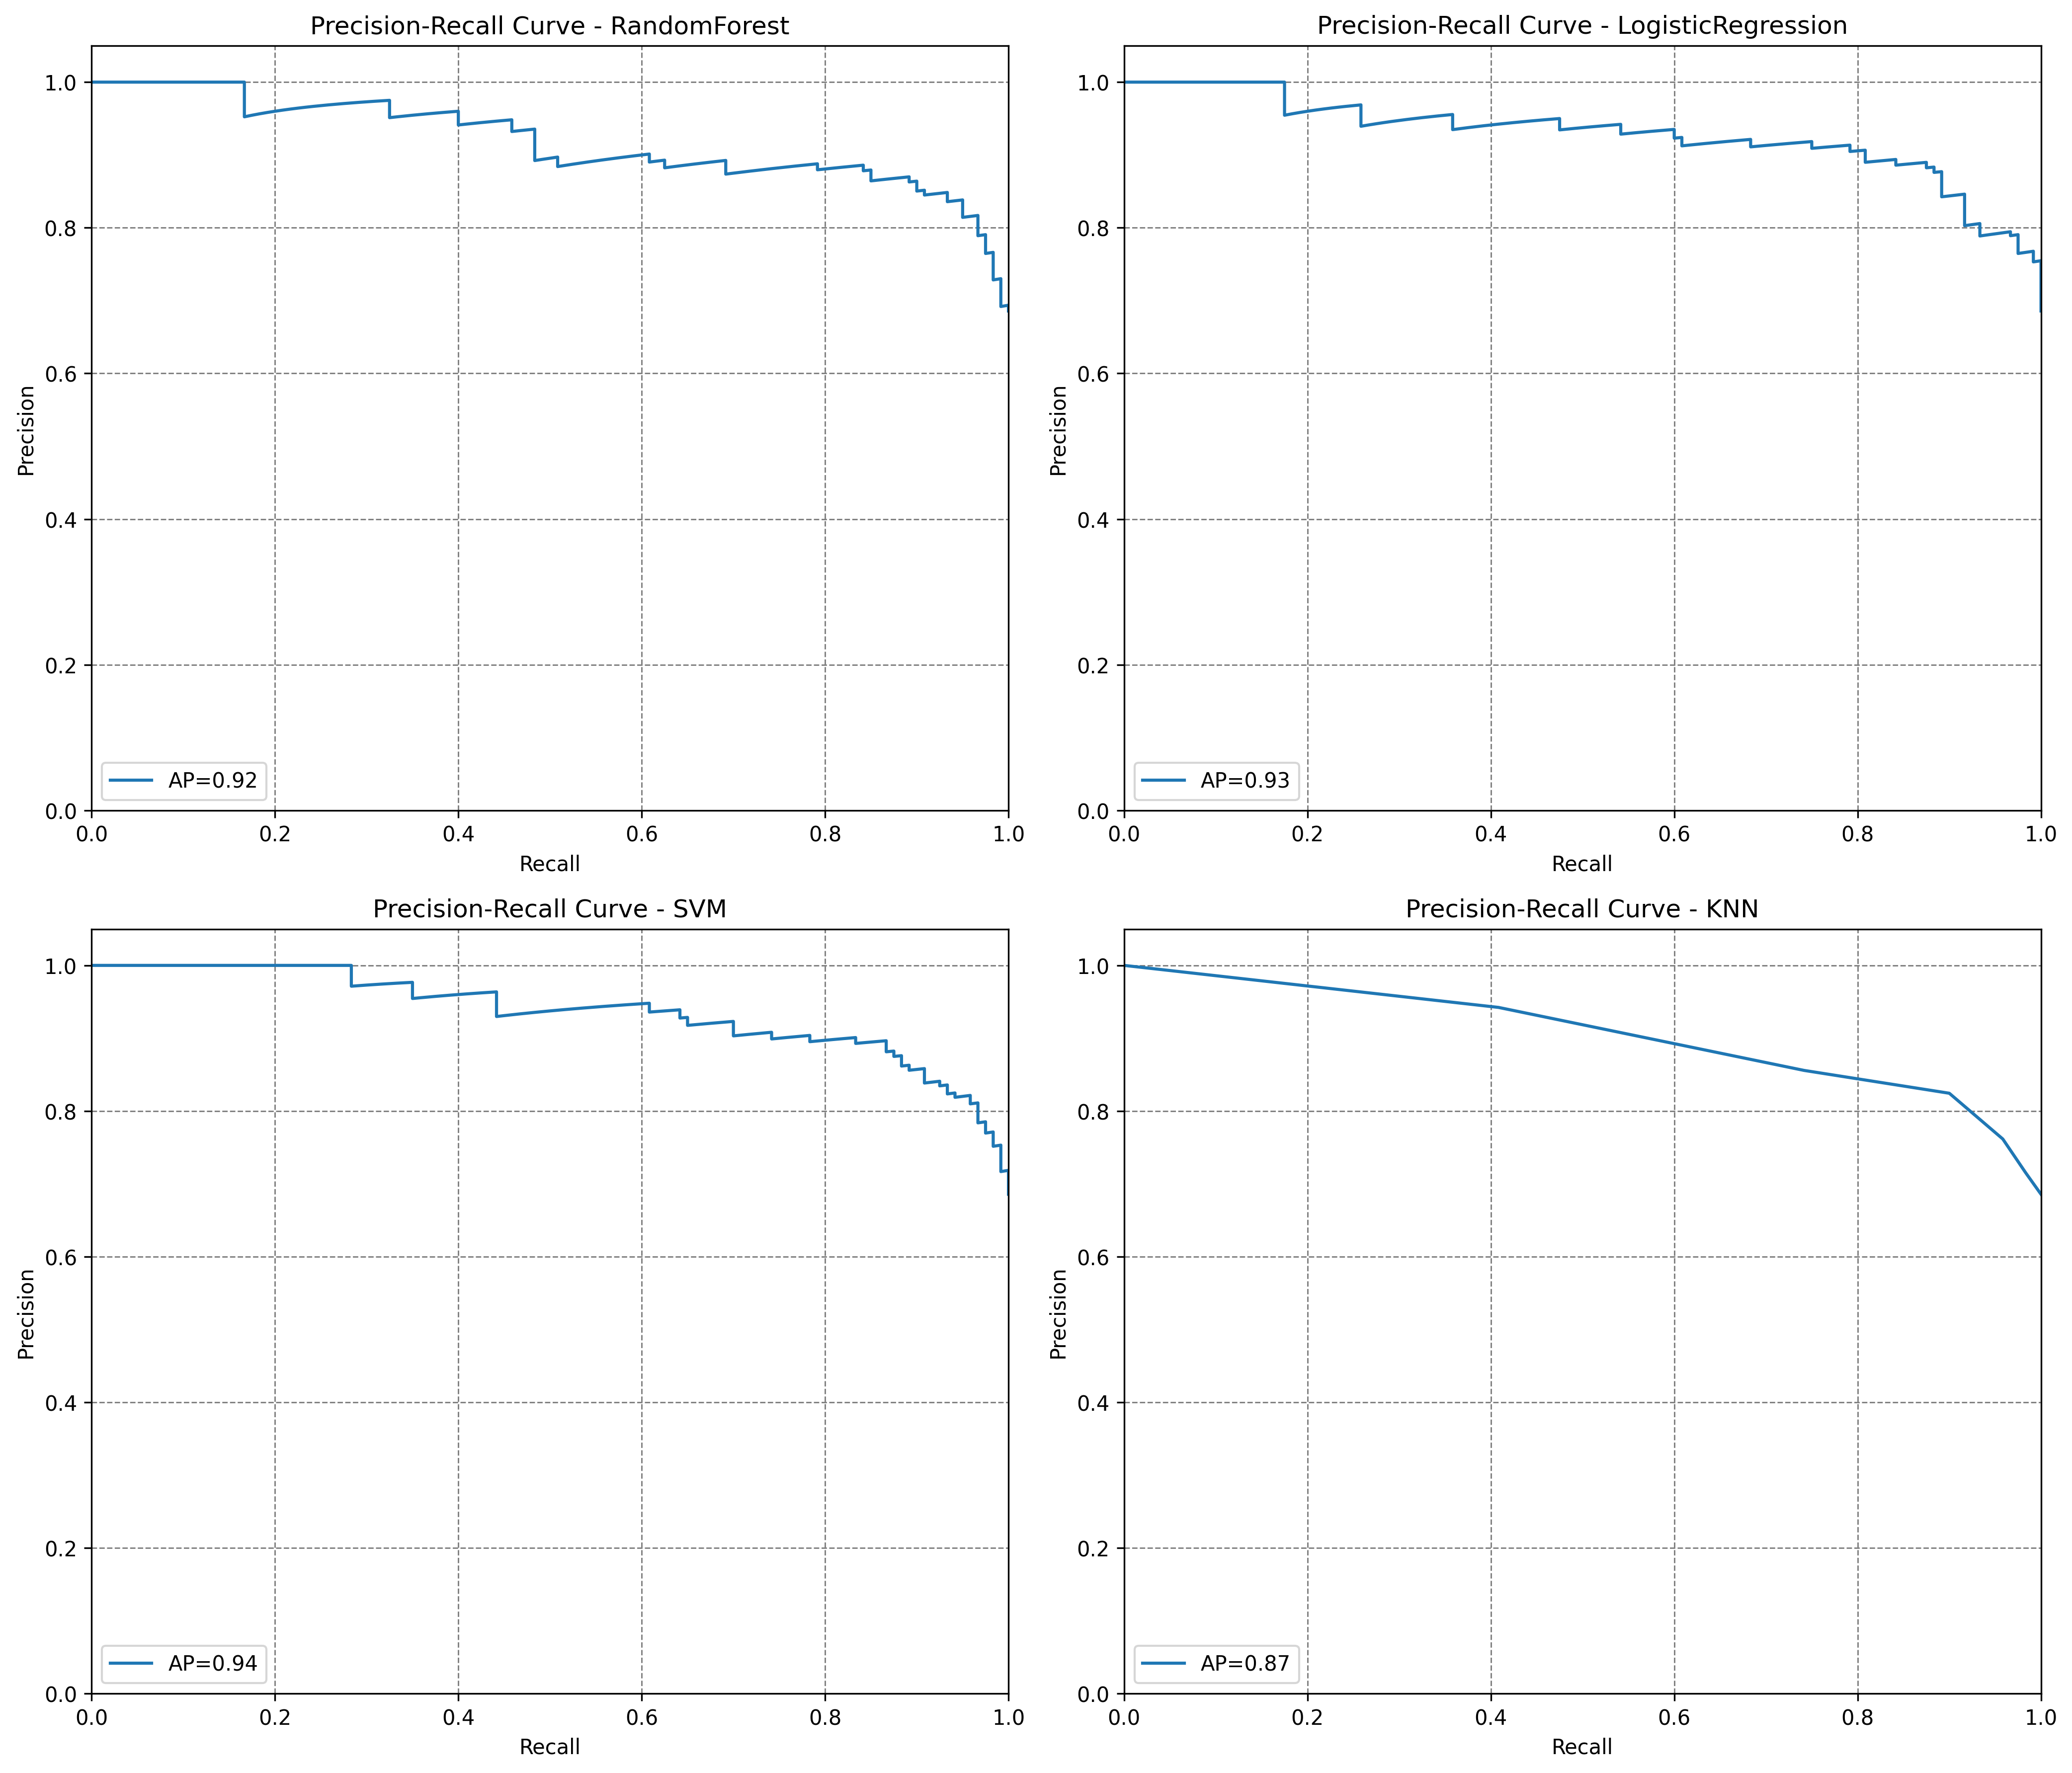
\includegraphics[width=0.8\textwidth,height=0.5\textwidth]{images/2x2_precision_recall_curves_target_folds_test_split.png}
	\caption{Precision-Recall Curve for Protein Fold-Based Embeddings}
	\label{fig:pr_fold}
\end{figure}

%\subsubsection{Confusion Matrices for Protein Protein Sequence-Based Embeddings}
%\begin{figure}[H]
%	\centering
%	\begin{subfigure}{0.49\textwidth}
%		\centering
%		\includegraphics[width=\linewidth]{images/conf_matrix_sequence1.jpg}
%		\caption{Confusion Matrix 1}
%	\end{subfigure}
%	\hfill
%	\begin{subfigure}{0.49\textwidth}
%		\centering
%		\includegraphics[width=\linewidth]{images/conf_matrix_sequence2.jpg}
%		\caption{Confusion Matrix 2}
%	\end{subfigure}
%	\caption{Confusion Matrices for Protein Sequence-Based Embeddings}
%	\label{fig:conf_matrix_sequence}
%\end{figure}

%\subsubsection{Confusion Matrices for Protein Protein Fold-Based Embeddings}
%\begin{figure}[H]
%	\centering
%	\includegraphics[width=0.7\textwidth]{images/conf_matrix_fold.jpg}
%	\caption{Confusion Matrix for Protein Fold-Based Embeddings}
%	\label{fig:conf_matrix_fold}
%\end{figure}


